% !TEX TS-program = arara
% arara: xelatex: { synctex: on, options: [--halt-on-error] } 
% arara: biber
% arara: makeglossaries
% arara: makeindex
% arara: xelatex: { synctex: on, options: [-halt-on-error]  } 
% arara: xelatex: { synctex: on, options: [-halt-on-error]   } 
% arara: clean: { files: [ interpolation-notes.aux] }
% arara: clean: { files: [ interpolation-notes.bcf, interpolation-notes.blg] }
% arara: clean: { files: [ interpolation-notes.glg, interpolation-notes.glo] }
% arara: clean: { files: [ interpolation-notes.gls, interpolation-notes.gls] }
% arara: clean: { files: [ interpolation-notes.idx, interpolation-notes.ilg] }
% arara: clean: { files: [ interpolation-notes.ind, interpolation-notes.loe] }
% arara: clean: { files: [ interpolation-notes.lof, interpolation-notes.log ] }
% arara: clean: { files: [ interpolation-notes.log, interpolation-notes.lol ] }
% arara: clean: { files: [ interpolation-notes.out ] }
% arara: clean: { files: [ interpolation-notes.run.xml] }
% arara: clean: { files: [ interpolation-notes.toc, interpolation-notes.xdy] }
% arara: clean: { files: [ interpolation-notes.synctex.gz] }
%-------------------------------------------------------------------------------
%\documentclass[10pt,openany]{book}
\documentclass[11pt,openany]{article}
% TODO:
% \usepackage{amsmath,amsfonts,amssymb,mathrsfs,theorem}
% \usepackage{multicol,multirow,calc,achicago,graphicx,color,colortab,rotating,enumerate}
% \usepackage{pstricks,psfrag,tabularx,comment,hyperref}
% \usepackage{boxedminipage}
% \usepackage{bbm}
% Graphics
% \usepackage{graphicx}
% %Tables
% \usepackage{booktabs}
% \usepackage{lscape}
% \usepackage{bbold}
% \usepackage{natbib}
% \def\newblock{\hskip .11em plus .33em minus .07em}
% \usepackage{url}
% \usepackage{citeref}
% \citestyle{authoryear}
% \usepackage{hyperref}

%-------------------------------------------------------------------------------
\errorcontextlines 10000
%-------------------------------------------------------------------------------
% layout file determines 1/2 col, landscape/portrait...
\usepackage{geometry}
%-------------------------------------------------------------------------------
\usepackage{color}
\usepackage[dvipsnames,svgnames,x11names]{xcolor}
%-------------------------------------------------------------------------------
\usepackage{graphics}
\usepackage{epsfig}
\usepackage{graphicx}
\PassOptionsToPackage{normalem}{ulem}
\usepackage{ulem}
%-------------------------------------------------------------------------------
\usepackage{url}
%-------------------------------------------------------------------------------
\usepackage[english]{babel}
%-------------------------------------------------------------------------------
%\usepackage{csquotes}
%-------------------------------------------------------------------------------
\usepackage{epigraph}
\setlength{\epigraphwidth}{\linewidth}
%-------------------------------------------------------------------------------
\usepackage{fontspec}
%-------------------------------------------------------------------------------
%\setmainfont{Baskerville Old Face}
%\setmainfont{Libre Caslon Text}[Scale=0.85]
%\setmainfont{Centaur}
%\setmainfont{Garamond}
%\setmainfont{Georgia}
%\setmainfont{Perpetua}
%\setmainfont{Poor Richard}

% http://www.impallari.com/projects/overview/libre-caslon-display-and-text
%\setmainfont{Libre Caslon Text}[Scale=0.85]
%\newfontfamily\scshape[Letters=SmallCaps,Scale=1.15]{Crimson}

% http://iginomarini.com/fell/the-revival-fonts/
% \fontspec[
%  SmallCapsFont=IM FELL English SC,
%  SmallCapsFeatures={Letters=SmallCaps},
% ]{IM FELL English}
% \setmainfont{IM FELL English}
 
% https://github.com/CatharsisFonts/Cormorant/releases/tag/v3.3 

% http://www.georgduffner.at/ebgaramond/download.html
% \fontspec[
%  SmallCapsFeatures={Letters=SmallCaps},
% ]{EB Garamond}
\setmainfont[
Path,
UprightFont = *12-Regular,
ItalicFont  = *12-Italic,
BoldFont    = *08-Regular,
BoldItalicFont = *08-Italic ]
{EBGaramond}

% https://www.microsoft.com/typography/fonts/family.aspx?FID=134
% \fontspec[
%  SmallCapsFeatures={Letters=SmallCaps},
% ]{Garamond}
% \setmainfont{Garamond}
%\setmainfont{Palatino Linotype}
%\setmainfont{Perpetua}[Scale=1.1]
%\setmainfont{Times New Roman}
%-------------------------------------------------------------------------------
% https://www.microsoft.com/typography/fonts/family.aspx?FID=155
\setsansfont{Gill Sans MT} 

% http://arkandis.tuxfamily.org/adffonts.html
% \setsansfont{Gillius ADF}
%-------------------------------------------------------------------------------
% \setmonofont{}
%-------------------------------------------------------------------------------
% \usepackage{xeCJK}
% \setCJKmainfont{SimHei}
% \setCJKsansfont{SimHei}
% \setCJKmonofont{Lucida Sans Typewriter}
%-------------------------------------------------------------------------------
\usepackage{amsmath}
\usepackage{amssymb}
\DeclareMathOperator*{\argmin}{argmin}
\DeclareMathOperator*{\argmax}{argmax}
\DeclareMathOperator*{\sign}{sign}
\DeclareMathOperator*{\defeq}
{\overset{\underset{\mathrm{def}}{}}{=}}
%\DeclareMathOperator*{\cdf}{cdf}
%\DeclareMathOperator*{\quantile}{quantile}
\newcommand\bigforall{\mbox{\Large $\mathsurround0pt\forall$}} 
%https://tex.stackexchange.com/questions/83509/hfill-in-math-mode
\makeatletter
\newcommand{\pushright}[1]{\ifmeasuring@#1\else\omit\hfill$\displaystyle#1$\fi\ignorespaces}
\newcommand{\pushleft}[1]{\ifmeasuring@#1\else\omit$\displaystyle#1$\hfill\fi\ignorespaces}
\newcommand{\specialcell}[1]{\ifmeasuring@#1\else\omit$\displaystyle#1$\ignorespaces\fi}\makeatother
\makeatother
% https://tex.stackexchange.com/questions/14071/how-can-i-increase-the-line-spacing-in-a-matrix
\makeatletter
\renewcommand*\env@matrix[1][\arraystretch]{%
  \edef\arraystretch{#1}%
  \hskip -\arraycolsep
  \let\@ifnextchar\new@ifnextchar
  \array{*\c@MaxMatrixCols c}}
\makeatother
% https://tex.stackexchange.com/questions/42726/align-but-show-one-equation-number-at-the-end/42728#42728
\newcommand\numberthis{\addtocounter{equation}{1}\tag{\theequation}}
%-------------------------------------------------------------------------------
\usepackage{mathtools}
%-------------------------------------------------------------------------------
\usepackage{amsthm}
%\theoremstyle{definition}
%\newtheorem{example}{Example}[section]
\usepackage{thmtools}
\theoremstyle{definition}
\DeclareRobustCommand{\rvspace}[1]{\vspace{#1}}
\declaretheoremstyle[
spaceabove=12pt,
spacebelow=10pt,
headpunct={\sffamily\mdseries:},
%headformat=margin,
headpunct={},
headfont=\sffamily\mdseries,
notefont=\sffamily\mdseries,
notebraces={}{},
bodyfont=\normalfont,
postheadspace=\newline,%
]{mythmstyle}
\declaretheorem[style=mythmstyle,title=Definition,name={Definition}]{definition}
\declaretheorem[style=mythmstyle,title=Example,name={Example}]{example}
\renewcommand{\thmtformatoptarg}[1]{#1}%
%\theoremstyle{definition}
%\newtheorem{definition}{\textsf{Definition}}[section]
%\newtheorem{fact}{\textsf{Fact}}[section]
%-------------------------------------------------------------------------------
\numberwithin{definition}{section}
\numberwithin{example}{section}
\numberwithin{equation}{section}
\numberwithin{figure}{section}
%-------------------------------------------------------------------------------
\usepackage{listings}
\lstset{backgroundcolor={\color{GhostWhite}},
basicstyle={\ttfamily\small},
breaklines=false,
captionpos=b,
%frame=tblr,
mathescape=true,
escapechar=\%,
keywordstyle={\ttfamily}}
\renewcommand{\lstlistingname}{Listing}
\providecommand{\algorithmname}{Algorithm}
\providecommand{\exercisename}{Exercise}
\providecommand{\theoremname}{Theorem}
\providecommand{\examplename}{Example}
%-------------------------------------------------------------------------------
% \makeatletter
% \let\orig@item\item
% 
% \def\item{%
%     \@ifnextchar{[}%
%         {\lstinline@item}%
%         {\orig@item}%
% }
% 
% \begingroup
% \catcode`\]=\active
% \gdef\lstinline@item[{%
%     \setbox0\hbox\bgroup
%         \catcode`\]=\active
%         \let]\lstinline@item@end
% }
% \endgroup
% 
% \def\lstinline@item@end{%
%     \egroup
%     \orig@item[\usebox0]%
% }
% \makeatother
%-------------------------------------------------------------------------------
\usepackage{algpseudocode,algorithm,algorithmicx}
%-------------------------------------------------------------------------------
\usepackage{datetime}
\renewcommand{\dateseparator}{-}
\renewcommand{\today}{
\the\year \dateseparator \twodigit\month \dateseparator \twodigit\day}
%-------------------------------------------------------------------------------
\setlength{\parskip}{5pt}
\setlength{\parindent}{0pt}
\usepackage[parfill]{parskip}
%-------------------------------------------------------------------------------
% \usepackage{fancyhdr}
% \pagestyle{fancy}
% \setlength{\headwidth}{\textheight}
% \addtolength{\headwidth}{\columnsep}
% %\addtolength{\headwidth}{\marginparsep}
% %\addtolength{\headwidth}{\marginparwidth}
% \fancypagestyle{plain}{
% \fancyhead{} % clear all head fields 
% \fancyfoot{} % clear all foot fields
% \fancyfoot[RO,LE]{\textsf{\thepage}} 
% \fancyfoot[RE,LO]{\textsf{Draft of \today}}
% \renewcommand{\headrulewidth}{0.0pt}
% \renewcommand{\footrulewidth}{0.1pt}}
% \pagestyle{plain}
%-------------------------------------------------------------------------------
\usepackage{titling}
%\newfontfamily\titlefont[Scale=MatchUppercase]{Gill Sans MT}
%\renewcommand{\maketitlehooka}{\titlefont}
\pretitle{\begin{flushright}\Huge\sffamily\bfseries}
\posttitle{\par\end{flushright}\vskip 0.25em}
\preauthor{\begin{flushright}\sffamily\scshape\mdseries}
\postauthor{\par\end{flushright}}
\predate{\begin{flushright}\sffamily\scshape\mdseries}
\postdate{\par\end{flushright}}
\setlength{\droptitle}{-80pt}
%-------------------------------------------------------------------------------
\usepackage{enumitem}
\setlist[description]{font=\small\sffamily\mdseries,style=unboxed,leftmargin=0cm}
\setlist[itemize]{style=unboxed,itemindent=0cm}
\setlist[enumerate]{style=unboxed,itemindent=0cm}
%-------------------------------------------------------------------------------
\usepackage[sf,small,compact]{titlesec}
%\newfontfamily\headingfont[]{New Yorker}
%\newfontfamily\headingfont[Scale=MatchUppercase]{Libre Caslon Display}
%\newfontfamily\headingfont[]{Perpetua Titling MT}
%\newfontfamily\headingfont[Scale=MatchUppercase]{Gill Sans MT}
%\newfontfamily\headingfont[Scale=MatchUppercase]{Gillius ADF}

\titleformat{\part}{\huge\sffamily\bfseries}{\thepart}{0.5em}{}
\titleformat{\chapter}{\LARGE\sffamily\bfseries}{\thechapter}{0.5em}{}
\titleformat{\section}{\Large\sffamily\bfseries}{\thesection}{0.5em}{}
\titleformat{\subsection}{\large\sffamily\bfseries}{\thesubsection}{0.5em}{}
\titleformat{\subsubsection}{\large\sffamily\mdseries}{\thesubsubsection}{0.5em}{}
\titleformat{\paragraph}[runin]{\normalsize\sffamily\mdseries}{\theparagraph}{0.5em}{}[\hspace{1em}]
\titleformat{\subparagraph}[runin]{\normalsize\sffamily\mdseries}{\thesubparagraph}{0.5em}{}[\hspace{1em}]

\titlespacing\section{0pt}{12pt plus 12pt minus 2pt}{5pt plus 5pt minus 2pt}
\titlespacing\subsection{0pt}{11pt plus 11pt minus 2pt}{5pt plus 5pt minus 2pt}
\titlespacing\subsubsection{0pt}{10pt plus 10pt minus 2pt}{5pt plus 5pt minus 2pt}

\setcounter{secnumdepth}{7}
%-------------------------------------------------------------------------------
\makeatletter
\let\oldl@chapter\l@chapter
\def\l@chapter#1#2{\oldl@chapter{#1}{\textsf{#2}}}
\let\old@dottedcontentsline\@dottedtocline
\def\@dottedtocline#1#2#3#4#5{%
\old@dottedcontentsline{#1}{#2}{#3}{#4}{{\textsf{#5}}}}
\makeatother
%-------------------------------------------------------------------------------
% \usepackage{tocloft}
% \renewcommand{\cftpartfont}{\sffamily}
% \renewcommand{\cftchapfont}{\sffamily}
% \renewcommand{\cftsecfont}{\sffamily}
% \renewcommand{\cftsubsecfont}{\sffamily}
% \renewcommand{\cftsubsubsecfont}{\sffamily}
% \renewcommand{\cftparafont}{\sffamily}
% \renewcommand{\cftsubparafont}{\sffamily}
%-------------------------------------------------------------------------------
\usepackage{enumitem}
%\setlist[description]{font=\small\sffamily\mdseries,style=unboxed,leftmargin=0cm}
\setlist[description]{font=\sffamily\mdseries}
% \setlist[itemize]{style=unboxed,itemindent=0cm}
% \setlist[enumerate]{style=unboxed,itemindent=0cm}
%-------------------------------------------------------------------------------
%https://en.wikibooks.org/wiki/LaTeX/Indexing
\usepackage{makeidx}
\makeindex
\usepackage[totoc]{idxlayout}
%-------------------------------------------------------------------------------
\usepackage[
backend=biber, 
citestyle=numeric-comp, 
bibstyle=numeric,
%bibstyle=verbose,
%entrykey=false,
labelnumber=true,
sortcites=true,
maxnames=1000,
maxitems=1000,
block=nbpar,
abbreviate=false,
date=edtf,
alldates=edtf,
datezeros=true,
timezeros=true,
]{biblatex} 
\renewcommand\mkbibnamefamily[1]{\textsc{#1}}
%-------------------------------------------------------------------------------
% \usepackage[chapter]{tocbibind}
% \renewcommand{\listfigurename}{Figures}
% \setlofname{Figures}
% \renewcommand{\listoffigures}{\begingroup
% \tocchapter
% \tocfile{\listfigurename}{lof}
% \endgroup}
%-------------------------------------------------------------------------------
%\usepackage[titletoc]{appendix}
%-------------------------------------------------------------------------------
\usepackage[unicode=true,pdfusetitle,
 bookmarks=true,bookmarksnumbered=false,bookmarksopen=true,bookmarksopenlevel=1,
 breaklinks=false,pdfborder={0 0 0},backref=false,colorlinks=true]{hyperref}
% these renewcommands don't seem to work
% \renewcommand{\chapterautorefname}{\S}
% \renewcommand{\sectionautorefname}{\S}
% \renewcommand{\subsectionautorefname}{\S}
% \renewcommand{\subsubsectionautorefname}{\S}
\hypersetup{unicode=true,
colorlinks=true,
pdfpagemode=UseOutlines,
pdfpagelayout=OneColumn,
pdfstartview=Fit,
linkcolor=MidnightBlue,
urlcolor=Mahogany,
citecolor=OliveGreen}
%-------------------------------------------------------------------------------
% %\usepackage[xindy,toc,style=alttreehypergroup,nolong,nosuper]{glossaries}
% \usepackage[xindy,toc,style=alttreehypergroup,nolong,nosuper]{glossaries}
%-------------------------------------------------------------------------------

%jam 2004-09-10

\def\Boundary{\partial}
\def\Vvertex{\nu}
\def\Ssimplex{\sigma}
\def\Tsimplex{\tau}
\def\Rsimplex{\rho}
\def\Ffacet{\phi}
\def\Eedge{\epsilon}
\def\Kcomplex{\mathcal{K}}  % An abstract simplicial complex
\def\Mmesh{\mathcal{M}}  % A simplicial mesh

\def\Set#1{{\mathcal{#1}}} 
\def\Space#1{{\mathbb{#1}}} 
\def\Vector#1{{\mathsf{#1}}} 

\def\Sset{\mathcal{S}}    % generic set

\def\Integers{\mathbb{Z}}
\def\Reals{\mathbb{R}}    % Real numbers
\def\Quaternions{\mathbb{Q}}    % set of Quaternions

\def\Uspace{\mathbb{U}}  % vector space
\def\Vspace{\mathbb{V}}  % vector space
\def\Wspace{\mathbb{W}}  % vector space

\def\Aspace{\mathbb{A}}  % affine space
\def\Tspace{\mathbb{T}}  % translation space (of an affine space)

\def\Lspace{\mathbb{L}} % space of of linear maps

\def\t{\mathsf{t}} % translation vector
\def\u{\mathsf{u}} % vector
\def\v{\mathsf{v}} % vector
\def\w{\mathsf{w}} % vector
\def\0{{\mathsf 0}} % zero vector
\def\e{\mathsf{e}} % canonical basis vector
\def\b{\mathsf{b}} % barycentric coord. $\b_i$, $\b_{i,j}$

\def\p{\mathsf{p}}     % generic point
\def\q{\mathsf{q}}     % generic point
\def\r{\mathsf{r}}     % generic point

\def\f{\mathsf{f}}     % generic vector-valued function
\def\g{\mathsf{g}}     % generic vector-valued function
\def\h{\mathsf{h}}     % generic vector-valued function

\def\Umap{\mathsf{U}}  % matrix whose cols are ui
\def\Vmap{\mathsf{V}}  % matrix whose cols are vi
\def\Wmap{\mathsf{W}}  % matrix whose cols are wi

\def\Lmap{\mathsf{L}} % linear transform
\def\Mmap{\mathsf{M}} % another linear transform

\def\Emap{\mathsf{E}} % canonical basis vector for space of linear transforms
\def\Tmap{\mathsf{T}}  % translation
\def\Amap{\mathsf{A}} % affine transform

\def\c{\mathsf{c}} % row of \Lmap linear transform
\def\r{\mathsf{r}} % row of \Lmap linear transform

\def\Identity{\mathsf{I}}   % the identity transformation

\def\union{\cup}
\def\intersection{\cap}
\def\Union{\bigcup}
\def\Intersection{\bigcap}

\def\Transpose{\mathrm{transpose}}   % the transpose transformation
\def\LTL{\mathrm{LTL}}   % a-transpose-a
\def\Inverse{\mathrm{inverse}}
\def\Pseudoinverse{\mathrm{pseudoinverse}}

\def\dimension{\mathrm{dim}}   % dimension of geometric object
\def\Projection{\pi}   % orthogonal projection

\def\kernel{\mathrm{ker}}    % kernel
\def\range{\mathrm{ran}}    % range
\def\linearspan{\mathrm{span}}    % linear span
\def\affinespan{\mathrm{aff}}    % affine span
\def\convexspan{\mathrm{hull}}    % convex span, convex hull

\def\volume{\mathrm{volume}}    % sign function

\def\Da#1{{\mathcal{D}{#1}}}    % derivative operator
\def\Db#1#2{{\mathcal{D}{#1}_{\mid_{#2}}}}    % derivative operator
\def\Dc#1#2#3{{\mathcal{D}{#1}_{\mid_{#2}}({#3})}}  % derivative operator
\def\Dd#1#2#3#4{{\mathcal{D}_{#1}{{#2}}_{\mid_{#3}}({{#4}})}} % derivative operator
\def\De#1#2#3{{\mathcal D}_{#1}{#2}_{\mid_{#3}}}  % derivative operator
\def\Df#1#2{{\mathcal D}_{#1}{#2}}  % derivative operator

\def\da#1#2{{\partial}_{#1}{#2}}  % partial derivative operator
\def\db#1#2#3{{\partial}_{#1}{#2}_{\mid_{#3}}}  % partial derivative operator

\def\Ga#1{{\mathbf \nabla}{#1}}   % derivative operator
\def\Gb#1#2{{\mathbf \nabla}{#1}_{\mid_{#2}}} % derivative operator
\def\Gc#1#2#3{{\mathbf \nabla}_{#1}{{#2}}_{\mid_{#3}}}  % derivative operator
\def\Gf#1#2{{\mathbf \nabla}_{#1}{#2}}  % derivative operator

\def\Edges{\mathcal{E}}                   % edges
\def\Faces{\mathcal{F}}                   % faces

\def\Q{\mathsf{Q}} % Transform corresponding to quaternion
\def\R{\mathsf{R}} % Rotation
\def\G{\mathsf{G}} % riGid transform
\def\Sc{\mathsf{S}}    % scaled rotation or subdivision transform

\def\sign{\mathrm{sign}}    % sign function

\def\dn{{\mathsf \delta \n}} % change in normal
\def\nd{{\mathsf \n^\bullet}} % dot product of adjacent normals

\def\a{\mathsf{a}}     % area-weighted face normal
\def\l{\mathsf{l}}     % Linear map as vector
\def\n{\mathsf{n}}     % unit length face normal
\def\x{\mathsf{x}}     % instance of point $\x$, $\x_i \in X$
\def\c{\mathsf{c}}     % 3d cross product as function
\def\d{\mathsf{d}}     % data record
\def\y{\mathsf{y}}     % another barycentric coordinate
\def\z{\mathsf{z}}     % projection of a point
\def\S{\mathsf{S}}     % local subdivision matrix


%\geometry{
%showframe=true,
%showcrop=true,
twoside=false,
twocolumn=false,
landscape=false,
margin=2mm,
%columnsep=12mm,
paperheight=160mm,
paperwidth=120mm}
%-------------------------------------------------------------------------------
\usepackage{fancyhdr}
\pagestyle{fancy}
%\setlength{\headwidth}{2 \columnwidth}
%\addtolength{\headwidth}{\columnsep}
\setlength{\headwidth}{\textwidth}
\fancypagestyle{plain}{
\fancyhead{} % clear all head fields 
\fancyfoot{} % clear all foot fields
\fancyfoot[R]{\textsf{\thepage}} 
\fancyfoot[L]{\textsf{Draft of \today}}
\renewcommand{\headrulewidth}{0.0pt}
\renewcommand{\footrulewidth}{0.1pt}}
\pagestyle{plain}

\geometry{
twoside=false,
twocolumn=true,
margin=2cm,
columnsep=2.5cm,
paperheight=340mm,
paperwidth=160mm,
landscape}

%input{../landscape-2col-9x16}
%\geometry{
twoside=false,
twocolumn=true,
margin=2cm,
columnsep=2.5cm,
paperheight=297mm,
paperwidth=210mm,
landscape}

%\geometry{
twoside=false,
twocolumn=true,
margin=2cm,
columnsep=2.5cm,
paperheight=279mm,
paperwidth=216mm,
landscape}

%\geometry{
twoside=false,
twocolumn=true,
margin=2cm,
columnsep=2.5cm,
paperheight=356mm,
paperwidth=216mm,
landscape}

%\usepackage{geometry}
\geometry{twoside,margin=2cm,
columnsep=2cm,
paperheight=297mm,paperwidth=210mm}

\lstdefinelanguage{clojure}%
{morekeywords={
%Math,Random,List,ArrayList,
deftest,testing,is,defrecord,
*,*1,*2,*3,*agent*,*allow-unresolved-vars*,*assert*,*clojure-version*,*command-line-args*,%
*compile-files*,*compile-path*,*e,*err*,*file*,*flush-on-newline*,*in*,*macro-meta*,%
*math-context*,*ns*,*out*,*print-dup*,*print-length*,*print-level*,*print-meta*,*print-readably*,%
*read-eval*,*source-path*,*use-context-classloader*,*warn-on-reflection*,+,-,->,->>,..,
%/,
:else,%
<,<=,=,==,>,>=,@,accessor,aclone,add-classpath,add-watch,agent,agent-errors,aget,alength,alias,%
all-ns,alter,alter-meta!,alter-var-root,amap,ancestors,and,apply,areduce,array-map,aset,%
aset-boolean,aset-byte,aset-char,aset-double,aset-float,aset-int,aset-long,aset-short,assert,%
assoc,assoc!,assoc-in,associative?,atom,await,await-for,await1,bases,bean,bigdec,bigint,binding,%
bit-and,bit-and-not,bit-clear,bit-flip,bit-not,bit-or,bit-set,bit-shift-left,bit-shift-right,%
bit-test,bit-xor,boolean,boolean-array,booleans,bound-fn,bound-fn*,butlast,byte,byte-array,%
bytes,cast,char,char-array,char-escape-string,char-name-string,char?,chars,chunk,chunk-append,%
chunk-buffer,chunk-cons,chunk-first,chunk-next,chunk-rest,chunked-seq?,class,class?,%
clear-agent-errors,clojure-version,coll?,comment,commute,comp,comparator,compare,compare-and-set!,%
compile,complement,concat,cond,condp,conj,conj!,cons,constantly,construct-proxy,contains?,count,%
counted?,create-ns,create-struct,cycle,dec,decimal?,declare,def,definline,defmacro,defmethod,%
defmulti,defn,defn-,defonce,defprotocol,defstruct,deftype,delay,delay?,deliver,deref,derive,%
descendants,destructure,disj,disj!,dissoc,dissoc!,distinct,distinct?,do,do-template,doall,doc,%
dorun,doseq,dosync,dotimes,doto,double,double-array,doubles,drop,drop-last,drop-while,empty,empty?,%
ensure,enumeration-seq,eval,even?,every?,false,false?,ffirst,file-seq,filter,finally,find,find-doc,%
find-ns,find-var,first,float,float-array,float?,floats,flush,fn,fn?,fnext,for,force,format,future,%
future-call,future-cancel,future-cancelled?,future-done?,future?,gen-class,gen-interface,gensym,%
get,get-in,get-method,get-proxy-class,get-thread-bindings,get-validator,hash,hash-map,hash-set,%
identical?,identity,if,if-let,if-not,ifn?,import,in-ns,inc,init-proxy,instance?,int,int-array,%
integer?,interleave,intern,interpose,into,into-array,ints,io!,isa?,iterate,iterator-seq,juxt,%
key,keys,keyword,keyword?,last,lazy-cat,lazy-seq,let,letfn,line-seq,list,list*,list?,load,load-file,%
load-reader,load-string,loaded-libs,locking,long,long-array,longs,loop,macroexpand,macroexpand-1,%
make-array,make-hierarchy,map,map?,mapcat,max,max-key,memfn,memoize,merge,merge-with,meta,%
method-sig,methods,min,min-key,mod,monitor-enter,monitor-exit,name,namespace,neg?,new,newline,%
next,nfirst,nil,nil?,nnext,not,not-any?,not-empty,not-every?,not=,ns,ns-aliases,ns-imports,%
ns-interns,ns-map,ns-name,ns-publics,ns-refers,ns-resolve,ns-unalias,ns-unmap,nth,nthnext,num,%
number?,odd?,or,parents,partial,partition,pcalls,peek,persistent!,pmap,pop,pop!,pop-thread-bindings,%
pos?,pr,pr-str,prefer-method,prefers,primitives-classnames,print,print-ctor,print-doc,print-dup,%
print-method,print-namespace-doc,print-simple,print-special-doc,print-str,printf,println,println-str,%
prn,prn-str,promise,proxy,proxy-call-with-super,proxy-mappings,proxy-name,proxy-super,%
push-thread-bindings,pvalues,quot,rand,rand-int,range,ratio?,rational?,rationalize,re-find,%
re-groups,re-matcher,re-matches,re-pattern,re-seq,read,read-line,read-string,recur,reduce,ref,%
ref-history-count,ref-max-history,ref-min-history,ref-set,refer,refer-clojure,reify,%
release-pending-sends,rem,remove,remove-method,remove-ns,remove-watch,repeat,repeatedly,%
replace,replicate,require,reset!,reset-meta!,resolve,rest,resultset-seq,reverse,reversible?,%
rseq,rsubseq,second,select-keys,send,send-off,seq,seq?,seque,sequence,sequential?,set,set!,%
set-validator!,set?,short,short-array,shorts,shutdown-agents,slurp,some,sort,sort-by,sorted-map,%
sorted-map-by,sorted-set,sorted-set-by,sorted?,special-form-anchor,special-symbol?,split-at,%
split-with,str,stream?,string?,struct,struct-map,subs,subseq,subvec,supers,swap!,symbol,symbol?,%
sync,syntax-symbol-anchor,take,take-last,take-nth,take-while,test,the-ns,throw,time,to-array,%
to-array-2d,trampoline,transient,tree-seq,true,true?,try,type,unchecked-add,unchecked-dec,%
unchecked-divide,unchecked-inc,unchecked-multiply,unchecked-negate,unchecked-remainder,%
unchecked-subtract,underive,unquote,unquote-splicing,update-in,update-proxy,use,val,vals,%
var,var-get,var-set,var?,vary-meta,vec,vector,vector?,when,when-first,when-let,when-not,%
while,with-bindings,with-bindings*,with-in-str,with-loading-context,with-local-vars,%
with-meta,with-open,with-out-str,with-precision,xml-seq,zero?,zipmap
},%
   sensitive,% ???
   alsodigit=-,%
   morecomment=[l];,%
   morestring=[b]"%
  }[keywords,comments,strings]%

%-------------------------------------------------------------------------------
\newcommand{\aSet}[1]{\ensuremath{\mathcal{#1}}}
\newcommand{\aSpace}[1]{\ensuremath{\mathbb{#1}}}
\newcommand{\aVector}[1]{\ensuremath{\vec{#1}}}
\newcommand{\aPoint}[1]{\ensuremath{\mathbf{#1}}}
\newcommand{\setSpec}[2]{\ensuremath{\{#1 | #2\}}}
%-------------------------------------------------------------------------------
%\usepackage[xindy,toc,style=alttreehypergroup,nolong,nosuper]{glossaries}
\usepackage[xindy,toc,style=alttreehypergroup,nolong,nosuper]{glossaries}
%-------------------------------------------------------------------------------
% The alttree type of glossary styles need to know the
 % widest entry name for each level
\glssetwidest{Rational numbers} % level 0 widest name
\glssetwidest[1]{Homogeneous space}      % level 1 widest name
\makeglossaries

\newglossarystyle{cites}
{% based on list style
  \setglossarystyle{list}%
    \renewcommand*{\glossentry}[2]{%
    \item[\glsentryitem{##1}%
          \glstarget{##1}{\glossentryname{##1}}]
       \glossentrydesc{##1}\glspostdescription
    \ifglshasfield{useri}{##1}{\space
     % in the event of multiple cites (as in the vestibulum2
     % sample entry), \glsentryuseri{##1} needs to be expanded
     % before being passed to \cite.
     \glsletentryfield{\thiscite}{##1}{useri}%
     (See \expandafter\cite\expandafter{\thiscite})}{}%
    \space ##2}%
}

\newglossarystyle{citeshyper}
{% based on list style
  \setglossarystyle{alttreehypergroup}%
    \renewcommand*{\glossentry}[2]{%
    \item[\glsentryitem{##1}%
          \glstarget{##1}{\glossentryname{##1}}]
       \glossentrydesc{##1}\glspostdescription
    \ifglshasfield{useri}{##1}{\space
     % in the event of multiple cites (as in the vestibulum2
     % sample entry), \glsentryuseri{##1} needs to be expanded
     % before being passed to \cite.
     \glsletentryfield{\thiscite}{##1}{useri}%
     (See \expandafter\cite\expandafter{\thiscite})}{}%
    \space ##2}%
}
%-----------------------------------------------------------------
\newglossaryentry{Sets}{
  name={Sets},
  text={Sets},
  description={\nopostdesc},
  user1=Halmos1960Naive}

\newglossaryentry{Spaces}{
  name={Spaces},
  text={Spaces},
  description={\nopostdesc}}

  
\newglossaryentry{Set}{
  name={Set},
  text={set},
  first={a generic set},
  symbol={\aSet{S}},
  description={a generic \emph{set}},
  sort=set,
  parent=Sets}
  
\newglossaryentry{HomogeneousSpace}{
  name={Homogeneous Space},
  text={Homogeneous space},
  %first={a generic set},
  %symbol={\ensuremath{\mathcal{S}}},
  description={a \emph{space} where every point looks the same},
  %sort=set,
  parent=Spaces}
  
\newglossaryentry{elementOf}{
  name={elementOf},
  text={elementOf},
  first={elementOf},
  description={$x \in \mathcal{S}$ means $x$ is an element of
  the set $\mathcal{S}$}, 
  sort=element,
  symbol={\ensuremath{\in}},
  parent=Sets}

\newglossaryentry{Integers}{
  name={integers},
  text={integers},
  symbol={\aSpace{Z}},
  description={the integers}}

\newglossaryentry{PositiveIntegers}{
  name={positive integers},
  text={positive integers},
  symbol={\ensuremath{\aSpace{Z}_{+}}},
  description={\setSpec{i\glssymbol{elementOf}\glssymbol{Integers}}{i>0}},
  parent=Integers}

\newglossaryentry{NaturalNumbers}{
  name={natural numbers},
  text={natural numbers},
  symbol={\aSpace{N}},
  description={\setSpec{i\glssymbol{elementOf}\glssymbol{Integers}}{i \geq 0}}}

\newglossaryentry{RationalNumbers}{
  name={rational numbers},
  text={rational numbers},
  symbol={\aSpace{Q}},
  description={
  \setSpec{i/j}{
  i \glssymbol{elementOf} \glssymbol{Integers}, 
  j \glssymbol{elementOf} \glssymbol{PositiveIntegers}}}}

\newglossaryentry{RealNumbers}{
  name={real numbers},
  text={real numbers},
  symbol={\aSpace{R}},
  description={the real numbers}}

\newglossaryentry{DoublePrecisionFloat}{
  name={doubles},
  text={doubles},
  symbol={\aSpace{D}},
  description={the IEEE 754 64 bit floating point numbers}}

\newglossaryentry{SinglePrecisionFloat}{
  name={floats},
  text={floats},
  symbol={\aSpace{F}},
  description={the IEEE 754 32 bit floating point numbers}}

\newglossaryentry{GenericSpace}{
  name={a generic space},
  text={a generic space},
  symbol={\aSpace{S}},
  description={a generic space}}


%-----------------------------------------------------------------
% \def\M{{\mathcal M}}                   % A mesh
% \def\V{{\mathcal V}}                   % vertices 
% \def\E{{\mathcal E}}                   % edges
% \def\F{{\mathcal F}}                   % faces
% \def\Ta{{\mathcal T}} % registration target
% \def\I{{\mathbf I}}		% the identity transformation
% \def\Tr{{\mathbf T}} % registration transform
% \def\Eu{{\mathbf E}} % Euclidean transform
% \def\Q{{\mathbf Q}} % Transform corresponding to quaternion
% \def\R{{\mathbf R}} % Rotation
% \def\G{{\mathbf G}} % riGid transform
% \def\A{{\mathbf A}} % affine transform
% \def\L{{\mathbf L}} % linear transform
% \def\Sc{{\mathbf S}}    % scaled rotation or subdivision transform
% \def\t{{\mathbf t}} % translation vector
% \def\v{{\mathbf v}}                   % vertex 
% \def\e{{\mathbf e}}                   % edge
% \def\f{{\mathbf f}}                   % face
% \def\s{{\mathbf s}}                   % simplex
% \def\w{{\mathbf w}}                   % vector of unconstrained weights
% \def\P{{\mathbf P}}                   % vector of unconstrained weights
% \def\u{{\mathbf u}}                   % vector of convex weights
% 
% \def\etal{{\it et al.}}
% 
% \def\Re{\mathcal{R}}		% set of Reals, $\Re^3$
% \def\Qs{\mathcal{Q}}		% set of Quaternions
% 
% \def\sign{\mathrm{sign}}		% sign function
% 
% \def\Pr{{\mathcal P}}		% projection
% 
% \def\Da#1{{\mathcal{D}{#1}}}		% derivative operator
% \def\Db#1#2{{\mathcal{D}{#1}_{\mid_{#2}}}}		% derivative operator
% \def\Dc#1#2#3{{\mathcal{D}{#1}_{\mid_{#2}}({#3})}}	% derivative operator
% \def\Dd#1#2#3#4{{\mathcal{D}_{#1}{{#2}}_{\mid_{#3}}({{#4}})}}	% derivative operator
% \def\De#1#2#3{{\mathcal D}_{#1}{#2}_{\mid_{#3}}}	% derivative operator
% \def\Df#1#2{{\mathcal D}_{#1}{#2}}	% derivative operator
% 
% \def\Ga#1{{\mathbf \nabla}{#1}}		% derivative operator
% \def\Gb#1#2{{\mathbf \nabla}{#1}_{\mid_{#2}}}	% derivative operator
% \def\Gc#1#2#3{{\mathbf \nabla}_{#1}{{#2}}_{\mid_{#3}}}	% derivative operator
% \def\Gf#1#2{{\mathbf \nabla}_{#1}{#2}}	% derivative operator
% 
% \def\norm#1{{\parallel{#1}\parallel}}		% l2 norm
% \def\norm2#1{{\parallel{#1}\parallel^2}}	% squared l2 norm
% 
% \def\dn{{\mathbf \delta \n}} % change in normal
% \def\nd{{\mathbf \n^\bullet}} % dot product of adjacent normals
% 
% \def\a{{\mathbf a}}			% area-weighted face normal
% \def\l{{\mathbf l}}                   % Linear map as vector
% \def\n{{\mathbf n}}			% unit length face normal
% \def\x{{\mathbf x}}			% instance of point $\x$, $\x_i \in X$
% \def\p{{\mathbf p}}			% generic point 
% \def\q{{\mathbf q}}			% generic point 
% \def\r{{\mathbf r}}			% generic point 
% \def\f{{\mathbf f}}			% generic vector-valued function 
% \def\g{{\mathbf g}}			% generic vector-valued function
% \def\h{{\mathbf h}}			% generic vector-valued function
% \def\c{{\mathbf c}}			% 3d cross product as function
% \def\b{{\mathbf b}}			% barycentric coord. $\b_i$, $\b_{i,j}$
% \def\a{{\mathbf a}}			% barycentric coord/affine combinations
% \def\d{{\mathbf d}}			% data record
% \def\e{{\mathbf e}}			% standard basis vectors
% \def\y{{\mathbf y}}			% another barycentric coordinate
% \def\z{{\mathbf z}}			% projection of a point
% \def\S{{\mathbf S}}			% local subdivision matrix


\addbibresource{../bib/algebra.bib}
\addbibresource{../bib/cactus.bib}
\addbibresource{../bib/clojure.bib}
\addbibresource{../bib/halmos.bib}
\addbibresource{../bib/interpolation.bib}
%\addbibresource{../bib/ieeestd.bib}
\addbibresource{../bib/mcdonald.bib}
\addbibresource{../bib/mop.bib}
\addbibresource{../bib/tex.bib}
\addbibresource{../bib/fparith.bib}
%-----------------------------------------------------------------
\title{Notes on interpolation}
\author{\textsc{John Alan McDonald}}
%\email{mcdonald.john.alan at gmail.com}
\date{draft of \today}
%-----------------------------------------------------------------
\begin{document}

\maketitle

%\frontmatter

% \begingroup
% \let\onecolumn\twocolumn
% \sffamily
% \tableofcontents
% \rmfamily
% \endgroup

%\mainmatter

%\chapter{Interpolation}\label{ch:Interpolation}

\cite{wiki:Interpolation,wiki:Polynomial-interpolation}

TODO:
\begin{itemize}
\item Better to way to characterize space of polynomials,
than just monomial form?
\item Polynomial form supporting updating algorithm when
 adding and droping constraints.
\item Basis functions supporting updating algorithm when
 adding and droping constraints --- any difference from above?
\item numerical accuracy by representation and degree?
\item sensitivity of interpolant values as function of constraint
 values, as function of degree of polynomial?
\item deriviative of argmin as function of knot location, value, 
 slope, etc., as function of degree.
 \item Tests for 'singular' interpolation problem in the sense 
 that not all coefficients are determined --- 
 for example, $3$ xy pairs that lie on a line. 
 \item Consistent naming for basis functions and coefficients?
\end{itemize}

Motivation: 
\begin{enumerate}
 \item Minimization of real-valued functions on linear spaces.
 \item Iterated line search methods.
 \item $1$d minimization of real-valued functions on a line,
 identified with \glssymbol{RealNumbers}.
 \item $1$d minimization methods based on visiting the
 argmin of a model function.
 \item model function constructed using values and derivatives
 of the $1$d objective function at recently visited locations.
 \item common model function are low degree polynomials 
 interpolating the supplied values and derivatives.
\end{enumerate}

$1$d minimization methods only use the argmin of the model 
function, so constructing a representation of the interpolating 
polynomial is usually unnecessary expense.
This code is intended to make it easy to either 
compute the argmin alone,
or reify the model function, for visualization and debugging.
(Maybe a lazy polynomial constructor that provides argmin with
minimum effort and defers other work until first call to 
\texttt{value} or \texttt{derivative}.)

The polynomials of degree $k$ for a linear space of dimension
$k+1$\cite{wiki:polynomial}.
The most common interpolating polynomials are quadratic or cubic,
so we will have $3$ or $4$ dimensions (degrees of freedom) to play
with. 
(I will discuss affine and constant interpolation for 
completeness.)

Why not higher order? Are other interpolating functions useful?
What about splines?

An interpolating polynomial matches some number of $x,y$
and $x,d$ pairs, where $x$ is a location in the domain,
$y$ a value in the codomain (range) and $d$ the slope.

The polynomials of degree $k$ for a linear space of dimension
$k+1$. 

A degree $k$ polynomial can match a combination of $k+1$ value 
and/or 
slope constraints, where there are at most $k$ slope constraints,
and where the value constraints are at distinct $x$'s and the
slope constraint are at distinct $x$'s, but a slope and a value 
constraint can be given at the same $x$.

A key issue is the choice of basis.

Some bases are may be more convenient when constructing a 
polynomial by interpolation.

Another consideration is the accuracy and cost of 
argmin \texttt{argmin}, \texttt{value}, and \texttt{derivative} 
when the interpolating polynomial is approximated with 
floating point numbers.

\texttt{BigFraction} implementation

Accuracy of evaluating the interpolating polynomial
versus how far the interpolating function is from the function it
interpolates.

Extrapolation often results when using the \texttt{argmin}.
Relationship between \texttt{argmin} and inverse interpolation.

\section{Monomial basis}\label{sec:Monomial-basis}

The most common basis is the monomial:
\begin{equation}
\mu(x) = \sum_{i=0}^{k} \mu_i x^i
\end{equation}

\textbf{TODO:} 
\begin{itemize}
  \item Evaluation speed?
  \item Horner's algorithm and fma
  \item differentiation/argmin advantage?
  \item numerical accuracy?
  \item easy to sum and multiply and divide within monomial
  representation
  \item degree obvious
\end{itemize}

(Note: these basis function aren't orthogonal or normalized)
in any
sense. In fact, choosing a distance or an inner product for
a polynomial space is not a simple question.)

Constructing an interpolating polynomial in the monomial basis
requires solving a dense system of equations. 
No advantage for small changes to constraints.

Suppose, for example, we have $x_0,y_0,d_0$ and
$x_1,y_1,d_1$, that is, we have specified the value and slope we
want at $x_0 \neq x_1$.
That's $4$ constraints, impying a cubic interpolant.
To determine the monomial basis coefficients,
solve the linear system:

\begin{equation}
\begin{pmatrix}
y_0 \\ d_0 \\ y_1 \\ d_1
\end{pmatrix}
=
\begin{pmatrix}
1 & x_0 & \phantom{2} x_0^2 & \phantom{3} x_0^3 \\
  & 1   & 2 x_0 & 3 x_0^2 \\
1 & x_1 & \phantom{2} x_1^2 & \phantom{3} x_1^3 \\
  & 1   & 2 x_1 & 3 x_1^2 
\end{pmatrix}
\begin{pmatrix}
\mu_0 \\ \mu_1 \\ \mu_2 \\ \mu_3
\end{pmatrix}
\end{equation}

% \begin{align}
%  y_0 & = \mu_0 + \mu_1 x_0 + \phantom{2} \mu_2 x_0^2 + \phantom{3} \mu_3 x_0^3 \\
%  d_0 & = \phantom{\mu_0} \phantom{+} \mu_1 \phantom{x_0} + 2 \mu_2 x_0 + 3 \mu_3 x_0^2 \nonumber \\
%  y_1 & = \mu_0 + \mu_1 x_1 + \phantom{2} \mu_2 x_1^2 + \phantom{3} \mu_3 x_1^3 \nonumber \\
%  d_1 & = \phantom{\mu_0} \phantom{+} \mu_1 \phantom{x_0} + 2 \mu_2 x_1 + 3 \mu_3 x_1^2 \nonumber
% \end{align}
% 
% \begin{align}
%  y_0 = & {\mu_0 + \mu_1 x_0 + \phantom{2} \mu_2 x_0^2 + \phantom{3} \mu_3 x_0^3} \\
%  d_0 = & \pushright{\mu_1 \phantom{x_0} + 2 \mu_2 x_0 + 3 \mu_3 x_0^2} \nonumber \\
%  y_1 = & {\mu_0 + \mu_1 x_1 + \phantom{2} \mu_2 x_1^2 + \phantom{3} \mu_3 x_1^3 }\nonumber \\
%  d_1 = & \pushright{\mu_1 \phantom{x_0} + 2 \mu_2 x_1 + 3 \mu_3 x_1^2} \nonumber
% \end{align}
% 
% \begin{align}
%  y_0 = & {\mu_0 + \mu_1 x_0 + \mu_2 x_0^2 + \mu_3 x_0^3} \\
%  d_0 = & \pushright{\mu_1 + 2 \mu_2 x_0 + 3 \mu_3 x_0^2} \nonumber \\
%  y_1 = & {\mu_0 + \mu_1 x_1 + \mu_2 x_1^2 + \mu_3 x_1^3 }\nonumber \\
%  d_1 = & \pushright{\mu_1 + 2 \mu_2 x_1 + 3 \mu_3 x_1^2} \nonumber
% \end{align}
% 
% \begin{align}\label{eq:hermite-eqns}
%  y_0 & = \mu_0 + \mu_1 x_0 + \mu_2 x_0^2 + \mu_3 x_0^3 \\
%  d_0 & = \mu_1 + 2 \mu_2 x_0 + 3 \mu_3 x_0^2 \nonumber \\
%  y_1 & = \mu_0 + \mu_1 x_1 + \mu_2 x_1^2 + \mu_3 x_1^3 \nonumber \\
%  d_1 & = \mu_1 + 2 \mu_2 x_1 + 3 \mu_3 x_1^2 \nonumber 
% \end{align}
% 
% \begin{align}
%  y_0 = &\mu_0 + \mu_1 x_0 + \mu_2 x_0^2 + \mu_3 x_0^3 \\
%  d_0 = &\specialcell{\hfill \mu_1 + 2 \mu_2 x_0 + 3 \mu_3 x_0^2} \nonumber \\
%  y_1 = &\mu_0 + \mu_1 x_1 + \mu_2 x_1^2 + \mu_3 x_1^3 \nonumber \\
%  d_1 = &\specialcell{{\hfill \mu_1 + 2 \mu_2 x_1 + 3 \mu_3 x_1^2}} \nonumber 
% \end{align}

\subsection{Differentiation and \texttt{argmin}}

Degree $k$ polynomial:
\begin{align}
\mu(x) & = \sum_{i=0}^{k} \mu_i x^i
\\
\partial{\mu}(x) & = \sum_{i=1}^{k} i \mu_i x^{i-1}
\nonumber
\\
\partial^2{\mu}(x) & = \sum_{i=2}^{k} i (i-1) \mu_i x^{i-2}
\nonumber
\end{align}

Critical points $\hat{x}$ occur where 
$ 0 = \partial{\mu}(\hat{x}) $,
with $\hat{x}$ is a local minimum if 
$ 0 < \partial^2{\mu}(\hat{x}) $.
It can be helpful to look at how $\hat{x}$ depends
on the parameters of the polynomial representation,
and on the inputs to interpolation that determine those 
parameters.

\subsection{Constant Monomial}

\begin{equation}
\mu(x) = \mu_0
\end{equation}

Constant monomials have no critical points or local/global
minima. 
(So implementation returns \texttt{NaN} for \texttt{(argmin mu)}).

The only possibility is to 'interpolate' $(x_0,y_0)$ with
$\mu_0 = y_0$ (and $\mu_i = 0$ for other $i$). 

\subsection{Affine Monomial}

\begin{equation}
\mu(x) = \mu_0 + \mu_1 x
\end{equation}

Affine monomials have no critical points.
The global minimum/maximum is at $\mp \sign(\mu_1) \infty$.

For interpolation, there are $2$ possibilities, finding the line thru $2$
points, $(x_0,y_0)$ and $(x_1,y_1)$, or or matching the value and slope at
$(x_0,y_0,d_0)$.

\subsubsection{$(x_0,y_0), (x_1,y_1)$}

\begin{align}
  y_0 & = \mu_0+\mu_1 x_0  \\
   y_1 & = \mu_0+\mu_1 x_1  
\end{align}

 
\begin{align}
  \mu_0 & = \frac
{x_0 y_1 - x_1 y_0}
{x_0 - x_1} \\
   \mu_1 & = \frac
{y_0 - y_1}
{x_0 - x_1} 
\end{align}


\subsubsection{$(x_0,y_0,d_0)$}

\begin{align}
  y_0 & = \mu_0+\mu_1 x_0  \\
   d_1 & = \mu_1  
\end{align}

 
\begin{align}
  \mu_0 & =  - d_1 x_0+y_0  \\
   \mu_1 & = d_1  
\end{align}


\subsection{Quadratic Monomial}

\begin{equation}
\mu(x) = \mu_0 + \mu_1 x + \mu_2 x^2
\end{equation}

Critical point at
\begin{equation}
\hat{x} = \frac{-\mu_1}{2 \mu_2}
\end{equation}
$\hat{x}$ is the global minimum if $\mu_2>0$ 
and the global maximum if $\mu_2>0$.
If $\mu_2 = 0$, the global maximum is at 
$\text{sign}(\mu_1)\infty$
and the minimum is at $-\text{sign}(\mu_1)\infty$.

Dependence on monomial coeficients:
\begin{equation}
\nabla_{\vec{\mu}} \hat{x} =
\begin{pmatrix}[1.5]
0 
\\
- \frac{1}{2 \mu_2} 
\\
\frac{\mu_1}{\mu_2^2}
\end{pmatrix}
\end{equation}

\subsubsection{$(x_0,y_0), (x_1,y_1), (x_2,y_2)$}

\begin{align}
  y_0 & = a_0+a_1 x_0+a_2 x_0^{2}  \\
   y_1 & = a_0+a_1 x_1+a_2 x_1^{2}  \\
   y_2 & = a_0+a_1 x_2+a_2 x_2^{2}  
\end{align}

 
\begin{align}
   a_0 & = \frac
{\left(x_1 y_2 - x_2 y_1\right) x_0^{2}+\left(x_1 - x_2\right) x_1 x_2 y_0 -  \left(x_1^{2} y_2 - x_2^{2} y_1\right) x_0}
{\left(x_0 - x_1\right)  \left(x_0 - x_2\right) \left(x_1 - x_2\right)} \\
   a_1 & = \frac
{\left(y_0 - y_1 \right) x_2^{2} - \left(y_0 - y_2\right) x_1^{2}+\left(y_1 - y_2\right) x_0^{2} }
{\left(x_0 - x_1\right) \left(x_0 - x_2\right) \left(x_1 - x_2\right) } \\
   a_2 & = \frac
{ - \left(\left(y_0 - y_1\right) x_2 - \left(y_0 - y_2\right) x_1+ \left(y_1 - y_2\right) x_0\right)}
{\left(x_0 - x_1\right) \left(x_0 - x_2 \right) \left(x_1 - x_2\right)} 
\end{align}


\begin{align}
\mu_0 & =
\frac{
y_0 x_1 x_2 \left( x_1 - x_2 \right)
+
y_1 x_2 x_0 \left( x_2 - x_0 \right)
+
y_2 x_0 x_1 \left( x_0 - x_1 \right)
}{
\left(x_1-x_0\right) \left(x_2-x_1\right) \left(x_0-x_2\right)
} 
\\
\mu_1 & =
\frac{
\left(y_2-y_0\right) x_1^{2}
+
\left(y_1-y_2\right) x_0^{2}
+ 
\left(y_0-y_1\right) x_2^{2}
}{
\left(x_1-x_0\right) \left(x_2-x_1\right) \left(x_0-x_2\right)
} 
\nonumber \\
\mu_2 & = 
\frac{
\left(y_0-y_2\right) x_1
+
\left(y_2-y_1\right) x_0
+
\left(y_1-y_0\right) x_2
}{
\left(x_1-x_0\right) \left(x_2-x_1\right) \left(x_0-x_2\right)
 } 
\nonumber  \\ 
 \hat{x} & = 
\frac{
 \left(y_2-y_1\right) x_0^{2}
 +
 \left(y_0-y_2\right) x_1^{2}
 +
 \left(y_1-y_0\right) x_2^{2}
}{
2 \left(
\left(y_2-y_1\right) x_0
+ 
\left(y_0-y_2\right) x_1 
+ 
\left(y_1-y_0\right) x_2 
\right)
}
\nonumber 
\end{align}

\newgeometry{onecolumn=true}

\begin{equation}
\nabla_{{xy}^3} \hat{x} =
\begin{pmatrix}[2.5]
\dfrac{
\left(\left(y_0-y_2\right) x_1^{2}-\left(y_1-y_2\right) x_0^{2}-\left(y_0
-y_1\right) x_2^{2}-2 \left(\left(y_0-y_2\right) x_1-\left(y_1-y_2\right) x_0-
\left(y_0-y_1\right) x_2\right) x_0\right) \left(y_1-y_2\right)
}{
2
 \left(\left(y_0-y_2\right) x_1-\left(y_1-y_2\right) x_0-\left(y_0-y_1\right) x_2
\right)^{2}
} 
\\
\dfrac{
\left(x_0-x_1\right) \left(x_0-x_2\right) \left(
x_1-x_2\right) \left(y_1-y_2\right)
}{
2 \left(\left(y_0-y_2\right) 
x_1-\left(y_1-y_2\right) x_0-\left(y_0-y_1\right) x_2\right)^{2}
} 
\\ 
\dfrac{
-\left(\left(y_0-y_2\right) x_1^{2}-\left(y_1-y_2\right) x_0^{2}-\left(
y_0-y_1\right) x_2^{2}-2 \left(\left(y_0-y_2\right) x_1-\left(y_1-y_2\right) x_0-
\left(y_0-y_1\right) x_2\right) x_1\right) \left(y_0-y_2\right)
}{
2
 \left(\left(y_0-y_2\right) x_1-\left(y_1-y_2\right) x_0-\left(y_0-y_1\right) x_2
\right)^{2}
}
\\
 \dfrac{
 -\left(x_0-x_1\right) \left(x_0-x_2\right) \left(
x_1-x_2\right) \left(y_0-y_2\right)
}{
2 \left(\left(y_0-y_2\right) 
x_1-\left(y_1-y_2\right) x_0-\left(y_0-y_1\right) x_2\right)^{2}
} 
\\
\dfrac{
\left(\left(y_0-y_2\right) x_1^{2}-\left(y_1-y_2\right) x_0^{2}-\left(y_0
-y_1\right) x_2^{2}-2 \left(\left(y_0-y_2\right) x_1-\left(y_1-y_2\right) x_0-
\left(y_0-y_1\right) x_2\right) x_2\right) \left(y_0-y_1\right)
}{
2
 \left(\left(y_0-y_2\right) x_1-\left(y_1-y_2\right) x_0-\left(y_0-y_1\right) x_2
\right)^{2}
}
\\
\dfrac{
\left(x_0-x_1\right) \left(x_0-x_2\right) \left(
x_1-x_2\right) \left(y_0-y_1\right)
}{
2 \left(\left(y_0-y_2\right) 
x_1-\left(y_1-y_2\right) x_0-\left(y_0-y_1\right) x_2\right)^{2}
}
\end{pmatrix}
\end{equation}

\newgeometry{onecolumn=false}


\subsubsection{yyd}

$3$ domain locations:
\begin{align}
  y_0 & = a_0+a_1 x_0+a_2 x_0^{2}  \\
   y_1 & = a_0+a_1 x_1+a_2 x_1^{2}  \\
   d_2 & = a_1+2 a_2 x_2  
\end{align}

 
\begin{align}
  a_0 & = \frac
{ \left( x_0 - 2 x_2 \right)  x_0 y_1 -  \left( x_1 - 2 x_2 \right)  x_1 y_0 -  \left( x_0 -  x_1 \right)  d_2 x_0 x_1}
{ \left( x_1 - 2 x_2+x_0 \right)   \left( x_0 - x_1  \right) } \\
   a_1 & = \frac
{ \left( x_0+x_1 \right)   \left( x_0 - x_1 \right)  d_2 - 2   \left( y_0 - y_1 \right)  x_2}
{ \left( x_1 - 2 x_2+x_0 \right)   \left( x_0 - x_1  \right) } \\
   a_2 & = \frac
{ -  \left( x_0 - x_1 \right)  d_2+y_0 - y_1}
{  \left( x_1 - 2 x_2+x_0 \right)   \left( x_0 - x_1 \right) } 
\end{align}


$2$ domain locations:
\begin{align}
  y_0 & = a_0+a_1 x_0+a_2 x_0^{2}  \\
   y_1 & = a_0+a_1 x_0+a_2 x_1^{2}  \\
   d_1 & = a_1+2 a_2 x_1  
\end{align}

 
\begin{align}
   a_0 & = \frac
{x_0^{2} y_1 - x_1^{2} y_0+2 \left(y_0 - y_1\right) x_0 x_1 - \left(x_0+x_1 \right) \left(x_0 - x_1\right) d_1 x_0}
{\left(x_0+x_1\right) \left( x_0 - x_1\right)} \\
   a_1 & = \frac
{\left(x_0+x_1\right) \left(x_0 - x_1\right) d_1 -  2 \left(y_0 - y_1\right) x_1}
{\left(x_0+x_1\right) \left(x_0 - x_1 \right)} \\
   a_2 & = \frac
{y_0 - y_1}
{\left(x_0+x_1\right) \left(x_0  - x_1\right)} 
\end{align}


\subsubsection{ydd}

% $3$ domain locations:
% \begin{align}
  y_0 & = \mu_0+\mu_1 x_0+\mu_2 x_0^{2}  \\
   d_1 & = \mu_1+2 \mu_2 x_1  \\
   d_2 & = \mu_1+2 \mu_2 x_2  
\end{align}

 
\begin{align}
  \mu_0 & = \frac
{ -  \left(  \left( x_0 - 2 x_2 \right)  d_1 x_0 - 2  \left( x_1 - x_2 \right)  y_0  \right) + \left( x_0 - 2 x_1 \right)  d_2 x_0}
{2 x_1 - 2 x_2} \\
   \mu_1 & = \frac
{ - d_1 x_2+d_2 x_1}
{x_1 - x_2} \\
   \mu_2 & = \frac
{d_1 - d_2}
{2 x_1 - 2 x_2} 
\end{align}


$2$ domain locations (essentially the secant step):
\begin{align}
  y_0 & = a_0+a_1 x_0+a_2 x_0^{2}  \\
   d_0 & = a_1+2 a_2 x_0  \\
   d_1 & = a_1+2 a_2 x_1  
\end{align}

 
\begin{align}
   a_0 & = \frac
{2 \left(x_0 - x_1\right) y_0 - d_1 x_0^{2} - \left(x_0 - 2 x_1\right) d_0 x_0 }
{2 \left(x_0 - x_1\right)} \\
   a_1 & = \frac
{ - \left(d_0 x_1 - d_1 x_0 \right)}
{x_0 - x_1} \\
   a_2 & = \frac
{d_0 - d_1}
{2 \left( x_0 - x_1\right)} 
\end{align}


\subsection{Cubic Monomial}

\begin{equation}
\mu(x) = \mu_0 + \mu_1 x + \mu_2 x^2 + \mu_3 x^3
\end{equation}
Critical points are at
\begin{equation}
\hat{x}_{\pm} = \frac{-\mu_2 \pm \sqrt{ \mu_2^{2} - 3 \mu_1 \mu_3 }}{3 \mu_3}
\end{equation}
when $\mu_2^{2} > 3 \mu_1 \mu_3$.
One point is a local minimum, one a local maximum, 
determined by the signs of of the second derivatives
$\partial^2\mu(\hat{x}_{\pm}) = 2 \mu_2 + 6 \mu_3 \hat{x}_{\pm}$.

If $\mu_2^{2} = 3 \mu_1 \mu_3$, 
then $\hat{x} = \hat{x}_{+} = \hat{x}_{-}$ is just a stationary
point, neither a local minimum or maximum.

If $\mu_2^{2} < 3 \mu_1 \mu_3$, then there are no critical points,
no local minima/maxima, and the global minimum (maximum) is at
$\mp\text{sign}(\mu_3)\infty$.

Dependence on monomial coeficients:
\begin{equation}
\nabla_{\vec{\mu}} \hat{x} =
\begin{pmatrix}
0 
\\
\dfrac{
\mp \mu_3^{2}
}{
2 \sqrt{\mu_2^{2} -3 \mu_1 \mu_3}
}
\\
\dfrac{
-\mu_3 \left(\sqrt{\mu_2^{2} -3 \mu_1 \mu_3} \mp \mu_2\right)
}{
3 \sqrt{\mu_2^{2} -3 \mu_1 \mu_3}
}
\\
\dfrac{
\mp \mu_1 \mu_3
+ 2 \sqrt{\mu_2^{2} - 3 \mu_1 \mu_3}
\left(\pm \sqrt{\mu_2^{2} - 3 \mu_1 \mu_3}  - \mu_2 \right)
}{
6 \sqrt{\mu_2^{2} -3 \mu_1 \mu_3}
}
\end{pmatrix}
\end{equation}

\newgeometry{onecolumn=true}

\subsubsection{yyyy}

\begin{align}
  y_0 & = a_0+a_1 x_0+a_2 x_0^{2}+a_3 x_0^{3}  \\
   y_1 & = a_0+a_1 x_1+a_2 x_1^{2}+a_3 x_1^{3}  \\
   y_2 & =  a_0+a_1 x_2+a_2 x_2^{2}+a_3 x_2^{3}  \\
   y_3 & = a_0+a_1 x_3+a_2 x_3^{2}+a_3 x_3^{3}  
\end{align}

 
\begin{align}
  a_0 & = \frac
{ 
\splitfrac{
\left(  
 \left( x_2 y_3 - x_3 y_2 \right)  x_1^{2} + 
 \left( x_2 - x_3 \right)  x_2 x_3  y_1 -  
 \left( x_2^{2} y_3 - x_3^{2} y_2 \right)  x_1 
\right)  x_0^{3} - 
\left( x_1 - x_2 \right)
\left( x_1 - x_3 \right)
\left( x_2 - x_3 \right) x_1 x_2 x_3 y_0 -  
}{
\left(  
 \left( x_2 y_3 - x_3  y_2 \right)  x_1^{3} + 
 \left( x_2+x_3 \right)   
 \left( x_2 - x_3 \right) x_2 x_3 y_1 - 
 \left( x_2 ^{3} y_3 - x_3^{3} y_2 \right)  x_1 
\right)  x_0^{2} + 
\left(  
 \left( x_2^{2} y_3 - x_3^{2}  y_2 \right)  x_1^{3} + 
 \left( x_2 - x_3 \right)  x_2^{2} x_3^{2} y_1 -  
 \left( x_2^{3} y_3 - x_3 ^{3} y_2 \right)  x_1^{2} 
\right)  x_0
  }}
{ \left( x_0 - x_1 \right)   \left( x_0  - x_2 \right)   
  \left( x_0 - x_3 \right)   \left( x_1 - x_2 \right)   
  \left( x_1 - x_3 \right)   \left( x_2 - x_3 \right) } \\
   a_1 & = \frac
{ -  \left(  \left(  \left( y_0 - y_2 \right)  x_3 ^{2} -  \left( y_0 - y_3 \right)  x_2^{2} \right)  x_1^{3} -  \left( x_2 - x_3 \right)   \left( y_0  - y_1 \right)  x_2^{2} x_3^{2} -  \left(  \left( y_0 - y_2 \right)  x_3^{3} -  \left( y_0 - y_3  \right)  x_2^{3} \right)  x_1^{2} \right) + \left(  \left( y_1 - y_3 \right)  x_2^{3} -   \left( y_2 - y_3 \right)  x_1^{3} -  \left( y_1 - y_2 \right)  x_3^{3} -  \left(  \left( y_1 - y_3  \right)  x_2^{2} -  \left( y_2 - y_3 \right)  x_1^{2} -  \left( y_1 - y_2 \right)  x_3^{2}  \right)  x_0 \right)  x_0^{2}}
{ \left( x_0 - x_1 \right)   \left( x_0 - x_2  \right)   \left( x_0 - x_3 \right)   \left( x_1 - x_2 \right)   \left( x_1 - x_3 \right)   \left(  x_2 - x_3 \right) } \\
   a_2 & = \frac
{ \left(  \left( y_0 - y_2 \right)  x_3 -  \left( y_0 - y_3  \right)  x_2 \right)  x_1^{3} -  \left( x_2+x_3 \right)   \left( x_2 - x_3 \right)   \left( y_0 -  y_1 \right)  x_2 x_3 -  \left(  \left( y_0 - y_2 \right)  x_3^{3} -  \left( y_0 - y_3 \right)  x_2^{3 } \right)  x_1 -  \left(  \left( y_1 - y_3 \right)  x_2^{3} -  \left( y_2 - y_3 \right)  x_1^{3} -   \left( y_1 - y_2 \right)  x_3^{3} -  \left(  \left( y_1 - y_3 \right)  x_2 -  \left( y_2 - y_3 \right)   x_1 -  \left( y_1 - y_2 \right)  x_3 \right)  x_0^{2} \right)  x_0}
{ \left( x_0 -  x_1 \right)   \left( x_0 - x_2 \right)   \left( x_0 - x_3 \right)   \left( x_1 - x_2 \right)    \left( x_1 - x_3 \right)   \left( x_2 - x_3 \right) } \\
   a_3 & = \frac
{ -  \left(  \left(   \left( y_0 - y_2 \right)  x_3 -  \left( y_0 - y_3 \right)  x_2 \right)  x_1^{2} -  \left( x_2 - x_3  \right)   \left( y_0 - y_1 \right)  x_2 x_3 -  \left(  \left( y_0 - y_2 \right)  x_3^{2} -  \left(  y_0 - y_3 \right)  x_2^{2} \right)  x_1 \right) + \left(  \left( y_1 - y_3 \right)  x_2^{2} -   \left( y_2 - y_3 \right)  x_1^{2} -  \left( y_1 - y_2 \right)  x_3^{2} -  \left(  \left( y_1 - y_3  \right)  x_2 -  \left( y_2 - y_3 \right)  x_1 -  \left( y_1 - y_2 \right)  x_3 \right)  x_0 \right)   x_0}
{ \left( x_0 - x_1 \right)   \left( x_0 - x_2 \right)   \left( x_0 - x_3 \right)    \left( x_1 - x_2 \right)   \left( x_1 - x_3 \right)   \left( x_2 - x_3 \right) } 
\end{align}


% \subsubsection{yyyd}
% 
% $4$ domain locations:
% \begin{align}
  y_0 & = \mu_0+\mu_1 x_0+\mu_2 x_0^{2}+\mu_3 x_0^{3}  \\
   y_1 & = \mu_0+\mu_1 x_1+\mu_2 x_1^{2}+\mu_3 x_1^{3}  \\
   y_2 & =  \mu_0+\mu_1 x_2+\mu_2 x_2^{2}+\mu_3 x_2^{3}  \\
   d_3 & = \mu_1+2 \mu_2 x_3+3 \mu_3 x_3^{2}  
\end{align}

 
\begin{align}
  \mu_0 & = \frac
{ \left(  \left(  \left( 2 x_2 - 3 x_3 \right)  x_3 -  \left( x_2 - 2 x_3 \right)  x_1  \right)  y_0+ \left( x_0 - x_1 \right)   \left( x_0 - x_2 \right)  d_3 x_0 \right)   \left( x_1 -  x_2 \right)  x_1 x_2 -  \left(  \left( x_1 - 2 x_3 \right)  x_1 y_2 -  \left( x_2 - 2 x_3 \right)  x_2  y_1 \right)  x_0^{3} -  \left(  \left( 2 x_1 - 3 x_3 \right)  x_1^{2} y_2 -  \left( 2 x_2 - 3 x_3  \right)  x_2^{2} y_1 \right)  x_0 x_3+ \left(  \left( x_1^{2} - 3 x_3^{2} \right)  x_1 y_2 -   \left( x_2^{2} - 3 x_3^{2} \right)  x_2 y_1 \right)  x_0^{2}}
{ \left(   \left( 2 x_2 - 3 x_3 \right)  x_3 -  \left( x_2 - 2 x_3 \right)  x_1 -  \left( x_2 - 2 x_3+x_1  \right)  x_0 \right)   \left( x_0 - x_1 \right)   \left( x_0 - x_2 \right)   \left( x_1 - x_2  \right) } \\
   \mu_1 & = \frac
{ -  \left(  \left( 2 x_1 - 3 x_3 \right)   \left( y_0 - y_2  \right)  x_1^{2} -  \left( 2 x_2 - 3 x_3 \right)   \left( y_0 - y_1 \right)  x_2^{2} -  \left( 2  x_0 - 3 x_3 \right)   \left( y_1 - y_2 \right)  x_0^{2} \right)  x_3 -  \left(  \left( x_1+x_2  \right)  x_0+x_1 x_2 \right)   \left( x_0 - x_1 \right)   \left( x_0 - x_2 \right)   \left( x_1 -  x_2 \right)  d_3}
{ \left(  \left( 2 x_2 - 3 x_3 \right)  x_3 -  \left( x_2 - 2 x_3  \right)  x_1 -  \left( x_2 - 2 x_3+x_1 \right)  x_0 \right)   \left( x_0 - x_1 \right)   \left( x_0  - x_2 \right)   \left( x_1 - x_2 \right) } \\
   \mu_2 & = \frac
{ \left( x_1^{2} - 3 x_3^{2}  \right)   \left( y_0 - y_2 \right)  x_1 -  \left( x_2^{2} - 3 x_3^{2} \right)   \left( y_0 - y_1  \right)  x_2 -  \left( x_0^{2} - 3 x_3^{2} \right)   \left( y_1 - y_2 \right)  x_0+ \left( x_1+ x_2+x_0 \right)   \left( x_0 - x_1 \right)   \left( x_0 - x_2 \right)   \left( x_1 - x_2 \right)  d_3 }
{ \left(  \left( 2 x_2 - 3 x_3 \right)  x_3 -  \left( x_2 - 2 x_3 \right)  x_1 -   \left( x_2 - 2 x_3+x_1 \right)  x_0 \right)   \left( x_0 - x_1 \right)   \left( x_0 - x_2 \right)    \left( x_1 - x_2 \right) } \\
   \mu_3 & = \frac
{ -  \left(  \left( x_1 - 2 x_3 \right)   \left(  y_0 - y_2 \right)  x_1 -  \left( x_2 - 2 x_3 \right)   \left( y_0 - y_1 \right)  x_2 -  \left( x_0 - 2 x_3  \right)   \left( y_1 - y_2 \right)  x_0 \right)  -  \left( x_0 - x_1 \right)   \left( x_0 - x_2  \right)   \left( x_1 - x_2 \right)  d_3}
{ \left(  \left( 2 x_2 - 3 x_3 \right)   x_3 -  \left( x_2 - 2 x_3 \right)  x_1 -  \left( x_2 - 2 x_3+x_1 \right)  x_0 \right)   \left( x_0 - x_1  \right)   \left( x_0 - x_2 \right)   \left( x_1 - x_2 \right) } 
\end{align}

% 
% $3$ domain locations:
% \begin{align}
  y_0 & = \mu_0+\mu_1 x_0+\mu_2 x_0^{2}+\mu_3 x_0^{3}  \\
   y_1 & = \mu_0+\mu_1 x_1+\mu_2 x_1^{2}+\mu_3 x_1^{3}  \\
   y_2 & =  \mu_0+\mu_1 x_2+\mu_2 x_2^{2}+\mu_3 x_2^{3}  \\
   d_2 & = \mu_1+2 \mu_2 x_2+3 \mu_3 x_2^{2}  
\end{align}

 
\begin{align}
  \mu_0 & = \frac
{ \left( x_1^{2} y_2 - 2 x_1 x_2 y_2+x_2^{2} y_1 \right)  x_0^{3} -  \left( x_1 - x_2  \right) ^{2} x_1 x_2^{2} y_0 -  \left( x_1^{3} y_2 - 3 x_1 x_2^{2} y_2+2 x_2^{3} y_1  \right)  x_0^{2}+ \left( 2 x_1^{3} y_2 - 3 x_1^{2} x_2 y_2+x_2^{3} y_1 \right)  x_0 x_2 -   \left( x_0 - x_1 \right)   \left( x_0 - x_2 \right)   \left( x_1 - x_2 \right)  d_2 x_0 x_1 x_2 }
{ \left( x_0 - x_1 \right)   \left( x_0 - x_2 \right) ^{2}  \left( x_1 - x_2  \right) ^{2}} \\
   \mu_1 & = \frac
{ \left(  \left( 2 x_1 - 3 x_2 \right)   \left( y_0 - y_2  \right)  x_1^{2}+ \left( y_0 - y_1 \right)  x_2^{3} -  \left( 2 x_0 - 3 x_2 \right)   \left( y_1  - y_2 \right)  x_0^{2} \right)  x_2+ \left(  \left( x_1+x_2 \right)  x_0+x_1 x_2 \right)    \left( x_0 - x_1 \right)   \left( x_0 - x_2 \right)   \left( x_1 - x_2 \right)  d_2}
{ \left( x_0 - x_1 \right)   \left( x_0 - x_2 \right) ^{2}  \left( x_1 - x_2 \right) ^{2} } \\
   \mu_2 & = \frac
{ -  \left(  \left( x_1^{2} - 3 x_2^{2} \right)   \left( y_0 - y_2  \right)  x_1+2  \left( y_0 - y_1 \right)  x_2^{3} -  \left( x_0^{2} - 3 x_2^{2} \right)    \left( y_1 - y_2 \right)  x_0 \right)  -  \left( x_1+x_2+x_0 \right)   \left( x_0 - x_1 \right)    \left( x_0 - x_2 \right)   \left( x_1 - x_2 \right)  d_2}
{ \left( x_0 - x_1 \right)    \left( x_0 - x_2 \right) ^{2}  \left( x_1 - x_2 \right) ^{2}} \\
   \mu_3 & = \frac
{ \left(  x_1 - 2 x_2 \right)   \left( y_0 - y_2 \right)  x_1+ \left( y_0 - y_1 \right)  x_2^{2} -  \left( x_0 -  2 x_2 \right)   \left( y_1 - y_2 \right)  x_0+ \left( x_0 - x_1 \right)   \left( x_0 - x_2 \right)    \left( x_1 - x_2 \right)  d_2}
{ \left( x_0 - x_1 \right)   \left( x_0 - x_2 \right)  ^{2}  \left( x_1 - x_2 \right) ^{2}} 
\end{align}


\subsubsection{yydd}

Showing the most likely cases.

% $4$ domain locations:
% \begin{align}
  y_0 & = a_0+a_1 x_0+a_2 x_0^{2}+a_3 x_0^{3}  \\
   y_1 & = a_0+a_1 x_1+a_2 x_1^{2}+a_3 x_1^{3}  \\
   d_2 & =  a_1+2 a_2 x_2+3 a_3 x_2^{2}  \\
   d_3 & = a_1+2 a_2 x_3+3 a_3 x_3^{2}  
\end{align}

 
\begin{align}
   a_0 & = \frac
{\left(\left(2 \left(x_0^{2}+3 x_2 x_3\right) - 3 \left(x_2+x_3\right)  x_0\right) x_0 y_1 - \left(2 \left(x_1^{2}+3 x_2 x_3\right) - 3 \left(x_2+x_3\right)  x_1\right) x_1 y_0\right) \left(x_2 - x_3\right)+\left(x_0 x_1 - 2 x_0 x_2 - 2 x_1 x_2+3  x_2^{2}\right) \left(x_0 - x_1\right) d_3 x_0 x_1 - \left(x_0 x_1 - 2 x_0 x_3 - 2 x_1 x_3+3  x_3^{2}\right) \left(x_0 - x_1\right) d_2 x_0 x_1}
{\left(2 x_0^{2}+2  x_0 x_1 - 3 x_0 x_2 - 3 x_0 x_3+2 x_1^{2} - 3 x_1 x_2 - 3 x_1 x_3+6 x_2 x_3\right) \left(x_0 -  x_1\right) \left(x_2 - x_3\right)} \\
   a_1 & = \frac
{\left(\left(2 x_0^{2}+2 x_0  x_1 - 3 x_0 x_2+2 x_1^{2} - 3 x_1 x_2\right) \left(x_0 - x_1\right) d_3+6 \left(x_2 - x_3 \right) \left(y_0 - y_1\right) x_3\right) x_2 - \left(2 x_0^{2}+2 x_0 x_1 - 3 x_0 x_3+2  x_1^{2} - 3 x_1 x_3\right) \left(x_0 - x_1\right) d_2 x_3}
{\left(2 x_0 ^{2}+2 x_0 x_1 - 3 x_0 x_2 - 3 x_0 x_3+2 x_1^{2} - 3 x_1 x_2 - 3 x_1 x_3+6 x_2 x_3\right)  \left(x_0 - x_1\right) \left(x_2 - x_3\right)} \\
   a_2 & = \frac
{ - \left(\left(x_0 ^{2}+x_0 x_1+x_1^{2} - 3 x_2^{2}\right) \left(x_0 - x_1\right) d_3+3 \left(x_2+x_3 \right) \left(x_2 - x_3\right) \left(y_0 - y_1\right) - \left(x_0^{2}+x_0 x_1+x_1^{2} -  3 x_3^{2}\right) \left(x_0 - x_1\right) d_2\right)}
{\left(2 x_0^{2} +2 x_0 x_1 - 3 x_0 x_2 - 3 x_0 x_3+2 x_1^{2} - 3 x_1 x_2 - 3 x_1 x_3+6 x_2 x_3\right) \left( x_0 - x_1\right) \left(x_2 - x_3\right)} \\
   a_3 & = \frac
{\left(x_0+x_1 - 2 x_2 \right) \left(x_0 - x_1\right) d_3+2 \left(x_2 - x_3\right) \left(y_0 - y_1\right) -  \left(x_0+x_1 - 2 x_3\right) \left(x_0 - x_1\right) d_2}
{\left(2 x_0^{2 }+2 x_0 x_1 - 3 x_0 x_2 - 3 x_0 x_3+2 x_1^{2} - 3 x_1 x_2 - 3 x_1 x_3+6 x_2 x_3\right) \left( x_0 - x_1\right) \left(x_2 - x_3\right)} 
\end{align}


$2$ domain locations:
\begin{align}
  y_0 & = a_0+a_1 x_0+a_2 x_0^{2}+a_3 x_0^{3}  \\
   y_1 & = a_0+a_1 x_1+a_2 x_1^{2}+a_3 x_1^{3}  \\
   d_0 & =  a_1+2 a_2 x_0+3 a_3 x_0^{2}  \\
   d_1 & = a_1+2 a_2 x_1+3 a_3 x_1^{2}  
\end{align}

 
\begin{align}
  a_0 & =  \left(  -  \left( d_0 x_1+d_1 x_0 \right)   \left( x_0 - x_1 \right)  x_0 x_1+x_0^{3} y_1 - 3  x_0^{2} x_1 y_1+3 x_0 x_1^{2} y_0 - x_1^{3} y_0 \right)  /  \left( x_0 - x_1 \right) ^{3}  \\
   a_1  & =  \left(  \left(  \left( x_0+2 x_1 \right)   \left( x_0 - x_1 \right)  d_1 - 6  \left( y_0 - y_1  \right)  x_1 \right)  x_0+ \left( 2 x_0+x_1 \right)   \left( x_0 - x_1 \right)  d_0 x_1  \right)  /  \left( x_0 - x_1 \right) ^{3}  \\
   a_2 & =  \left(  -  \left(  \left( x_0+2 x_1 \right)    \left( x_0 - x_1 \right)  d_0 - 3  \left( x_0+x_1 \right)   \left( y_0 - y_1 \right)  \right)  -   \left( 2 x_0+x_1 \right)   \left( x_0 - x_1 \right)  d_1 \right)  /  \left( x_0 - x_1 \right) ^{3}   \\
   a_3 & =  \left(  \left( d_0+d_1 \right)   \left( x_0 - x_1 \right)  - 2  \left( y_0 - y_1 \right)   \right)  /  \left( x_0 - x_1 \right) ^{3}  
\end{align}


% \subsection{yddd}
% $4$ domain locations:
% 
% \begin{align}
  y_0 & = \mu_0+\mu_1 x_0+\mu_2 x_0^{2}+\mu_3 x_0^{3}  \\
   d_1 & = \mu_1+2 \mu_2 x_1+3 \mu_3 x_1^{2}  \\
   d_2 & = \mu_1+2 \mu_2  x_2+3 \mu_3 x_2^{2}  \\
   d_0 & = \mu_1+2 \mu_2 x_0+3 \mu_3 x_0^{2}  
\end{align}

 
\begin{align}
  \mu_0 & = \frac
{ \left(  \left( x_0 - 3 x_1 \right)  d_2 x_0^{2}+6  \left( x_0 - x_2 \right)    \left( x_1 - x_2 \right)  y_0 \right)   \left( x_0 - x_1 \right)  -  \left( x_0 - x_2 \right)    \left( x_0 - 3 x_2 \right)  d_1 x_0^{2} -  \left( 2  \left( x_0^{2}+3 x_1 x_2 \right)  - 3   \left( x_1+x_2 \right)  x_0 \right)   \left( x_1 - x_2 \right)  d_0 x_0}
{6   \left( x_0 - x_1 \right)   \left( x_0 - x_2 \right)   \left( x_1 - x_2 \right) } \\
   \mu_1 & = \frac
{ \left(  \left( x_0 - x_1 \right)  d_2 x_1 -  \left( x_0 - x_2 \right)  d_1 x_2 \right)  x_0+  \left( x_1 - x_2 \right)  d_0 x_1 x_2}
{ \left( x_0 - x_1 \right)   \left( x_0 - x_2  \right)   \left( x_1 - x_2 \right) } \\
   \mu_2 & = \frac
{ \left( x_0+x_2 \right)   \left( x_0  - x_2 \right)  d_1 -  \left( x_1+x_2 \right)   \left( x_1 - x_2 \right)  d_0 -  \left( x_0+x_1  \right)   \left( x_0 - x_1 \right)  d_2}
{2  \left( x_0 - x_1 \right)   \left( x_0  - x_2 \right)   \left( x_1 - x_2 \right) } \\
   \mu_3 & = \frac
{ -  \left(  \left( x_0 - x_2  \right)  d_1 -  \left( x_1 - x_2 \right)  d_0 \right) + \left( x_0 - x_1 \right)  d_2}
{3  \left( x_0 - x_1 \right)   \left( x_0 - x_2 \right)   \left( x_1 - x_2 \right) } 
\end{align}


\restoregeometry
  
\section{Lagrange basis}\label{sec:Lagrange-basis}

The standard Lagrange\cite{wiki:Lagrange-polynomial}
form of a polynomial  is
\begin{equation}
f(x) = \sum_{i} y_i \prod_{j \neq i} \frac{x - x_j}{x_i -x_j}
\end{equation}

We can interpret this as a linear combination of basis functions,
$\lambda_i (x) = \prod_{j \neq i} \frac{x - x_j}{x_i -x_j}$.
Each $\lambda_i$ is $1$ at $x_i$ and $0$ at all the other $x_j$.
So we can use $\lambda_i$ to satisfy a value constraint at $x_i$
without interfering with value constraints at the other $x_j$.

That suggests that it might be useful to construct similar basis
functions to interpolate combinations of value and slope 
constraints.

\textbf{TODO:} 
\begin{itemize}
  \item Can all real polynomials be represented in this form? 
        With addition of constants? Maybe not, since some
        quadratics can't be factored over reals.
  \item Evaluation speed?
  \item Horner's algorithm and fma
  \item differentiation/argmin disadvantage?
  \item numerical accuracy?
  \item easy to sum and multiply and divide within monomial
  representation
\end{itemize}

(Note: these basis function aren't orthogonal or normalized)
in any
sense. In fact, choosing a distance or an inner product for
a polynomial space is not a simple question.)

Constructing an interpolating polynomial in the monomial basis
requires solving a dense system of equations. 
No advantage for small changes to constraints.

\subsection{Differentiation and \texttt{argmin}}

\subsection{Affine Lagrange}

\subsubsection{yy}

It's easy enough to see that:
\begin{align}
\lambda^{\text{yy}}_0(x) & = \frac {(x - x_1)} {(x_0 - x_1)} \\
\lambda^{\text{yy}}_1(x) & = \frac {(x - x_0)} {(x_1 - x_0)} \nonumber
\end{align}
satisfies
\begin{align}
\lambda^{\text{yy}}_0(x_0) & = 1 \\
\lambda^{\text{yy}}_0(x_1) & = 0 \nonumber \\
\lambda^{\text{yy}}_1(x_0) & = 0 \nonumber \\
\lambda^{\text{yy}}_1(x_1) & = 1 \nonumber 
\end{align}


\subsubsection{yd}

We need $\partial\lambda^{\text{yd}}_0 (x_1) = 0$,
but that implies affine $\lambda^{\text{yd}}_0$ 
must be a constant.
So we have to extend our definition of Lagrange basis functions
to include constants.
We also need $\lambda^{\text{yd}}_1 (x_0) = 0$ and
$\partial\lambda^{\text{yd}}_1 (x_1) = 1$, leading to the basis:
\begin{align}
\lambda^{\text{yd}}_0 (x) & = 1 \\
\lambda^{\text{yd}}_1 (x) & = x - x_0 \nonumber
\end{align}


\subsection{Quadratic Lagrange}

\subsubsection{yyy}

For example:

\begin{equation}
\lambda^{\text{yyy}}_0(x) = 
\frac {(x - x_1) (x - x_2)} {(x_0 - x_1) (x_0 - x_2)}
\end{equation}

\subsubsection{yyd}

We need 
$\lambda^{\text{yyd}}_0(x_0) = 1$, 
$\lambda^{\text{yyd}}_0(x_1) = 0$, and
$\partial\lambda^{\text{yyd}}_0(x_2) = 0$. 

The second constraint suggests looking at functions of the form
$f(x) = (x - x_1) (x - c)$, which includes all quadratic 
polynomials that are zero at $x_1$, up to a scaling factor.  
$\partial{f}(x) = (x - x_1) + (x - c) = 2 x - x_1 - c$.
$\partial{f}(x_2) = 0$ implies that
$c = 2 x_2 - x_1$,
so
\begin{equation}
\lambda^{\text{yyd}}_0(x) = 
\frac 
{(x - x_1) \left( (x - x_2) + (x_1 - x_2) \right)} 
{(x_0 - x_1) ((x_0 - x_2) + (x_1 - x_2))}
\end{equation}
Note that we may have $x_0 = x_2$ or $x_1 = x_2$, but not both,
and not $x_0 = x_1$ --- otherwise it would be impossible to 
satisfy the constraints.

By symmetry, 
\begin{equation}
\lambda^{\text{yyd}}_1(x) = 
\frac 
{(x - x_0) \left( (x - x_2) + (x_0 - x_2) \right)} 
{(x_1 - x_0) \left( (x_1 - x_2) + (x_0 - x_2) \right)}
\end{equation}

 For $\lambda^{\text{yyd}}_2$, we need 
$\lambda^{\text{yyd}}_2(x_0) = 0$, 
$\lambda^{\text{yyd}}_2(x_1) = 0$, and
$\partial\lambda^{\text{yyd}}_2(x_2) = 1$. 
The standard form $f(x) = (x-x_0) (x-x_1)$ satisfies the first 
$2$ constraints. 
To satisfy the third, we simply need to normailize with
$\partial{f}(x_2) = (x_2 - x_0) + (x_2 - x_1)$:

\begin{equation}
\lambda^{\text{yyd}}_2(x) = 
\frac 
{(x - x_0) (x - x_1)} 
{(x_2 - x_0) + (x_2 - x_1)}
\end{equation}

\subsubsection{ydd}\label{sec:lagrange-ydd}

(Secant)

For $\lambda^{\text{ydd}}_0$ we need:
\begin{align}
\lambda^{\text{ydd}}_0(x_0) & = 1 \\
\partial\lambda^{\text{ydd}}_0(x_1) & = 0 \nonumber \\
\partial\lambda^{\text{ydd}}_0(x_2) & = 0 \nonumber
\end{align}
Because $\lambda^{\text{ydd}}_0$ is quadratic,
$\partial\lambda^{\text{ydd}}_0$ is affine, 
and the only way its values
at $x_1$ and $x_2$ can both be zero is if it is a constant, so 
\begin{equation}
\lambda^{\text{ydd}}_0(x) = 1
\end{equation}

$\lambda^{\text{ydd}}_1$ must satisfy:
\begin{align}
\lambda^{\text{ydd}}_1(x_0) & = 0 \\
\partial\lambda^{\text{ydd}}_1(x_1) & = 1 \nonumber \\
\partial\lambda^{\text{ydd}}_1(x_2) & = 0 \nonumber
\end{align}
This suggests functions proportional to $(x - x_0) (x - c)$ 
for some $c$. Then 
$ 0 = (x_2 - x_0) + (x_2 - c)$
implies $ c = 2 x_2 - x_0$.
Then we normalize with 
$\partial\lambda^{\text{ydd}}_1(x_1) = (x_1 - x_0) + (x_1 - x_2) + (x_0 - x_2) 
= 2 (x_1 - x_2)$, so 
\begin{equation}
\lambda^{\text{ydd}}_1(x) = 
\frac {(x - x_0) \left((x - x_2) + (x_0 - x_2)\right)} 
{2 (x_1 - x_2)}
\end{equation}
and, by symmetry,
\begin{equation}
\lambda^{\text{ydd}}_2(x) = 
\frac {(x - x_0) \left( (x -x_1) + (x_0 - x_1) \right)} 
{2 (x_2 - x_1)}
\end{equation}

\subsection{Cubic Lagrange}
 
\subsubsection{yyyy}

For example:

\begin{equation}
\lambda^{\text{yyy}}_0(x) = 
\frac {(x - x_1) (x - x_2) (x - x_3)} 
{(x_0 - x_1) (x_0 - x_2) (x_0 - x_3)}
\end{equation}

% \subsection{yyyd}
% 
% We need 
% \begin{align}
% \lambda^{\text{yyyd}}_0(x_0) & = 1 \\ 
% \lambda^{\text{yyyd}}_0(x_1) & = 0 \nonumber \\
% \lambda^{\text{yyyd}}_0(x_2) & = 0 \nonumber \\
% \partial\lambda^{\text{yyyd}}_0(x_3) & = 0 \nonumber 
% \end{align}
% 
% Consider functions proportional to $f(x) = (x-x_1)(x-x_2)(x-c_0)$.
% This satisfies the first $3$ constraints.
% For the fourth, we need
% \begin{equation}
% 0 = (x_3-x_1)(x_3-x_2) + (x_3-x_2)(x_3-c_0) + (x_3-c_0)(x_3-x_1)
% \end{equation}
% which implies
% \begin{align}
% c_0 & = 
% \frac
% {x_3\left((x_3-x_1)+ (x_3-x_2)\right) + (x_3-x_1)(x_3-x_2)}
% {(x_3-x_1)+ (x_3-x_2)} 
% \\
%  &= x_3 + 
% \frac
% {(x_3-x_1)(x_3-x_2)}
% {(x_3-x_1)+ (x_3-x_2)} 
% \nonumber
% \end{align}
% 
% To satisfy the first constraint,
% we normalize with $f(x_0)$.
% Therefore:
% \begin{align}
% \lambda^{\text{yyyd}}_0(x) & = 
% \frac {(x - x_1) (x - x_2) (x - c_0)} 
% {(x_0 - x_1) (x_0 - x_2) (x_0 - c_0))} 
% \\
% \lambda^{\text{yyyd}}_1(x) & = 
% \frac {(x - x_2) (x - x_0) (x - c_1)} 
% {(x_1 - x_2) (x_1 - x_0) (x_1 - c_1))} 
% \nonumber \\
% \lambda^{\text{yyyd}}_2(x) & = 
% \frac {(x - x_0) (x - x_1) (x - c_2)} 
% {(x_2 - x_0) (x_2 - x_1) (x_2 - c_2))} 
% \nonumber \\
% \lambda^{\text{yyyd}}_3(x) & = 
% \frac {(x - x_0) (x - x_1) (x - x_2)} 
% {\left( (x_3 - x_0) (x_3 - x_1) \right)
% + \left( (x_3 - x_1) (x_3 - x_2) \right)
% + \left( (x_3 - x_2) (x_3 - x_0) \right)} 
% \nonumber
% \end{align}
% 
% $\lambda^{\text{yyyd}}_1$ and $\lambda^{\text{yyyd}}_2$ follow by symmetry.
% $\lambda^{\text{yyyd}}_3$ is the standard Lagrange form,
% normalized for unit slope rather unit value, and fairly obviously
% satisfies its constraintz.
 
\subsubsection{yydd}\label{sec:lagrange-yydd}

We need 
\begin{align}
\lambda^{\text{yydd}}_0(x_0) & = 1 \\ 
\lambda^{\text{yydd}}_0(x_1) & = 0 \nonumber \\
\partial\lambda^{\text{yydd}}_0(x_2) & = 0 \nonumber \\
\partial\lambda^{\text{yydd}}_0(x_3) & = 0 \nonumber 
\end{align}

Consider functions of the form $(x-x_1)(x-(a_0+b_0))(x-(a_0-b_)))$.
The second (value) constraint is automatically satisfied.
The slope constraints are satisfied by
% \begin{align}
% a_0 & = \frac{3 (x_2 + x_3) - 2 x_1}{4} \\ 
% b_0 & = \frac{
% \sqrt{3}
% \sqrt{
% - 4 x_1^{2} 
% + 4 x_1 x_2 
% + 4 x_1 x_3 
% + 3 x_2^{2}
% - 10 x_2 x_3
% + 3 x_3^{2}
% }
% }
% {4} \nonumber
% \end{align}
\begin{align}
a_0 & = \frac{3 (x_2 + x_3) - 2 x_1}{4} \\ 
b_0 & = \frac{
\sqrt{ 9 (x_2 - x_3)^2 - 12 (x_1 - x_2) (x_1 -x_3)}
}
{4} \nonumber
\end{align}
(See \texttt{lagrange-yydd.reduce} for an example of using a
symbolic algebra system to solve this.)

By symmetry,  
\begin{align}
\lambda^{\text{yydd}}_0(x) & =
\frac{(x-x_1)(x-(a_0+b_0))(x-(a_0-b_0))}
{(x_0-x_1)(x_0-(a_0+b_0))(x_0-(a_0-b_0))}
\\
\lambda^{\text{yydd}}_1(x) & =
\frac{(x-x_0)(x-(a_1+b_1))(x-(a_1-b_1))}
{(x_1-x_0)(x_1-(a_0+b_1))(x_1-(a_1-b_1))}
\nonumber
\end{align}
where $a_1$ and $b_1$ can be obtained 
by replacing $x_1$ by $x_0$ in the formulas
above.

For $\lambda^{\text{yydd}}_2$ and $\lambda^{\text{yydd}}_3$, 
consider functions of the form $(x-x_0)(x-x_1)(x-c_i)$.
We need, for example, 
\begin{align}
\lambda^{\text{yydd}}_3(x_0) & = 1 \\ 
\lambda^{\text{yydd}}_3(x_1) & = 0 \nonumber \\
\partial\lambda^{\text{yydd}}_3(x_2) & = 0 \nonumber \\
\partial\lambda^{\text{yydd}}_3(x_3) & = 1 \nonumber 
\end{align}
It's reasonably easy to see that 
\begin{align}
c_2 & = x_3 + 
\frac{(x_3 - x_0)(x_3 - x_1)}{(x_3 - x_0) + (x_3 - x_1)} \\
c_3 & = x_2 + 
\frac{(x_2 - x_0)(x_2 - x_1)}{(x_2 - x_0) + (x_2 - x_1)} \\
\end{align}
so
\begin{align}
\lambda^{\text{yydd}}_2(x) & =
\frac{(x-x_0)(x-x_1)(x-c_2)}
{
(x_2-x_0)(x_2-x_1) +
(x_2-x_1)(x_2-c_2) +
(x_2-c_2)(x_2-x_0)}
\\
\lambda^{\text{yydd}}_3(x) & =
\frac{(x-x_0)(x-x_1)(x-x_2)}
{
(x_3-x_0)(x_3-x_1) +
(x_3-x_1)(x_3-c_3) +
(x+3-c_3)(x_3-x_0)}
\nonumber
\end{align}

\paragraph{Hermite interpolation}\label{sec:Hermite-yydd}

When $x_0 = x_2$ and $x_1 = x_3$ --- $2$ knots with value and 
slope specified at each --- 
we have the standard cubic Hermite interpolation
problem\cite{wiki:cubic-hermite-spline}.

The constraints are then:
\begin{align}
\lambda^{\text{hermite}}_{00}(x_0) & = 1 \\ 
\lambda^{\text{hermite}}_{00}(x_1) & = 0 \nonumber \\
\partial\lambda^{\text{hermite}}_{00}(x_0) & = 0 \nonumber \\
\partial\lambda^{\text{hermite}}_{00}(x_1) & = 0 \nonumber \\
\lambda^{\text{hermite}}_{01}(x_0) & = 0 \\ 
\lambda^{\text{hermite}}_{01}(x_1) & = 1 \nonumber \\
\partial\lambda^{\text{hermite}}_{01}(x_0) & = 0 \nonumber \\
\partial\lambda^{\text{hermite}}_{01}(x_1) & = 0 \nonumber \\
\lambda^{\text{hermite}}_{10}(x_0) & = 0 \\ 
\lambda^{\text{hermite}}_{10}(x_1) & = 0 \nonumber \\
\partial\lambda^{\text{hermite}}_{10}(x_0) & = 1 \nonumber \\
\partial\lambda^{\text{hermite}}_{10}(x_1) & = 0 \nonumber \\
\lambda^{\text{hermite}}_{11}(x_0) & = 0 \\ 
\lambda^{\text{hermite}}_{11}(x_1) & = 0 \nonumber \\
\partial\lambda^{\text{hermite}}_{11}(x_0) & = 0 \nonumber \\
\partial\lambda^{\text{hermite}}_{11}(x_1) & = 1 \nonumber 
\end{align}
The $4$ basis functions can be determined by substituting $x_0$
for $x_2$ and $x_1$ for $x_3$ in the results in 
section~\ref{sec:lagrange-yydd}:
\begin{align}
\lambda^{\text{hermite}}_{00}(x) & =
\frac
{(x-x_1)^2 \left(2(x - x_0) + (x_1 - x_0) \right)}
{(x_1-x_0)^3}
\\
\lambda^{\text{hermite}}_{01}(x) & =
\frac
{(x-x_0)^2 \left(2(x - x_1) + (x_0 - x_1) \right)}
{(x_0-x_1)^3}
\nonumber \\
\lambda^{\text{hermite}}_{10}(x) & =
\frac {(x-x_1)^2(x-x_0)} {(x_0-x_1)^2}
\nonumber \\
\lambda^{\text{hermite}}_{11}(x) & =
\frac {(x-x_0)^2(x-x_1)} {(x_1-x_0)^2}
\nonumber
\end{align}

% \subsection{yddd}\label{sec:lagrange-yddd}
% 
% For $\lambda^{\text{yddd}}_0$, we need 
% \begin{align}
% \lambda^{\text{yddd}}_0(x_0) & = 1 \\ 
% \partial\lambda^{\text{yddd}}_0(x_1) & = 0 \nonumber \\
% \partial\lambda^{\text{yddd}}_0(x_2) & = 0 \nonumber \\
% \partial\lambda^{\text{yddd}}_0(x_3) & = 0 \nonumber 
% \end{align}
% As in section~\ref{sec:lagrange-ydd},
% this can only be satisfied by a constant function:
% $\lambda^{\text{yddd}}_0(x) = 1$.
% 
% The other $3$ basis functions must satisfy variations of
% \begin{align}
% \lambda^{\text{yddd}}_1(x_0) & = 0 \\ 
% \partial\lambda^{\text{yddd}}_1(x_1) & = 1 \nonumber \\
% \partial\lambda^{\text{yddd}}_1(x_2) & = 0 \nonumber \\
% \partial\lambda^{\text{yddd}}_1(x_3) & = 0 \nonumber 
% \end{align}
% This is essentially the same problem as that of $\lambda^{\text{yydd}}_0$
% in section~\ref{sec:lagrange-yydd},
% so the solution is:
% \begin{align}
% \lambda^{\text{yddd}}_1(x) & =
% \frac{(x-x_0)(x-(a_1+b_1))(x-(a_1-b_1))}
% {(x_1-x_0)(x_1-(a_1+b_1))(x_1-(a_1-b_1))}
% \\
% \lambda^{\text{yddd}}_2(x) & =
% \frac{(x-x_0)(x-(a_2+b_2))(x-(a_2-b_2))}
% {(x_2-x_0)(x_2-(a_2+b_2))(x_2-(a_2-b_2))}
% \nonumber \\
% \lambda^{\text{yddd}}_3(x) & =
% \frac{(x-x_0)(x-(a_3+b_3))(x-(a_3-b_3))}
% {(x_3-x_0)(x_3-(a_3+b_3))(x_3-(a_3-b_3))}
% \nonumber
% \end{align}
% where
% \begin{align}
% a_1 & = 
% \frac{3 (x_2 + x_3) - 2 x_0}{4} 
% \\ 
% b_1 & = 
% \frac{\sqrt{ 9 (x_2 - x_3)^2 - 12 (x_0 - x_2) (x_0 -x_3)}}{4} 
% \nonumber
% \end{align}
% and similarly for $a_2,b_2$ and $a_3,b_3$.
 
\section{Newton basis}
 \cite{wiki:Newton-polynomial}

One advantage of the Lagrange basis 
(section~\ref{sec:Lagrange-basis})
over the monomial (section~\ref{sec:Monomial-basis}),
besides giving a simpler system of equations to solve initially,
is the fact that the basis functions depend only on the locations
of the knots, and not the values or slopes specified at those 
points. 
That makes it easy to update the interpolant 
(though not its argmin) if we change the specified values
or slopes.
 
However, it doesn't help if we want add and remove knots,
as is the case in one-dimensional search applications.

The Newton basis supports adding knots, increasing the degree
of the interpolating polynomial with each added constraint.
So it, too, is of limited value for our driving application.

General form interpolating 
$(x_{0},y_{0}),\ldots ,(x_{j},y_{j}),\ldots ,(x_{k},y_{k})$:

\begin{equation}
\nu(x) = \sum _{{j=0}}^{{k}}a_{{j}} {\beta}_{{j}}(x)
\end{equation}
where the basis functions are similar to the Lagrange:
\begin{equation}
{\beta}_{j}(x) \defeq \prod_{{i=0}}^{{j-1}}(x-x_{i})
\end{equation}
but the coefficients are defined using 
\textit{divided differences} 
(section~\ref{sec:Divided-differences}):
\begin{equation}
a_{j} \defeq [y_{0},\ldots ,y_{j}] 
\end{equation}

Note that adding an additonal constraint
adds anew basis function and term in the sum, without affecting 
any of the previous ones.
Because we are only interested at most cubic interpolants,
and delete constraints as often as we add them,
this property has limited value.

As with the Lagrange basis, we can extend the usual definition
to handle slope constraints as well as value constraints.
In this case, however, it's not feasible to work through
all the quadratic and cubic cases, since the result depends
on the order in which constraints are specified, not just
how many of each kind there are.

\subsection{Quadratic: $(x_0,y_0),(x_1,y_1,d_1)$}

Quadratic case where value is specified at $x_0$ and $x_1$,
and slope is also specified at $x_1$.
General quadratic function in terms of Newton basis at
$x_0, x_1$:
\begin{align}
\nu(x) & = \nu_0 + \nu_1 (x - x_0) + \nu_2 (x - x_0) (x - x_1) 
\\
\partial{\nu}(x) & = \nu_1 + \nu_2 \left( (x - x_0) + (x - x_1) \right)
\nonumber
\end{align}

\begin{align}
y_0 = \nu(x_0) = \nu_0 & \Rightarrow \nu_0 = y_0 
\\
y_1 = \nu(x_1) = \nu_0 + \nu_1 (x_1 - x_0) & \Rightarrow 
\nu_1 = \frac{y_1-y_0}{x_1 - x_0} 
\nonumber \\
d_1 = \partial{\nu}(x_1) = \nu_1 + \nu_2 (x_1 - x_0) & \Rightarrow 
\nu_2 = \frac{d_1 (x_1 - x_0) - (y_1-y_0)}{(x_1 - x_0)^2} 
\nonumber
\end{align}

In this case, the critical point is at
\begin{equation}
x = x_0 + \frac{x_{01} y_{01}}{d_1 x_{01} - y_{01}}
\end{equation}
This is a global minimum if 
$\nu_2 = \frac{y_{01} - d_1 x_{01}}{x_{01}^2}$
is positive.

\subsection{Cubic: $(x_0,y_0,d_0),(x_1,y_1,d_1)$}

Cubic (Hermite~\cite{wiki:cubic-hermite-spline}) 
case where value and slope are specified at $x_0$ and $x_1$.
General cubic function in terms of Newton basis at
$x_0, x_1$:
\begin{align}
\nu(x) & = \nu_0 + \nu_1 x_{{\star}0} + \nu_2 x_{{\star}0} x_{{\star}1} 
 + \nu_3 x_{{\star}0} x_{{\star}1} x_{{\star}2} \\
\partial{\nu}(x) & = \nu_1 
+ \nu_2 \left( x_{{\star}0} + x_{{\star}1} \right) 
+ \nu_3 \left( 
 x_{{\star}0} x_{{\star}1} +
 x_{{\star}1} x_{{\star}2} +
 x_{{\star}2} x_{{\star}0} +
\right)
\nonumber
\end{align}
where $x_{{\star}i} = \left(x - x_i\right)$.

The interpolation constraints are:
\begin{align}
y_0 & = \nu_0 
\\
y_1 & = \nu_0 + \nu_1 x_{10}  
\nonumber 
\\
d_0 & = \nu_1 + \nu_2 x_{01} - \nu_3 x_{01} x_{20} 
\\
d_1 & = \nu_1 - \nu_2 x_{01} - \nu_3 x_{01} x_{12} 
\nonumber
\end{align}
(using $x_{ij} = - x_{ji}$).

We have $4$ constraints but $5$ unknowns, counting $x_2$
as unspecified.
If we take $x_2 = \frac{x_0 + x_1}{2}$,
then $x_{20} = x_{12} = -\frac{x_{01}}{2}$,
and the constraints reduce to
\begin{align}
y_0 & = \nu_0 
\\
y_1 & = \nu_0 + \nu_1 x_{10}  
\nonumber 
\\
d_0 & = \nu_1 + \nu_2 x_{01} + \nu_3 \frac{x_{01}^2}{2} 
\\
d_1 & = \nu_1 - \nu_2 x_{01} + \nu_3 \frac{x_{01}^2}{2} 
\nonumber
\end{align}

(\textbf{TODO:} Is this the best choice for $x_2$? 
If so, is there a good argument why?)

The Newton coefficients are then
\begin{align}
\nu_0 & = y_0 
\\
\nu_1 & = \frac{y_{01}}{x_{01}}
\nonumber
\\ 
\nu_2 & = \frac{d_{01}}{2 x_{01}}
\nonumber
\\ 
\nu_3 & = \frac{ \left(d_0 + d_1 \right) x_{01} + 2 y_{01}}{x_{01}^3}
\nonumber
\end{align} 

In terms of those coefficients, the critical points are at
\begin{equation}
x=\frac{-2 \nu_2 + 3 \nu_3 \left( x_0 + x_1 \right) 
\pm \sqrt{-12 \nu_1 \nu_3 + 4 \nu_2^{2} + 3 \nu_3^{2} x_{01}^{2}}
}
{ 6 \nu_3}
\end{equation}
when the argument of the square root is non-negative.
One of these is a local minimum when the $2$nd derivative is positive:
\begin{equation}
\partial^2 \nu(x) = 2\nu_2
 + 2 \nu_3 \left(x_{{\star}0} + x_{{\star}1} + x_{{\star}2}\right)
\end{equation}

\newpage
\section{Divided differences}\label{sec:Divided-differences}
 \cite{wiki:Divided-differences}
Given $k+1$ pairs 
$\left( x_0, y_0 \right) \ldots \left( x_k, y_k \right) $:

For $0 \leq \nu \leq k$:

\begin{align}
\left[ y_{\nu} \right] & \defeq y_{\nu}
\\
\left[ y_{\nu}, \ldots , y_{\nu + j} \right] & \defeq 
\frac{
\left[ y_{\nu + 1}, \ldots ,  y_{\nu + j} \right]
-
\left[ y_{\nu}, \ldots ,  y_{\nu + j - 1} \right]
}{
x_{\nu + j} - x_{\nu}
} 
\; \text{(forward)}
\nonumber
\\
\left[ y_{\nu}, \ldots , y_{\nu - j} \right] & \defeq 
\frac{
\left[ y_{\nu}, \ldots ,  y_{\nu - j + 1} \right]
-
\left[ y_{\nu - 1}, \ldots ,  y_{\nu - j} \right]
}{
x_{\nu} - x_{\nu - j}
} 
\; \text{(backward)}
\nonumber
\end{align}

Note: $x_i$ are implied in the standard 
$\left[ y_{\nu}, \ldots , y_{\nu + j} \right]$ notation.

Given $x_0, \ldots , x_k$ and $f$:

For $0 \leq \nu \leq k$:

\begin{align}
f \left[ x_{\nu} \right] & \defeq f \left( x_{\nu} \right)
\\
f \left[ x_{\nu}, \ldots , x_{\nu + j} \right] & \defeq 
\frac{
f \left[ x_{\nu + 1}, \ldots ,  x_{\nu + j} \right]
-
f \left[ x_{\nu}, \ldots ,  x_{\nu + j - 1} \right]
}{
x_{\nu + j} - x_{\nu}
} 
\nonumber
\end{align}

Relevant special cases ($z_{ij} \defeq z_i - z_j$ for $z$ 
either $x$ or $y$): 
\begin{align}
\left[ y_0 \right] & = y_0 
\\
\left[ y_0 , y_1  \right] & = 
\dfrac{y_{01}}{x_{01}} 
\nonumber
\\
\left[ y_0 , y_1 , y_2 \right] & = 
\dfrac{
\left( \dfrac{y_{12}}{x_{12}} - \dfrac{y_{01}}{x_{01}} \right)
}{
x_{20}
} 
\nonumber
\\
\left[ y_0 , y_1 , y_2 , y_3 \right] & = 
\dfrac{
 \left(
 \dfrac{
 \left(
  \frac{y_{23}}{x_{23}} - \frac{y_{12}}{x_{12}}
  \right)
  }{x_{31}}
  \right)
 -
 \left(
 \dfrac{
 \left(
  \frac{y_{12}}{x_{12}} - \frac{y_{01}}{x_{01}}
  \right)
  }{x_{20}}
  \right)
}{
x_{30}
} 
\nonumber
\end{align}


%\glsaddallunused
%-----------------------------------------------------------------
\pagebreak
\appendix
%\part{Appendices}
\setcounter{baseSectionLevel}{\value{currentlevel}}
%-----------------------------------------------------------------
\levelstay{Sets}
\index{Set}
\epigraph{A pack of wolves, a bunch of grapes, or a flock of
pigeons are all examples of sets of things.
The mathematical concept of a set can be used as the foundation
for all known mathematics.
The purpose of this little book is to develop the basic properties
of sets.\\
\ldots \\
One thing that this development will not include is a definition
of sets.
The situation is analogous to the familiar axiomatic approach to
elementary geometry.
That approach does not offer a definition of points and lines;
instead it describes what it is that one can do with those
objects.
The semi-axiomatic point of view adopted here assumes that the
reader has the ordinary, human, intuitive (and frequently
erroneous) understanding of what sets are; the purpose of the
exposition is to delineate some of the things one can correctly do
with them.}%
{Halmos, \textit{Naive Set Theory}\cite{Halmos1960Naive}}

\vfill

\emph{Sets} are a foundation for everything we are going to do,
but they turn out to be surprisingly hard to define precisely,
from first principles, without introducing paradoxes.

\vfill

\label{sec:math-sets}
\lstset{language=Clojure}

%-----------------------------------------------------------------
\leveldown{Defining sets}
\epigraph{All the basic principles of set theory, except only the
axiom of extension, are designed to make new sets out of old ones.
The first and most important of these basic principles of set
manufacture says, roughly speaking, that anything intelligent one
can assert about the elements of a set specifies a subset, namely,
the subset of those elements about which the assertion is true.}
{Halmos,
\textit{Naive Set Theory}, section 2~\cite{Halmos1960Naive}}

\begin{description}

\item[Specification]

A \gls{Set}, at its most fundamental, is a defined by a rule,
or method,
for determining if any given 'thing' is an element: 
$s \glssymbol{elementOf} \aSet{S}$.
\footnote{$(s \notin \aSet{S}) = \text{not}(s \in \aSet{S})$.}
($s \not\in \aSet{S}$)
%, or in pseudocode:
%\lstinline|(element-of $\aSet{S}$ $s$)|.
An example, in standard set notation:
the even numbers $= \{ i | \, i/2 \, \text{is an integer}\}$.

\item[Enumeration]

However, it's difficult to do much interesting with a set
unless we have some way of finding, or generating elements.
So another common way to specify a set is by enumeration:
For example, the even numbers $= \{ \ldots, -4, -2, 0, 2 ,4,
\ldots \}$.

The enumeration notation above is something of a cheat ---
although it's straightforward enough for finite sets, it relies on
the reader correctly recognizing the implied pattern for countable
sets.
And it fails for uncountable sets like the real numbers.

\end{description}

What's unstated, but required, in both these approaches, is the
existence of some prior 'universe' set, $\aSet{U}$, and a function
(see~\autoref{sec:Functions}) we can apply to the elements of
$\aSet{U}$ to determine the set of interest:

\begin{description}
\item[Specification] 
$\aSet{S} =
\{ u \glssymbol{elementOf} \aSet{U} | p(u) = \text{true} \}$ 

For example: the even numbers $= \{ i \glssymbol{elementOf} 
\glssymbol{Integers} |
 \, i/2 \glssymbol{elementOf} \glssymbol{Integers} \}$.

\item[Enumeration]
$\aSet{S} =
\{ f(u) | u \glssymbol{elementOf} \aSet{U} \}$ 

For example: the even numbers $= \{ 2*i | \, i
\glssymbol{elementOf} \glssymbol{Integers} \}$.

\end{description}
A variation on 
``turtles all the way down''~\cite{xkcd:Turtles, wiki:Turtles},
this approach may be a bit unsatisfying.
It does, however, have the advantage of preventing self-reference
paradoxes (for example, 
the set of all sets that do not contain themselves); 
see~\cite[Halmos, \textit{Naive Set Theory,} section 2]
{Halmos1960Naive} for details.

% \gls{empty set}
One set that doesn't require any turtles is 
the empty set, $\varnothing$.


Both approaches raise the fascinating issue of 
computability/decidability~\cite{church1936unsolvable,
turing1936computability,
turing1938computable-correction,
turing1937computability-lambda},
which I am going to pass over here, except to note the 
'halting problem'~\cite{wiki:Halting-problem}:

If we call $p(u)$ to determine if $u \in \aSet{S}$, 
it might return $\text{true}$, might return $\text{false}$,
or it might not return at all.
In the third case, we might define $u \in \aSet{S}$ as only those
$u$ where $p(u)$ halts and returns $\text{true}$, but it turns 
out that given $p$ and $u$, deciding whether $p(u)$ will ever
finish is itself undecidable (more turtles \ldots).

The practical version of this is that, even in cases where we
might be able to determine that $p(u)$ that will eventually halt
and return something, we might not be able to afford to wait that
long.
Pragmatically, we will have to restrict ourselves to sets where we
can guarantee an answer fast enough for the context in which the
sets are being used.

%-----------------------------------------------------------------
\levelstay{Cardinality}

% \gls{cardinality}  \gls{countable infinity} \gls{uncountable
% infinity} \gls{cardinal numbers}
The cardinality of a set in the number of elements.
For our purposes, the possibilities that matter are \emph{finite,}
\emph{countably infinite}, the cardinality of the
\gls{NaturalNumbers}, $\aleph_{0}$, or \emph{uncountably
infinite}, which means the set has more elements than the
\gls{NaturalNumbers}.
(I'm ignoring the distinction between different uncountable
infinities.
See~\cite{wiki:cardinal-number} for an introduction to the other
possibilities.)

Notation for set cardinality varies widely:
$\#\aSet{S}$,  $|\aSet{S}|$,
$\bar{\bar{\aSet{S}}}$, $n(\aSet{S})$,
$\text{card}(\aSet{S})$, \ldots, nearly all of which conflict
with something (eg $\#\{ 0 \, 1 \, 2 \} = 3$ vs 
\lstinline|#{1 2 3}| Clojure set syntax).
I will use $\text{cardinality}(\aSet{S})$.

%-----------------------------------------------------------------
\levelstay{Identity}

The question of whether two sets are the same set is a recurring
locus of ambiguity in mathematics.

One issue is the difference between the 'set' and the 
'set definition', which is rarely made clear.

Halmos~\cite{Halmos1960Naive} starts with the \emph{Axiom of
extension:} two sets are the \emph{same thing} if they have the
same elements (regardless of how they are defined).

Example: 
$\{ 2*i | \, i \in \glssymbol{Integers} \}$
and
$\{ i \in \glssymbol{Integers} |
 \, i/2 \in \glssymbol{Integers} \}$
are two distinct definitions of the same set. 
 
Pragmatically, however, it's going to be much easier to determine
if two set definitions are the same, than determining if two
different definitions generate the same elements, which would,
after all, be undecidable in general.

Another source of ambiguity is a common tendency to blur the 
distinction between sets whose elements are related by some natural
identity. 

Example: we can define the rational numbers as (equivalence
classes of) pairs of integers:
$\glssymbol{RationalNumbers} = \glsdesc{RationalNumbers}$.
Strictly speaking, the rational number $i/1$ is a different thing
from the integer $i$, but it's nearly universal to identify the
subset of the rationals with denominator $1$ with the integers and
take $\glssymbol{Integers} \subset \glssymbol{RationalNumbers}$.

%-----------------------------------------------------------------
\levelstay{Subsets, partitions, and quotients}

Families: $\{ \aSet{S}_{i} | i \in \, \text{index set} \, \aSet{I}
\}$.


%\gls{subset} \gls{superset}

$\aSet{A} \subseteq \aSet{B}$ ($\aSet{B} \supseteq \aSet{A}$)
means
every element of $\aSet{A}$ is an element of $\aSet{B}$, 
that is, $a \in \aSet{A}$ 
implies $a \in \aSet{B}$.
I reserve $\aSet{A} \subset \aSet{B}$ (($\aSet{B} \supset
\aSet{A}$)) for strict subsets;
it means $\aSet{A} \subseteq \aSet{B}$
and there is some $\b\in\aSet{B}$ which
is not in $\aSet{A}$.


%\gls{power set}

The \emph{power set}, ${\displaystyle \wp}(\aSet{S})$ is the set 
of all subsets of
$\aSet{S}$.

%\gls{intersection} \gls{union} \gls{set-difference}
As usual, $\aSet{A} \cap \aSet{B}$ is the set of elements in both 
$\aSet{A}$ and $\aSet{B}$; $\aSet{A} \cup \aSet{B}$ are those things
that are in either $\aSet{A}$ or $\aSet{B}$.

$\aSet{A} \cap \aSet{B} \cap \aSet{C} 
= (\aSet{A} \cap \aSet{B}) \cap \aSet{C} 
= \aSet{A} \cap (\aSet{B} \cap \aSet{C}) $

$\bigcap_{i \in \aSet{I}} \aSet{S}_{i} = \{ s | s \in \aSet{S}_{i}
\forall \aSet{S}_{i} \}$

$\aSet{A} \setminus \aSet{B}$ are the elements of $\aSet{A}$ 
not in $\aSet{B}$.

%\gls{partition}
A partition of $\aSet{S}$ is a set of disjoint nonempty subsets of
$\aSet{S}$ whose union is $\aSet{S}$.

%-----------------------------------------------------------------
\levelstay{Cartesian products}

% \gls{tuple}
A tuple is a fixed length list, which I will write, for example,
$[a \, b \, c]$, in a Clojure-like syntax,
or sometimes as $a \times b \times c$.

% \gls{cartesian-product}
The cartesian product set 
$\aSet{A} \times \aSet{B} =
\{[a \, b] | a \in \aSet{A} \text{ and } b \in \aSet{B}\}$.

Extending this notation beyond two terms,
$\aSet{A} \times \aSet{B} \times \aSet{C}$,
introduces ambiguity typically ignored in mathematics literature,
using the implied natural identity mentioned above.
Strictly speaking,
\begin{itemize}
  \item $\aSet{A} \times \aSet{B} \times \aSet{C} = 
  \{[a \, b \, c] | \ldots \}$
  \item $\aSet{A} \times (\aSet{B} \times \aSet{C}) = 
  \{[a \, [b \,c]] | \ldots \}$
  \item $(\aSet{A} \times \aSet{B}) \times \aSet{C} = 
  \{[[a \, b] \, c]] | \ldots \}$
\end{itemize}
are 3 distinct sets.

%-----------------------------------------------------------------
\levelstay{Implementation}

%-----------------------------------------------------------------
\leveldown{Java}
\lstset{language=Java}

Java provides an interface \lstinline|java.util.Set| intended for
possibly mutable, finite sets (\autoref{java.util.Set:general},
 \autoref{java.util.Set:countable}, 
 \autoref{java.util.Set:finite}, 
 and
\autoref{java.util.Set:optional}).

%-----------------------------------------------------------------
\begin{lstlisting}[
 caption={[\texttt{java.util.Set} general]\texttt{java.util.Set} 
 operations applicable to any set.}, 
 label=java.util.Set:general]
boolean contains (Object o) //$ \; o \in \aSet{S}$
boolean containsAll (Collection c) //$\;\aSet{C}\subseteq\aSet{S}$ 
boolean isEmpty () //$ \; \aSet{S} = \varnothing $
boolean equals (Object o) //$\; \aSet{S} = \aSet{O} $
\end{lstlisting}
%-----------------------------------------------------------------
\begin{lstlisting}[
 caption={[\texttt{java.util.Set} countable]\texttt{java.util.Set} 
 operations requiring countable sets. Note, however, that 
 iterators that never end will cause havoc with almost all Java
 code}, 
 label=java.util.Set:countable]
Iterator iterator ()
Spliterator spliterator ()
\end{lstlisting}
%-----------------------------------------------------------------
\begin{lstlisting}[
 caption={[\texttt{java.util.Set} finite]\texttt{java.util.Set} 
 operations requiring finite sets. Note that changing to
 \texttt{size()} to be Object valued would enable representing sets
 of arbitrary cardinality.}, 
 label=java.util.Set:finite] 
int size () 
Object[] toArray ()
Object[] toArray (Object[] a)
\end{lstlisting}
%-----------------------------------------------------------------
\begin{lstlisting}[
 caption={[\texttt{java.util.Set}]\texttt{java.util.Set} optional
 operations, requiring mutable sets.}, 
 label=java.util.Set:optional,]
boolean add(E e) //$\; \aSet{S} \leftarrow \aSet{S} \cup \{e\} $
boolean addAll(Collection c) //$\;\aSet{S}\leftarrow\aSet{S}\cup\aSet{C}$ 
void  clear() //$\; \aSet{S} \leftarrow \varnothing $ 
boolean remove (Object o) //$\;\aSet{S}\leftarrow\aSet{S}\setminus\{e\}$
boolean removeAll (Collection c) //$\;\aSet{S}\leftarrow\aSet{S}\setminus\aSet{C}$ 
boolean retainAll (Collection c) //$\;\aSet{S}\leftarrow\aSet{S}\cap\aSet{C}$
\end{lstlisting}
%-----------------------------------------------------------------

More Java set classes? Guava or Apache Commons?
Set operations, union, cartesian products, \ldots.

%-----------------------------------------------------------------
\levelstay{Clojure}
\lstset{language=Clojure}

Idiomatic Clojure sets are immutable, although it provides easy
access to any mutable or immutable Java implementation of
\lstinline|java.util.Set|.

Clojure provides an (unfortunate) literal syntax for finite
enumerated sets: 
\lstinline|#{0 1 2}|, and 4 ways to create sets:
\begin{description}
\item[\texttt{hash-set}] A function equivalent to the
literal syntax \lstinline|#{}|
\item[\texttt{sorted-set}/\texttt{sorted-set-by}] Returns
sets that iterate over their elements in their natural order (in the
order of the supplied comparator). Like Java sorted collections,
can't handle partial orderings.
\item[\texttt{set}] Coerce any collection into a set.
\item[\texttt{into}] A general way to coerce any collection
into another type.
\end{description}

Idiomatic Clojure provides an informally specified functional
'API' for finite sets. Most of these functions do will something
for all Clojure collections, not always what you would expect:
\begin{lstlisting}[
 caption={Clojure set 'API'}, 
 label=Clojure:set-API,]
(contains? s x) ;;  $x \in \aSet{S}$.
(empty? s) ;; $\aSet{S} = \varnothing$
(count s) ;; $\text{cardinality}(\aSet{S})$
(conj s x) ;; $\aSet{S} \cup \{x\}$
(disj s x) ;; $\aSet{S} \setminus \{x\}$
(clojure.set/intersection s0 s1 s2 $\ldots$) ;; $\aSet{S}_0 \cap \aSet{S}_1 \cap \aSet{S}_2 \cap \ldots$ 
(clojure.set/union s0 s1 s2 $\ldots$) ;; $\aSet{S}_0 \cup \aSet{S}_1 \cup \aSet{S}_2 \cup \ldots$ 
(clojure.set/difference s0 s1 s2 $\ldots$) ;; $\aSet{S}_0 \setminus (\aSet{S}_1 \cup \aSet{S}_2 \cup \ldots)$
\end{lstlisting}

Confusion with dictionary 'API':
 \lstinline|(s x)| and \lstinline|(get s x)| are similar to
 \lstinline|(contains? s x)| except \lstinline|(contains? s x)| returns
 \lstinline|true| or \lstinline|false|, while the other two return
 \lstinline|x| if \lstinline|x| is in \lstinline|s| \lstinline|nil| otherwise.
The behavior of \lstinline|(s x)| and \lstinline|(get s x)| reflect an
incomplete/inconsistent API treating Clojure collections as
dictionaries (key-value pairs), modeling sets as dictionaries
where the key and value are constrained to be the same.
However, other functions designed for dictionaries (eg
\lstinline|keys|) don't work for sets.
 
%-----------------------------------------------------------------
\levelstay{Les Elemens}

Set interface:

% \begin{lstlisting}[
% caption={[checksum namespace]Checksum and related functions via
% Java calls}, label=checksum-namespace,]
% (set! *warn-on-reflection* true)
% (set! *unchecked-math* :warn-on-boxed)
% (ns ^{:doc "compute a file checksum."}
%   
%   curate.scripts.checksum
%   
%   (:require [clojure.java.io :as io])
%   (:use [clojure.set :only [difference]])
%   (:gen-class))
% ;;-----------------------------------------------------------------
% (defn checksum [file]
%   (let [input (java.io.FileInputStream. file)
%         digest (java.security.MessageDigest/getInstance "MD5")
%         stream (java.security.DigestInputStream. input digest)
%         bufsize (* 1024 1024)
%         buf (byte-array bufsize)]
% 
%   (while (not= -1 (.read stream buf 0 bufsize)))
%   (apply str (map (partial format "%02x") (.digest digest)))))
% 
% (defn list-dir [dir]
%   (remove #(.isDirectory %)
%           (file-seq (java.io.File. dir))))
% 
% (defn find-dupes [root]
%   (let [files (list-dir root)]
%     (let [summed (zipmap (pmap #(checksum %) files) files)]
%       (difference
%        (into #{} files)
%        (into #{} (vals summed))))))
% 
% (defn remove-dupes [files]
%   (prn "Duplicates files to be removed:")
%   (doseq [f files] (prn (.toString f)))
%   (prn "Delete files? [y/n]:")
%   (if-let [choice (= (read-line) "y")]
%     (doseq [f files] (.delete f))))
% 
% (defn -main [& args]
%   (if (empty? args)
%     (println "Enter a root directory")
%     (remove-dupes (find-dupes (first args))))
%   (System/exit 0))
% \end{lstlisting}
% 
% \lstinputlisting[
% float=htbp,
% caption={[checksum function]Compute a checksum for a file thru Java},
% label=checksum,
% firstline=11,lastline=18]{listings/checksum.clj}
 
%-----------------------------------------------------------------
\levelstay{examples}
 
1d and 2d intervals.
 
% \begin{minipage}{\linewidth}
% \begin{lstlisting}[
% caption={[FileTypeFilter]A file .suffix filter},
% label=FileTypeFilter]
% package img;
% 
% public final class FileTypeFilter 
%   implements java.io.FilenameFilter {
% 
%   private final String _suffix;
% 
%   public final boolean accept (final java.io.File dir,
%                                final String name) {
%     return name.toLowerCase().endsWith(_suffix); }
% 
%   public FileTypeFilter (final String suffix) {
%     super();
%     _suffix = suffix.toLowerCase(); } }
% \end{lstlisting}
% \end{minipage}
% 
% \index{Sets|)}
% 
% \begin{figure}[htbp]
% \centering
% \includegraphics[scale=0.7]{figs/arara.png}
% \caption{Configuring {\TeX}works for \texttt{arara}.}
% \end{figure}

\section{Functions}
\label{sec:Functions}

In mathematics literature, \textit{function} is usually defined as
a special kind of \textit{relation} --- essentially a set of
ordered pairs with certain properties.

This approach is useful for some purposes, but here we will be
more interested in ``computable'' functions, at least in the sense
that a function is a ``machine'' that takes an element of one set
as input and returns an element of another, with the constraint
that a given input always returns the same output.

Because we need the notion of ``relation'' anyway, I'm going to
provide both definitions.

\subsection{Relations}

A \textit{relation}, 
$\aSet{R}$, on $\aSet{S}_0, \aSet{S}_1, \ldots \aSet{S}_{n-1}$,  
is any subset 
$\aSet{R} \subseteq \aSet{S}_0 \times \aSet{S}_1 \times \ldots 
\times \aSet{S}_{n-1}$,
that is, a set of tuples.

Ambiguity note: a given set of tuples, $\aSet{R}$, can be
considered as a relation over many cartesian product sets.
The minimal such set is 
$\aSet{R}_0 \times \aSet{R}_1 \times \ldots \times
\aSet{R}_{n-1}$, 
where 
$\aSet{R}_i = \{ x | \exists r 
\in \aSet{R} \text{ s.t. } r_i = x\}$.

A general \textit{binary relation} is a set of ordered
pairs $\aSet{R} \subseteq \aSet{S}_0 \times \aSet{S}_1$.
It's common to write a binary relation as a predicate, 
$r(s_0,s_1) = ([s_0 \, s_1] \in \aSet{R})$,
or $(r \, s_0 \, s_1)$ in pseudo-code,
or as a binary operation $s_0 \, R \, s_1$.

An important special case
are binary relations on $\aSet{S}^2 = \aSet{S} \times \aSet{S}$
(often just written as ``binary relation on $\aSet{S}$''). 
In this case we can define certain properties:

\begin{description}
\item[Transitive]
$r(s_0,s_1) \text{ and } r(s_1,s_2) \Rightarrow r(s_0,s_2)$.
\item[Reflexive] $r(s,s)$ is always true.
\item[Symmetric] For $s_0 \neq s1$, $r(s_0,s_1)$ implies
$r(s_1,s_0)$.
\item[Antisymmetric] For $s_0 \neq s1$, $r(s_0,s_1)$ implies not
$r(s_1,s_0)$.
\end{description}
These properties determine 2 important classes of relations:
\begin{description}
\item[Equivalence] Transitive, reflexive, and symmetric.
\item[Partial order] Transitive, reflexive, and antisymmetric.
\end{description}

\subsection{Functions}

A \textit{functional} binary relation, $\aSet{F}$ on $\aSet{X}
\times \aSet{Y}$ has exactly one $y \in \aSet{Y}$ for each
$x \in \aSet{X}$ such that $[x \, y] \in \aSet{F}$.
More conventional notation writes the \textit{function}, 
$f : \aSet{X} \rightarrow \aSet{Y}$ as $y = f(x)$.

Any function, $f : \aSet{X} \rightarrow \aSet{Y}$ defines an
equivalence relation on $\aSet{X}$ via 
$\aSet{E}_f = {[x_0 \, x_1] | f(x_0) = f(x_1)}$

\subsection{Equivalence classes and quotient sets}

If $\aSet{E}$ is an equivalence relation on $\aSet{S}^2$, then we
can define the \textit{equivalence class} of $s_0$, $E(s_0) = \{
s_1 \in \aSet{S} | [s_0 \, s_1] \in \aSet{E} \}$.
The set of distinct equivalence classes partitions $\aSet{S}$,
and is called the \textit{quotient set}: $\aSet{S} / \aSet{E}$.

In the case where the equivalence relation is derived from a
function, we write $\aSet{S} / f$.

Equivalence classes and quotient sets will turn out to be
important. A common representational/implementation trick is to
use a larger but simpler (in some sense) space for calculations
which are meant to apply to a quotient space that actually has the
properties of interest. Homogeneous coordinates for affine and
projective spaces  are an important example.
The first one we will encounter here will be the rational numbers,
which are represented/implemented as pairs of integers
$[\text{numerator} \, \text{denominator}]$, but the actual
rational numbers are the equivalence classes defined by 
$\{ [[p_0 \, q_0] \, [p_1 \, q_1]] | p_0*q_1 = p_1*q_0 \}$,
that is, $[1 \, 2]$ and $[2 \, 4]$ represent the same rational.

%\subsection{Computable functions}

%\subsection{computation}
%\subsection{examples}


%-----------------------------------------------------------------
\levelstay{Algebraic structures}
\label{sec:Algebraic-structures}

An algebraic 
structure~\cite{
wiki:AlgebraicStructure,
wiki:MathematicalStructure,
wiki:OutlineOfAlgebraicStructures}
consists of:
\begin{itemize}
  \item A primary set --- the \textit{elements} of the structure.
  \item zero or a few auxilliary sets.
  \item functions (called \textit{operations})
that take a small number of arguments from one or more of the sets
and return elements of the sets.
\end{itemize}

The type of an algebraic structure corresponds to identities
that the operations satisfy.
(\textbf{TODO:} Examples of operation identities?)

Unfortunately, the names for algebraic structures 
are, as a rule, not very informative.


Other structures:
\begin{itemize}
  \item Order
  \item Measure
  \item Metric
  \item Geometry
  \item Topology
\end{itemize}

For \glssymbol{RealNumbers}:
Order and Metric induce Topology.
Order and Algebraic structure lead to ordered field.
Algebraic structure and topology make Lie group.

Some relevant examples:

%-----------------------------------------------------------------
\leveldown{Monoid}

Set $\Set{S}$ and operation $\diamond$ such that,
if $a, b, c \in \Set{S}$, then
\begin{description}
\item[Closed] $a \diamond b = \diamond \left( a, b \right) 
= \left( \diamond \; a \; b \right) \in \Set{S}$
\item[Associative] $a \diamond b \diamond c =
 \left( a \diamond b \right) \diamond c =  
 a \diamond \left( b \diamond c \right) $
 \item[Identity] There is an $i \in \Set{S}$ such that 
 $i \diamond a = a \; \forall a \in \Set{S}$.
 Exercise: show that $i$ is unique.
 \end{description}

Example: 
$\Set{S}$ the functions from some domain $\Set{X}$ to itself. 
Operation $\diamond$ is function composition:
$\left( f \diamond g \right) (x) = 
f \left( g \left( x \right) \right)$.

%-----------------------------------------------------------------
\levelstay{Group}

Monoid $\left[ \Set{S}, \diamond \right]$ such that
\begin{description}
 \item[Inverse] For every $a \in \Set{S}$ there exists an
 $a^{-1}$ such that $a^{-1} \diamond a = i$.
 Exercise: show that this implies that $a \diamond a^{-1} = i$ .
\end{description}

%-----------------------------------------------------------------
\levelstay{Commutative group}

(aka abelian group.)

A group $\left[ \Set{S}, \diamond \right]$ where
\begin{description}
 \item[Commutative] $a \diamond b = b \diamond a \; \forall a,b \in \Set{S}$.
\end{description}

Example: 
$\left[ \glssymbol{Integers}, *_{\glssymbol{Integers}} \right]$

%-----------------------------------------------------------------
\levelstay{Ring}
\label{sec:Ring}
\cite{wiki:RingMathematics}

A set and 2 operations: $\left[ \Set{S}, +, * \right]$
where
\begin{description}
  \item[Addition group] $\left[ \Set{S}, + \right]$ 
  is a commutative group (with the identity written $0$).
  \item[Multiplication monoid] $\left[ \Set{S}, * \right]$ 
  is a monoid (with the identity written $1$).
  Note this means $*$ may not commute. If it does, 
  then this is a \textit{commutative ring}.
  \item[Distributive] $a * \left( b + c \right) 
  = \left( a * b \right) + \left( a * c \right)$
\end{description}

Example:

%-----------------------------------------------------------------
\levelstay{Fields}
\label{sec:Fields}
\cite{wiki:Field-mathematics}

A ring $\left[ \Set{S}, +, * \right]$ where
$*$ is commutative and the nonzero elements of $\Set{S}$
have multiplicative inverses.

Without refering to other structures:
A \textit{field} is set and 2 operations: 
$\left[ \Set{S}, +, * \right]$
where
\begin{description}
  \item[Additive closure] $a + b \in \Set{S} \; 
  \forall \, a,b \in \Set{S}$ 
  \item[Additive associativity] 
  $\left( a + b \right) + c = a + \left( b + c \right)$ 
  \item[Additive commutativity] $a + b = b + a$ 
  \item[Additive identity] $\exists \, 0 \in \Set{S} \text{ s.t. } 
  a + 0 = 0 + a = a \; \forall \, a \in \Set{S}$ 
  \item[Additive inverse] $\forall a \in \Set{S} \; 
  \exists \, {-a} \in \Set{S} 
  \text{ s.t. }  a + \left( -a \right) = \left( -a \right) + a = 0$ 
  \item[Multiplicative closure] $a * b \in \Set{S} \; \forall \,a,b \in \Set{S}$ 
  \item[Multiplicative associativity] 
  $\left( a * b \right) * c = a * \left( b * c \right)$ 
  \item[Multiplicative commutativity] $a * b = b * a$ 
  \item[Multiplicative identity] $\exists 1 \in \Set{S}
   \text{ s.t. } 
  a * 1 = 1 * a = a \; \forall \, a \in \Set{S}$ 
  \item[Multiplicative inverse] $\forall a \ne 0 \in \Set{S} 
  \exists a^{-1} \in \Set{S}
  \text{ s.t. }  a * a^{-1} = a^{-1} * a = 1$ 
  (Note the restriction to elements other than the additive identity.) 
  \item[Distributive] $a * \left( b + c \right) 
  = \left( a * b \right) + \left( a * c \right)$
\end{description}


Examples: 
\glssymbol{RationalNumbers}, \glssymbol{RealNumbers}.

%-----------------------------------------------------------------
\levelstay{Floating point numbers as an algebraic structure}

Two non-associative commutative operations on a finite,
almost ordered set.

\textbf{TODO:} do TwoPlus and TwoMutliply 
suggest any way to get associative operations?
Idea is to carry error accumulators so 
any sequence of additions and multiplies 
returns the correct \glssymbol{RealNumbers} value rounded to float.
EG: $ a +_{\text{fl}} b = c +_{\text{fl}} \epsilon$
where $\text{fl} c +_{\glssymbol{RealNumbers}} \epsilon) = c$
Absorbing elements at $\pm\infty$, \texttt{NaN} make that hard.
Is it possible to replace $\pm\infty$ and \texttt{NaN}
by symbolic expressions that can later be combined to get 
accurate finite values?


%-----------------------------------------------------------------
\levelstay{Numbers}
\label{sec:Numbers}

% In this chapter, I'm listing a number of things I'm taken as \emph{given,} in
% the sense that I'm assuming we both know what I mean, without further
% explanation. 
% If you doubt the correctness of that assumption, I'll either provide a
% reference, or you can take the corresponding Wikipedia entry as good enough.
% 
% The main purpose for listing these things is to make it clear what I'm
% not going to explain, and, secondarily, to establish notation, though my intent
% is to stick to the most widely used notation, except when I given a reason not
% to.


%-----------------------------------------------------------------
\lstset{language=Clojure}

To establish notation:

The \textit{\gls{Integers}}: 
$\glssymbol{Integers} = \{\cdots, -2, -1, 0, 1, 2, \cdots\}$.

The \textit{\gls{NaturalNumbers}} (aka non-negative integers, aka counting
numbers):
$\glssymbol{NaturalNumbers} = \glsdesc{NaturalNumbers}$.\footnote{ 
Some
equate \gls{NaturalNumbers} with \glssymbol{PositiveIntegers} 
or $\glssymbol{NaturalNumbers}^{+}$ and use
$\glssymbol{NaturalNumbers}^{0}$ for the non-negative integers. 
See~\autoref{sec:math-sets} if the set specification
notation is new to you.}

The \textit{strictly positive integers}: 
$\glssymbol{PositiveIntegers} = \glsdesc{PositiveIntegers}$, which 
may also be written $\glssymbol{NaturalNumbers}^{+}$.

The \textit{\gls{RationalNumbers}}: 
$\glssymbol{RationalNumbers} = \glsdesc{RationalNumbers}$.

The \textit{\gls{RealNumbers}}, \glssymbol{RealNumbers},
can be defined in a number of ways. 
Qualitatively, \glssymbol{RealNumbers} is the completion of
\glssymbol{RationalNumbers}, in the sense it provides a limiting value for every
convergent sequence in \glssymbol{RationalNumbers}.

(Other number sets:
$\text{Constructible numbers} = \glssymbol{RationalNumbers}
+ \text{square roots}$

$\glssymbol{RationalNumbers}
\subset 
\text{Constructible Numbers}
\subset 
\glssymbol{RealNumbers}$.

Transcendental, Algebraic, \ldots.)

It should not be a surprise that:
$\glssymbol{NaturalNumbers} 
\subset 
\glssymbol{Integers}
\subset 
\glssymbol{RationalNumbers}
\subset 
\glssymbol{RealNumbers}$.
However, note that here we are silently assuming every integer
\emph{is} a real number, as opposed to considering \glssymbol{Integers} and
\glssymbol{RealNumbers} as distinct spaces, with the natural coercion
from \glssymbol{Integers} to a subset of \glssymbol{RealNumbers},
which is closer to how they are implemented.

Any of these ``number space'' symbols, \glssymbol{GenericSpace},
can be modified with sub-scripts to indicate restrictions or
extensions. 
(Using super-scripts here is more common --- I choose sub-scripts
to avoid confusion in things like $\aSpace{R}^{\infty}$,
which might be $\aSpace{R}$ extended with ${\infty}$, 
or might an infinite dimensional real vector space.)

For example, the spaces can be 
augmented by adding one or more values at infinity, which I will
write as $\glssymbol{GenericSpace}_{\infty}$,
or $\glssymbol{GenericSpace}_{\pm\infty}$ when I want to be 
clear that there are separate values for $-\infty$ and $+\infty$.

Or $\glssymbol{GenericSpace}_{+}$ ($\glssymbol{GenericSpace}_{-}$)
for the positive (negative) values, with 
$\glssymbol{GenericSpace}_{> 0}$, $\glssymbol{GenericSpace}_{\geq 0}$ 
when I feel the need to be clear about, eg, non-negative versus
strictly positive.

%-----------------------------------------------------------------
\leveldown{Generating spaces by 'closure'}

Generating these 'spaces' by closure under arithmetic operations
\cite{PickertGorke:1974:RealNumbers}.

A common pattern: a problem defined in terms of an existing mathematical
structure. Some combination of convenience, simplicity, computational
efficiency, and/or simplicity leads us to define a new structure, 
often a larger enclosing one.

We can use the number 'spaces' as an example.
Imagine, for the moment, that you only know the 
the natural numbers, $\glssymbol{NaturalNumbers}$, with a single operation: $+$.
Suppose we have a problem to solve:
\begin{math}
a + b = c
\end{math}
where $a,b,c\in \glssymbol{NaturalNumbers}$ and we know $b$ and $c$,
but not $a$.

\begin{minipage}{\linewidth}
\begin{lstlisting}[
caption={[Re-inventing subtraction]},
label=reinvent-subtraction,
mathescape=true,
%escapeinside={<*}{*>}
] 
(when (<= $b$ $c$)
  (loop [$a$ 0]
    (cond 
      (= $c$ (+ $a$ $b$)) $a$
      (< $c$ (+ $a$ $b$)) :no-solution
      :else (recur (+ 1 $a$)))))
\end{lstlisting}
\end{minipage}

Rationals: 
\begin{math}
a * b = c
\end{math}

\begin{minipage}{\linewidth}
\begin{lstlisting}[
caption={[Re-inventing subtraction]},
label=reinvent-subtraction,
mathescape=true,
%escapeinside={<*}{*>}
] 
(when (<= $b$ $c$)
  (loop [$a$ 0]
    (cond 
      (= $c$ (* $a$ $b$)) $a$
      (< $c$ (* $a$ $b$)) :no-solution
      :else (recur (+ 1 $a$)))))
\end{lstlisting}
\end{minipage}

Reals: closure under sequence limit.
Suppose we have $x_0, x_1, \ldots \in \glssymbol{RealNumbers}$
where, for any $\epsilon>0$ there exists an $n$ such that
$|x_i - x_j| < \epsilon$ for any $i,, j > n$.

Insert example sequence that converges to $\sqrt{2}$ or $\pi$
with quick arg or ref to why it converges, but not to a rational
number.

%-----------------------------------------------------------------
\levelstay{Intervals}

Open and closed intervals, half open, etc.:
$[a,b] \subset \glssymbol{GenericSpace} = 
\setSpec{s \glssymbol{elementOf} \glssymbol{GenericSpace}}
{a \leq s \leq b}$;
$(a,b) \subset \glssymbol{GenericSpace} = 
\setSpec{s \glssymbol{elementOf} \glssymbol{GenericSpace}}
{a < s < b}$;
$[a,b) \subset \glssymbol{GenericSpace} = 
\setSpec{s \glssymbol{elementOf} \glssymbol{GenericSpace}}
{a \leq s < b}$;
and so on.

%-----------------------------------------------------------------
\levelstay{Java}
\lstset{language=Java}

%-----------------------------------------------------------------
\leveldown{Primitives}

%-----------------------------------------------------------------
\leveldown{Integers}
Finite subsets of \glssymbol{Integers} are exactly
represented by the primitive integer types using two's complement arithmetic, 
covering $[−2^{n−1}, 2^{n−1} − 1]$ where $n$ is the number of bits used:
\begin{description}
\item[\ttfamily {byte}] $8$ bits.
\item[\texttt{short}] $16$ bits.
\item[\texttt{int}] $32$ bits.
\item[\texttt{long}] $64$ bits.
\end{description}

Elements of \glssymbol{RealNumbers} are approximated using floating
point:
\begin{description}
\item[\texttt{float}] $32$ bits; range of finite values:
$\pm 3.40282347 x 10^{38}$, with special values for $\pm\infty$;
smallest non-zero value $1.40239846 x 10^{-45}$.
\item[\texttt{double}] $64$ bits;
range of finite values: 
$\pm 1.7976931348623157 x 10^{308}$, with special values for $\pm\infty$;
smallest non-zero value $4.9406564584124654 x 10^{-324}$.
\end{description}

%-----------------------------------------------------------------
\levelup{Objects}

\begin{figure}[htbp]
\centering
%\includegraphics[scale=0.5]{figs/arara.png}
\caption{Java \texttt{Number} classes.}
\label{fig:java-number-classes}
\end{figure}

Boxed vs primitive arithmetic benchmark; 
int vs long vs float vs double vs Integer \ldots vs BigDecimal.


%-----------------------------------------------------------------
\levelup{Clojure}
\lstset{language=Clojure}

Clojure provides the primitive and boxed object numbers from Java,
except:
\begin{itemize}
  \item Full support for primitive type hints (eg for function arguments and
  return values) is only available for \lstinline|long| and \lstinline|double|.
  \item Idiomatic Clojure obscures whether primitive or boxed values will be
  used in any particular chunk of code (even more than recent versions  Java)
  Because of this, it is good practice to begin every namespace with
\begin{lstlisting}[
caption={[Boxed arithmetic warnings]}, label=unchecked-math,]  
(set! *unchecked-math* :warn-on-boxed)
\end{lstlisting}
which will generate compile-time warnings
\end{itemize}

Clojure adds rational numbers, which turn out to rarely be useful.\\
\lstinline|clojure.lang.Ratio| rational numbers
\lstinline|clojure.lang.BigInt|~\cite[p. 428]{EmerickCarperGrand:2012:ClojureProgramming}

%-----------------------------------------------------------------
\levelstay{Spaces}
%-----------------------------------------------------------------
\leveldown{Linear spaces}
\label{sec:Linear-spaces}

My approach to linear (aka vector) spaces is largely based on
the texts I used as a college freshman for linear algebra and
multivariate calculus: Halmos \cite{halmos-1958}
and Spivak \cite{spivak-1965}.

Some useful definitions/identities:

%-----------------------------------------------------------------
\leveldown{Inner product spaces}
Let $\Space{V}$ be an $n$-dimensional real inner product space.
Let $\v, \w \in \Vspace$.


\begin{itemize}
\item The inner (dot) product on $\Reals^n$:
\begin{equation}
\v \bullet \w \; \equiv \; \sum_{i=0}^{n-1} v_i w_i
\end{equation}

\item The euclidean ($l_2$) norm:
\begin{equation}
\| \v \|^2 \; \equiv \; \v \bullet \v
\end{equation}

\item $\theta(\v,\w)$ is the angle between $\v$ and $\w$
and is defined by:
\begin{eqnarray}
\v \bullet \w \; = \; \| \v \| \| \w \| \cos(\theta(\v,\w))
\\
\theta(\v,\w)
\; \equiv \;
\cos^{-1} \left(\frac{ \v \bullet \w }{\| \v \| \| \w \| } \right)
\nonumber
\end{eqnarray}

\item The tensor (outer) product:

Let $\v, \u \in \Vspace, \w \in \Wspace.$
$\w \otimes \v$ is a rank 1 linear map
from $\Vspace$ to $\Wspace$, defined by:
\begin{equation}
(\w \otimes \v)(\u) \; \equiv \; \w (\v \bullet \u)
\end{equation}

Note: this is an abuse of the usual definition of tensor product $\otimes$.
This operation, which takes a pair of vectors and returns a linear map,
is more conventionally referred to as the 'outer product',
and written $\w \v^{\dagger}$.
However, because I am working in spaces other than $\Reals^n$
(eg. $\Lspace(\Vspace,\Wspace)$, the space of linear maps
between 2 vector spaces),
I want to avoid notations that suggest thinking in terms
of 'row' and 'column' vectors.

The following is a useful identity.
If $\t \in \Tspace$, $\u, \v \in \Vspace$, and $\w \in \Wspace.$
then
\begin{equation}
\label{eq:tensor-dot}
(\t \otimes \u) (\v \otimes \w)(\u) = (\u \bullet \v) (\t \otimes \w)
\end{equation}

\item Elementary orthogonal projection:
\begin{equation}
\Projection_{\w} \v
\; \equiv \;
\left( \frac{ \w }{ \| \w \| } \otimes \frac{ \w }{ \| \w \| } \right) \v
\; = \;
\left( \frac{\w }{\|\w\|} \bullet \v \right) \frac{\w}{\|\w\|}
\end{equation}

\item Orthogonal complement:
\begin{equation}
\perp_{\w} \v
\; \equiv \;
\v \perp \w
\; \equiv \;
\v \; - \; \Projection_{\w} \v
\; = \;
\v \; - \; \left( \frac{\w}{\|\w\|} \bullet \v \right) \frac{\w}{\|\w\|}
\end{equation}

\end{itemize}

%-----------------------------------------------------------------
\levelup{Affine spaces}
\label{sec:affine-spaces}

%-----------------------------------------------------------------
\levelstay{Projective spaces}
\label{sec:Projective-spaces}

%-----------------------------------------------------------------
\levelstay{Oriented projective spaces}
\label{sec:Oriented-projective-spaces}
\cite{Stolfi1991opg}

%-----------------------------------------------------------------
\levelstay{Manifolds}
\label{sec:Manifolds}

%-----------------------------------------------------------------
\levelup{Functions between linear spaces}
\label{sec:functions}

In general, the functions discussed here map between real inner product spaces:
$\f:\Vspace \mapsto \Wspace$, where $\Vspace$ is the
\textit{domain} and $\Wspace$ is the \textit{codomain}.
The real inner product spaces are almost derived from some $\Reals^n$.

The \textit{range} of $\f$, $\range(f)$, is the set $\f(\Vspace)$,
which may be a proper subset of its codomain $\Wspace$.
The \textit{kernel} of $\f$, $\kernel(f)$, is the set
$\kernel(\f) = \{ \v \in \Vspace : \f(\v) = \0 \}$.

When I want to distinguish between real- and vector-valued functions,
I may use 'function' for vector-valued functions and
'functional' for real-valued ones.

I use $\Uspace$, $\Vspace$, $\Wspace$ for generic linear spaces,
$\u$, $\v$, $\w$, etc., for elements of linear spaces,
usually called \textit{vectors}
and
$\f$, $\g$, $\h$ for vector-valued functions.
I generally do not distinguish $\Reals$, the real numbers,
and $\Reals^1$, or any other 1-dimensional real linear space.
I sometimes use $f$, $g$, $h$ for extra clarity in the special
case of real-valued functions.

The domains of many interesting functions,
such as those that depend on vertex positions,
are direct sum of inner product spaces.
The \textit{direct sum} $\Vspace \oplus \Wspace$ is the inner product space
consisting of the ordered pairs $\{ (\v,\w) : \v \in \Vspace, \w \in \Wspace \}$
inheriting the inner product space operations in the obvious way:
$(\v_0,\w_0) \bullet (\v_1,\w_1) = (\v_0 \bullet \v_1) + (\w_0 \bullet \w_1).$
I will usually write an element of $\oplus^n \Vspace$ as
$(\v_0,\ldots,\v_{n-1})$
and use
$\f(\v_0,\v_1,\ldots,\v_{n-1})$
for a function that depends on $n$ vectors.

%-----------------------------------------------------------------
\leveldown{Linear functions}
\label{sec:linear-functions}

A function $\Lmap(\v):\Vspace \mapsto \Wspace$
is \textit{linear} iff
$\Lmap(a_0 \v_0 + a_1 \v_1) = a_0 \Lmap(\v_0) + a_1 \Lmap(\v_1)$.
I will often write $\Lmap\v \equiv \Lmap(\v)$.

Its not hard to see that, for a linear function,
the range and kernel are linear subspaces of the codomain and
domain, respectively.
Thus any linear function between inner product spaces
divides its domain and codomain each into 2 orthogonal subspaces.
The domain is divided into $\Vspace = \kernel(\Lmap) \oplus \kernel^{\perp}(\Lmap)$,
and the codomain is divided into $\Wspace = \range(\Lmap) \oplus \range^{\perp}(\Lmap)$.

The most common representation for linear functions is the \textit{matrix:}
Let $\Lmap(\v):\Vspace \mapsto \Wspace$ be linear,
$\{ \e_0^{\Vspace} \ldots  \e_{m-1}^{\Vspace} \}$ an orthonormal basis for $\Vspace$,
and
$\{ \e_0^{\Wspace} \ldots \e_{n-1}^{\Wspace} \}$ an orthonormal  basis for $\Wspace$
Then $\Lmap$ can be expressed as
\begin{equation}
\Lmap
 =
\sum_{i=0}^{m-1} \sum_{j=0}^{n-1} L_{ij} ( \e_i^{\Wspace} \otimes \e_j^{\Vspace} )
\end{equation}
$(L_{ij})$ is the matrix representation of $\Lmap$ with respect to
the two bases\cite{halmos-1958}.

It is important to note that there are many usful
representations for linear functions other than matrices \cite{mcdonald-1989b}.
Sometimes other representations are used for convenience,
or to enforce some constraint like symmetry.
In some cases, a non-matrix representation must be used,
because a particular linear transformation
cannot be accurately represented by a matrix of floating point numbers.

Examples:

\begin{itemize}

\item Column-wise:
$\Lmap = \sum_{j=0}^{n-1} ( \c_j^{\Lmap} \otimes \e_j^{\Vspace} )$

$\c_j^{\Lmap} \in \Wspace$ are the 'columns' of $\Lmap$.
$\\linearspan\{ \c_0^{\Lmap} \ldots \c_{n-1}^{\Lmap} \} = \range(\Lmap)$
(see section \ref{sec:spans-and-projections}).

\item Row-wise:
$\Lmap = \sum_{i=0}^{m-1} ( \e_i^{\Wspace} \otimes  \r_i^{\Lmap} )$

$\r_i^{\Lmap} \in \Vspace$ are the 'rows' of $\Lmap$.
$\\linearspan\{ \r_0^{\Lmap} \ldots \r_{m-1}^{\Lmap} \} =  \kernel(\Lmap)^{\perp}$
(see section \ref{sec:spans-and-projections}).

\item Householder:
$\h_{\v} = \Identity_{\Vspace} - \frac{2}{\| \v \|^2} (\v \otimes \v)$

Householder maps are usually chosen to zero the elements of
a vector, or a row or column of a matrix, for a contiguous range of
indices, say, $[i_0,\ldots,i_n)$.

\end {itemize}

%-----------------------------------------------------------------
\levelstay{Affine functions}
\label{sec:affine-functions}

A function $\Amap(\v):\Vspace \mapsto \Wspace$
is \textit{affine} if distributes over affine combinations:
$\Amap(\sum_{i=0}^{n-1} a_i \v_i) = \sum_{i=0}^{n-1} a_i \Amap(\v_i) $
for all $\{a_i\}$ such that $1 = \sum_{i=0}^{n-1} a_i$.
(Note that I am describing affine functions on vector (linear) spaces,
rather than the slightly more general notion of affine functions on affine spaces.)
Any linear function between linear spaces is automatically affine.
The other major class of affine functions on linear spaces are the translations.
A \textit{translation,} $\Tmap_{\t}$, $\Vspace \mapsto \Vspace$,
simply adds a vector ($\t$) to its argument:
$\Tmap_{\t} \v = \v + \t$.
It's not hard to see that any affine function between two linear spaces
can be represented as the sum of a linear function and a translation.
A typical representation for a general affine function $\Amap : \Vspace \mapsto \Wspace$
is as a pair $(\Lmap,\t)$ where $\Lmap : \Vspace \mapsto \Wspace$ is linear,
$\t \in \Wspace$, and $\Amap(\v) = \Lmap(\v) + \t$.

%-----------------------------------------------------------------
\levelstay{Spans and projections}
\label{sec:spans-and-projections}

Let $\Vspace$ be an $n$-dimensional inner product space.

The \textit{linear span} of a set of $m$ vectors in $\Vspace$
is the set of linear combinations of those vectors:
\begin{equation}
\\linearspan\{ \v_0 \ldots \v_{m-1} \} = \{\v \in \Vspace : \v = \sum_{i=0}^{m-1} a_i \v_i\}
\end{equation}
$\\linearspan\{ \v_0 \ldots \v_{m-1} \}$ is a linear subspace of $\Vspace$.

The \textit{projection} $\Projection_{\Sset} \v$ of a vector $\v \in \Vspace$
onto an arbitrary subset $\Sset \subset \Vspace$
is the closest point in $\Sset$ to $\v$.
Projection onto a linear subspace is a linear function and
can be computed by summing
elementary orthogonal projections onto an orthonormal basis for the subspace.

An orthonormal basis for $\\linearspan\{ \v_0 \ldots \v_{m-1} \}$
(and $\\linearspan\{ \v_0 \ldots \v_{m-1} \}^\perp$)
can be computed using the QR decomposition
of the function $\Vmap = \sum_{i=0}^{m-1} \v_i \otimes \e_i$,
(the $n \times m$ matrix whose columns are the $\v_i$)
\cite[See][sec. 5.2 ]{golub-vanloan-2012}.

The \textit{affine span} of a set of $m+1$ vectors in $\Vspace$
is the set of affine combinations of those vectors:
\begin{equation}
\affinespan\{ \p_0 \ldots \p_{m} \} = \{\v \in \Vspace : \v = \sum_{i=0}^{m} b_i \p_i;
1 = \sum_{i=0}^{m} b_i \}.
\end{equation}
$\affinespan\{ \p_0 \ldots \p_{m} \}$ is an affine subspace of $\Vspace$.
$\b = ( b_0 \ldots b_m )$ are \textit{barycentric coordinates}
for $\v$ with respect to $\{ \p_0 \ldots \p_{m} \}$.
The barycentric coordinates are unique if $\{ \p_0 \ldots \p_{m} \}$
are affinely independent.

Any affine subspace, $\Aspace$, of a linear space, $\Vspace$ can be represented as
as a translation of a linear subspace of $\Vspace$:
$\Aspace = \Tspace(\Aspace) + \t$,
$\Tspace(\Aspace)$ is the set of differences of elements of $\Aspace$,
a linear subspace of $\Vspace$.
If $\t$ is any element of $\Aspace$.
then projection onto $\Aspace$
can be computed as a translation of an orthogonal projection onto $\Tspace(\Aspace)$:
$\Projection_{\Aspace} (\p) = \t + \Projection_{\Tspace(\Aspace)} (\p - \t)$.
Typically, we pick $\t$ to be the smallest element of $\Aspace$.
Projection onto an affine space is clearly an affine function.

We can represent the affine span of a set of $m+1$ vectors
as a translation of a linear span:
\begin{equation}
\affinespan\{ \p_0 \ldots \p_{m} \} = \p_m + \\linearspan\{\v_0 \ldots \v_{m-1}\}
\end{equation}
where $\v_i = \p_i - \p_m$,
which allows us to compute the projection onto
$\affinespan\{ \p_0 \ldots \p_{m} \}$
again using the QR decomposition
of $\Vmap = \sum_{i=0}^{m-1} \v_i \otimes \e_i$.

%-----------------------------------------------------------------
\levelstay{Inverses and pseudo-inverses}
\label{sec:Inverses-and-pseudo-inverses}

A convenient definition for the \textit{true inverse}
of a function $\f(\v):\Vspace \mapsto \Wspace$ is
$\f^{-1}(\w) = \{ \v : \f(\v) = \w \}$.
The usual definition of inverse treats $\f^{-1}$
as a function from $\Wspace \mapsto \Vspace$,
which is undefined where the value of the true
inverse is not a set containing a single point.

For functions between inner product spaces,
the \textit{pseudo-inverse}, $f^{-}$, is a function $\Wspace \mapsto \Vspace$
defined everywhere on $\Wspace$.
Let $\hat{\w}$ be an element of $\Wspace$ closest to $\w$
such that $\f^{-1}(\w)$ is not empty.
Let $\hat{\v}$ be a minimum norm element of $\f^{-1}(\hat{\w})$.
Then $\f^{-}(\w) = \hat{\v}$.

If $\Lmap$ is linear, then it's not hard to see that
$\hat{\w} = \pi_{\range(\Lmap)} \w$, the projection of $\w$
on the range of $\Lmap$
and
$\hat{\v}$ is the unique element of $\kernel^{\perp}(\Lmap)$
such that $\Lmap(\hat{\v}) = \hat{\w}$.

The pseudo-inverse of a linear function can be characterized
by the four Moore-Penrose conditions
\cite[See][sec. 5.5.2]{golub-vanloan-2012}:
\begin{enumerate}
\item $\Lmap \Lmap^{-} \Lmap = \Lmap$
\item $\Lmap^{-} \Lmap \Lmap^{-} = \Lmap^{-}$
\item $\left( \Lmap \Lmap^{-} \right)^{\dagger} = \Lmap \Lmap^{-}$
\item $\left( \Lmap^{-} \Lmap \right)^{\dagger} = \Lmap^{-} \Lmap$
\end{enumerate}

When the 'columns' of $\Lmap$, $\r_j^{\Lmap}$
($\Lmap = \sum_{j=0}^{n-1} ( \Lmap_j^{\Wspace} \otimes \e_j^{\Vspace} )$)
are linearly independent,
then a useful identity is:
\begin{equation}
\label{eq:full-rank-pseudo-inverse}
\Lmap^{-} = \left( \Lmap^{\dagger} \Lmap \right)^{-1} \Lmap^{\dagger}
\end{equation}

The pseudoinverse can be computed
using standard matrix decompositions such as
the QR and SVD \cite{golub-vanloan-2012}.
The pseudoinverse is an example of a linear transformation
which should {\em not} be represented by a matrix
\cite{mcdonald-1989b}.

If $\Amap$ is affine,
let $\Amap = \Lmap + \t$,
where $\Lmap$ is linear,
and $\t$ is an element of $\range(\Amap)$.
Then $\Amap^{-}(\w) = \Lmap^{-}( \w - \t )$.


% jam 2004-09-02

\section{Derivatives}
\label{sec:Derivatives}

One way to view the derivative of a function
$\f:\Vspace \mapsto \Wspace$,
at a point $\v$,
is as the linear transformation $\Lmap:\Vspace \mapsto \Wspace$,
that best approximates the local 'slope' of $\f$ at $\v$.
(In the following, $\v$, $\u$, and $\t$ are elements of $\Vspace$.)
To be a little more precise, we want
\begin{equation}
\lim_{ \|{\bf \delta}  \| \mapsto 0}
\frac{ \| \f(\v + {\bf \delta}) - (\f(\v) + \Lmap({\bf\delta})) \|}
{\|{\bf \delta}  \| }
 = 0
\end{equation}
For a concise and correct discussion, see Spivak \cite{spivak-1965}.

Note that for a linear map $\Lmap$,
the derivative is constant over the domain
and the value is $\Lmap$ itself.

\begin{itemize}

\item $\Da{\f}$

In its most general form,
I denote the derivative of $\f$ by $\Da{\f}$.
Note that this is linear-map-valued function of the domain of $\f$.

\item $\Db{\f}{\u}$

I denote the derivative of $\f$ at $\u$ by $\Db{\f}{\u}$.
$\Db{\f}{\u}$ is a specific linear transformation from
the domain of $\f$ to the codomain of $\f$.

\item $\Dc{\f}{\u}{\t}$

The derivative is most often represented by the {\it Jacobian},
the $m \times n$ matrix of partial derivatives
with respect to some bases for $\Vspace$ and $\Wspace$.
However, it's often easier to express the derivative clearly if we
explicitly include the argument of the linear transformation.
In this case, I write $\Dc{\f}{\u}{\t}$
for the derivative of $f$ at the point $\u$
applied to the vector $\t$.

\item $\Dd{\v_i}{\f}{(\u_0 \ldots \u_{n-1})}{\t_i}$

For functions on direct sum spaces,
$\f(\v_0,\v_1 \ldots \v_{n-1})$, $\v_i \in \Vspace_i$,
it's often easier to consider the derivative
with respect to one argument at a time.
I write $\Dd{\v_i}{\f}{(\u_0 \ldots \u_{n-1})}{\t_0 \ldots \t_{n-1}}$
for the derivative of $\f$ with respect to $\v_i$,
at the point $(\u_0 \ldots \u_{n-1}) \in \oplus_{i=0}^{n-1} \Vspace_i$,
applied to the vector $\t_i \in \Vspace_i$.

\item $\da{j}{\f} = \da{v_j}{\f}$

The traditional partial derivative of $\f$ is with respect to
a single coordinate $v_j$ of the domain.
More formally, this is the directional derivative of $\f$
in the direction of the $j$-th canonical basis vector $\e_j^{\Vspace}$.

$\da{j}{\f}$ is a map from the domain of $\f$ to the co-domain of $\f$.
$\db{j}{\f}{\u}$ is the value of that map at $\u$.
The partial derivative is related to the derivative by
\begin{eqnarray}
\label{eq:partial-full-dervatives}
\Db{\f}{\u}
& = &
\sum_{j=0}^{m-1} \db{j}{\f}{\u} \otimes \e_j^{\Vspace}
\\
\db{j}{\f}{\u}
& = &
\Db{\f}{\u} \e_j^{\Vspace}
\nonumber
\end{eqnarray}

\item $\da{j}{\f_i}$

The Jacobian partial derivatives are the derivatives of
a particular coordinate of $\f$, $\f_i$, with respect to
a single coordinate $v_j$ of the domain.
$\da{j}{\f_i}$ is a real-valued function on the domain of $\f$.
$\db{j}{\f_i}{\u}$ is the value of that function at $\u$.
The Jacobian partial derivatives form the 'matrix' representation of the derivative:
\begin{equation}
\Db{\f}{\u} =
\sum_{i=0}^{m-1}
\sum_{j=0}^{n-1}
\db{j}{\f_i}{\u} \left( \e_i^{\Wspace} \otimes \e_j^{\Vspace} \right)
\end{equation}

\end{itemize}

In minimizing a real-valued function, $f(\v)$, $\v \in \Vspace$,
we frequently need to know both the direction of maximum increase of $f$
the rate of increase, or slope, of $f$ in that direction.

$\Ga{f}$ is the {\it gradient} of $f$.
The gradient has a close relationship to the derivative, $\Da{f}$,
and the two are often confused.
Recall that the derivative is a linear transformation
from the domain of $f$ to its codomain.
In the case of real-valued functions,
this means the derivative is a linear function on $\Vspace$,
an element of the dual space of $\Vspace$, a 'row' vector.
It's easy to see that the gradient is simply the dual (the 'transpose')
of the derivative, $\Ga{f} = (\Da{f})^{\dagger}$
(see Spivak \cite{spivak-1965}, p. 96, ex. 4-18).

$\Ga{f}$ maps $\Vspace \mapsto \Vspace$.
$\Gb{f}{\u} \in \Vspace$ is the gradient of $f$ at $\u \in \Vspace$;
it points in the direction of most rapid increase of
$f$ and its magnitude $\| \Gb{f}{\u} \|$ is the
slope of $f$ in that direction.

Notation for the various versions of the gradient
follows that for derivatives:
$\Gc{\v_i}{f}{\u}$ is the partial gradient of $f$ with respect to $\v_i$ at
$\u = \left( \u_0 \ldots \u_{n-1} \right) \in \Vspace = \oplus_{i=0}^{n-1} \Vspace_i$
$\Gc{\v_i}{f}{\u}$ is an element of $\Vspace_i$.

$(\Gb{f}{\u}) \bullet  \t$
and
$(\Gc{\v_i}{f}{\u}) \bullet \t_i$
are the analogs to exressing the derivative as a linear transformation
with an explicit argument.
$(\Gb{f}{\u}) \bullet  \t$ is a real number.
If we take $t$ to be the canonical basis for $\Vspace$
we get an expression for $\Ga{f}$ in terms of the partial derivatives of $f$:
\begin{equation}
\label{eq:gradient-from-partials}
\Gb{f}{\u} = \sum_{j=0}^{m-1} \left( \db{j}{f}{\u} \right) \e_j^{\Vspace}
\end{equation}

$\Ga{\f_i}$ is the gradient of a particular (real-valued) coordinate
of a vector-valued map. It is related to the derivative $\Da{\f}$
in a way simlilar to the relationship between $\Da{\f}$ and its partials $\da{j}{\f}$.
\begin{equation}
\Db{\f}{\u} = \sum_{i=0}^{n-1}  \e_i^{\Wspace} \otimes \Gb{\f_i}{\u}
\end{equation}

The most general identity used in computing derivatives is the {\it chain rule.}
Suppose
$\f:\Uspace \mapsto \Vspace$,
$\g:\Vspace \mapsto \Wspace$,
and
$\h = \g \circ \f : \Uspace_0 \mapsto \Wspace$
Then
\begin{equation}
\label{eq:chain_rule}
\Db{\h}{\u}
=  \Db{(\g \circ \f)}{\v}
=  \Db{\g}{\f(\v)}  \circ  \Db{\f} {\v}.
\end{equation}

It is sometimes useful to express this in terms of the partial derivatives:
\begin{equation}
\label{eq:chain_rule_partials}
\Db{\h}{\u} =  \sum_{i=0}^{n-1} \db{i}{\g}{\f(\u)} \otimes  \Gb{\f_i}{\u}.
\end{equation}

See Spivak \cite{spivak-1965}, Theorem 2-2.


%-------------------------------------------------------------------------------

\subsection{Vector-valued functions}

%-------------------------------------------------------------------------------

\subsubsection{Multilinear functions}
\label{sec:Multilinear-functions}

A map $\f(\v_0 \ldots \v_k):\Vspace_0 \oplus \ldots \oplus \Vspace_k \mapsto \Wspace$
is {\it multilinear} if
\begin{equation}
\f(a_{00} \v_{00} + a_{01} \v_{01}, \ldots, a_{k0} \v_{k0} + a_{k1} \v_{k1})
 =  \sum_{i_0 \ldots i_k = 0,1} (a_{0i_0} \ldots a_{ki_k}) \f(\v_{0i_0} \ldots \v_{ki_k}).
\end{equation}

The derivative of $\f$
at the point $(\v_0 \ldots \v_k)$, applied to the vector $(\u_0 \ldots \u_k)$ is

\begin{equation}
\Dc{\f}{(\v_0 \ldots \v_k)}{\u_0 \ldots \u_k}
 =  \sum_{i=0,k} \f(\v_0 \ldots \v_{i-1},\u_i,\v_{i+1} \ldots \v_k).
\end{equation}

See Spivak \cite{spivak-1965}, ex. 2-14.


%-------------------------------------------------------------------------------

\subsubsection{Bilinear maps}
\label{sec:Bilinear-functions}

Bilinear functions are a useful special case of multilinear functions.

A function $\f(\v,\u):\Vspace_0 \oplus \Vspace_1 \mapsto \Wspace$
is {\it bilinear} if
\begin{eqnarray}
\f(a_0 \v_0 + a_1 \v_1, b_0 \u_0 + b_1 \u_1)
& =  & a_0 b_0 f(\v_0,\u_0)
+  a_0 b_1 f(\v_0,\u_1)
\\
& +  & a_1 b_0 f(\v_q,\u_0)
 +  a_1 b_1 f(\v_q,\u_1).
\nonumber
\end{eqnarray}

The derivative of $\f$
at the point $(\v_0,\u_0)$, applied to the vector $(\v,\u)$ is
\begin{equation}
\label{eq:bilinear-derivative}
\Dc{\f}{(\v_0,\u_0)}{\v,\u} = \f(\v_0,\u) + \f(\v,\u_0).
\end{equation}

See Spivak \cite{spivak-1965}, ex. 2-12.


%-------------------------------------------------------------------------------

\subsubsection{Cross products}
\label{sec:cross-products}

We can view the 3-dimensional cross product
$ \times $
as a bilinear function
$\times(\v,\u) = \v \times \u : \Reals^3 \oplus \Reals^3 \mapsto \Reals^3$.
From equation \ref{eq:bilinear-derivative},
$\Dc{\times}{(\v_0,\u_0)}{\v,\u} = \v_0 \times \u + \v \times \u_0$.

Suppose
$\f:\Vspace \mapsto \Reals^3$, and
$\g:\Vspace \mapsto \Reals^3$.
The derivative of $\f \times \g$ is:
\begin{eqnarray}
\Dc{(\f \times \g)}{\v_0}{\v}
& =
& \Db{\times}{(\f(\v_0),\g(\v_0))} \circ (\Dc{\f}{\v_0}{\v}, \Dc{\g}{\v_0}{\v})
\\
& =
& \f(\v_0) \times \Dc{\g}{\v_0}{\v} + \Dc{\f}{\v_0}{\v} \times \g(\v_0) \nonumber
\end{eqnarray}

%-------------------------------------------------------------------------------

\subsubsection{Scalar products}
\label{sec:Scalar-products}

Suppose
$f:\Vspace \mapsto \Reals$, and
$\g:\Vspace \mapsto \Wspace$.
It follows from the chain rule that the derivative of $\h = f\g$ is:
\begin{equation}
\label{eq:scalar_product_derivative}
\Db{(f\g)}{\v} =  f(\v) \Db{\g}{\v} + \g(\v) \otimes \Gb{f}{\v}
\end{equation}


%-------------------------------------------------------------------------------

\subsubsection{Normalized functions}
\label{sec:Normalized-functions}

Let $\tilde{\f}$ be the normalized version of $\f$:
$\tilde{\f}  =  \frac{\f}{\| \f \|}$.
Then, from equations \ref{eq:scalar_product_derivative}
and \ref{eq:norm_derivative}:
\begin{eqnarray}
\Dc{\tilde{\f}}{\v}{\u}
& = &
\Dc{\left( \frac{\f}{\| \f \|}\right)}{\v}{\u}
\\
& = &
\frac{\Dc{\f}{\v}{\u}}{ \| \f(\v) \|}
 +
\f(\v)  \Dc{ \left( \frac{1}{\| \f \|} \right) }{\v}{\u} \nonumber \\
& = &
\frac{\Dc{\f}{\v}{\u}}
{\| \f(\v) \|}
 -
\f(\v)
\frac{\Dc{\| \f \|}{\v}{\u}}
{\|\f(\v)\|^2} \nonumber \\
& = &
\frac{\Dc{\f}{\v}{\u}}{ \| \f(\v) \| }
 -
\f(\v) \left( \frac{\f(\v)^\dagger}{\| \f(\v) \|^3}  \Dc{\f}{\v}{\u} \right) \nonumber \\
& = &
\frac{
\| \f(\v) \|^2 \Dc{\f}{\v}{\u}
 -
\f(\v)\left( \f(\v) \bullet \Dc{\f}{\v}{\u} \right)
}
{\| \f(\v) \|^3}  \nonumber \\
& = &
\frac{\| \f(\v) \|^2 \Identity_{\Wspace} - \left( \f(\v) \otimes \f(\v) \right)  }
{ \| \f(\v) \|^3 }
\Dc{\f}{\v}{\u} \nonumber \\
& = &
\frac{\Identity_{\Wspace} - \left( \tilde{\f}(\v) \otimes \tilde{\f}(\v) \right)  }
{\| \f(\v) \|}
\Dc{\f}{\v}{\u} \nonumber
\end{eqnarray}


We can write the derivative above without reference to the argument $\u$:
\begin{equation}
\label{eq:normalized_function_derivative}
\Db{\tilde{\f}}{\v}
 =
\Db{\left( \frac{\f}{\| \f \|} \right)}{\v}
 =
\frac{\Identity_{\Wspace} - \left( \tilde{\f}(\v) \otimes \tilde{\f}(\v) \right) }
{ \| \f(\v) \| }
\Db{\f}{\v}
\end{equation}

A common, trivial, normalized function is the normalized version of
a vector: $\tilde{\v} =  \frac{\v}{ \| \v \| }$.

From equation \ref{eq:normalized_function_derivative}
it follows that:
\begin{equation}
\label{eq:normalized_vector_derivative}
\Db{\tilde{\v}}{\u}
 =
\Db{ \left( \frac{\v}{ \| \v \| } \right) }{\u}
 =
\frac{\Identity_{\Vspace} - \left( \tilde{\u} \otimes \tilde{\u} \right) }
{ \| \u \| }
 =
\frac{\| \u \|^2 \Identity_{\Vspace} - \left( \u \otimes \u \right) }
{\| \u \|^3}
\end{equation}

%-------------------------------------------------------------------------------

\subsection{Real-valued functions}
\label{sec:Real-valued-functions}

%-------------------------------------------------------------------------------

\subsubsection{Inner products}
\label{sec:Inner-products}

We can view the inner product on $\Vspace$, $\v \bullet \u$,
as a bilinear function $\bullet(\v,\u) : \Vspace \oplus \Vspace \mapsto \Reals$.
Thus
\begin{equation}
\Dc{\bullet}{(\v_0,\u_0)}{\v,\u} = \v_0 \bullet \u + \v \bullet \u_0.
\end{equation}

Suppose
$\f:\Vspace \mapsto \Vspace$, and
$\g:\Vspace \mapsto \Vspace$.
The derivative of $\f \bullet \g$ is:
\begin{eqnarray}
\label{eq:dot_derivative}
\Dc{(\f \bullet \g)}{\v_0}{\v}
& =
& \Db{\bullet}{(\f(\v_0),\g(\v_0))} \circ (\Dc{\f}{\v_0}{\v}, \Dc{\g}{\v_0}{\v})
\\
& =
& \f(\v_0) \bullet \Dc{\g}{\v_0}{\v}  +  \g(\v_0) \bullet \Dc{\f}{\v_0}{\v} \nonumber
\end{eqnarray}

See Spivak \cite{spivak-1965}, ex. 2-13.

%-------------------------------------------------------------------------------

\subsubsection{Angles}
\label{sec:Angles}

The angle between 2 vectors $\v_0, \v_1 \in \Vspace$,
is the inverse cosine of their normalized inner product:
$\theta(\v_0,\v_1)
=
\cos^{-1} \left( \frac{ \v_0 \bullet \v_1 } {\|\v_0\| \|\v_1\|} \right)$.
Recall that the derivative of the $\cos^{-1}$ is
$\frac{\mathrm d}{\mathrm dx} \cos^{-1}(x) = \frac{-1}{\sqrt{1 - x^2} }$.
It follows that:
\begin{eqnarray*}
\Gc{\v_0}{\theta(\v_0,\v_1)}{\u}
& = &
\frac{-1}
{ \sqrt{1 - \left( \frac{\u_0 \bullet \u_1}{\| \u_0 \| \| \u_1 \|} \right)^2 }}
\Gc{\v_0}{\left( \frac{\u_0 \bullet \u_1}{\| \u_0 \| \| \u_1 \|} \right)}{\u}
\\
& = &
\frac{-\|\u_0\|\|\u_1\|}
{ \sqrt{\|\u_0\|^2\|\u_1\|^2 - \left( \u_0 \bullet \u_1 \right)^2 }}
\left[
\frac{\u_1}{\|\u_0\|\|\u_1\|}
+
\frac{\left( \u_0 \bullet \u_1 \right)}{\| \u1 \|}
\Gc{\v_0}{\left( \frac{1}{\| \v_0 \|} \right)} {\u}
\right]
\nonumber
\\
& = &
\frac{-\|\u_0\|\|\u_1\|}
{ \sqrt{\|\u_0\|^2\|\u_1\|^2 - \left( \u_0 \bullet \u_1 \right)^2 }}
\left[
\frac{\u_1}{\|\u_0\|\|\u_1\|}
-
\frac{\left( \u_0 \bullet \u_1 \right) \u0}{\| \u1 \| \|\u_0\|^3}
\right]
\nonumber
\\
& = &
\frac{-1}
{ \sqrt{\|\u_0\|^2\|\u_1\|^2 - \left( \u_0 \bullet \u_1 \right)^2 }}
\left[
\u_1
-
\frac{\left( \u_0 \bullet \u_1 \right) \u0}{\|\u_0\|^2}
\right]
\nonumber
\end{eqnarray*}
which results in
\begin{eqnarray}
\label{eq:angle_gradient}
\Gc{\v_0}{\theta(\v_0,\v_1)}{\u}
& = &
\frac{- \u_1 \perp \u_0}
{ \sqrt{\|\u_0\|^2\|\u_1\|^2 - \left( \u_0 \bullet \u_1 \right)^2 }}
\\
\Gc{\v_1}{\theta(\v_0,\v_1)}{\u}
& = &
\frac{- \u_0 \perp \u_1}
{ \sqrt{\|\u_0\|^2\|\u_1\|^2 - \left( \u_0 \bullet \u_1 \right)^2 }}
\nonumber
\end{eqnarray}

%-------------------------------------------------------------------------------

\subsubsection{Euclidean norm}
\label{sec:Euclidean-norm}

Let $l_2(\v) = \| \v  \|: \Vspace \mapsto \Reals$
be the usual euclidean norm on $\Vspace$.
Let $l_2^2(\v) = \| \v  \|^2 $
be its square and $ \| \v  \|^3$ the cube.
\begin{eqnarray}
\label{eq:l2-gradient}
\Gb{l_2}{\v} = \frac{ \v }{ \| \v  \|} &
\Gb{l_2^2}{\v} =  2\v &
\Gb{l_2^3}{\v} = 3 \| \v  \| \v \\
\Db{l_2}{\v} = \frac{ \v^\dagger }{ \| \v  \|} &
\Db{l_2^2}{\v} = 2\v{^\dagger} &
\Db{l_2^3}{\v} = 3 \| \v  \| \v^\dagger \nonumber
\end{eqnarray}

Let $\f(\v) : \Vspace \mapsto \Wspace$.
By the chain rule:
$\Db{\| \f \|^2}{\v}  =  2 {\f(\v)}^{\dagger} \Db{\f}{\v} $
and
$\Gb{\| \f \|^2}{\v}  =  2 \Db{\f}{\v}^\dagger \circ \f(\v)$.
\begin{eqnarray}
\label{eq:norm_derivative}
\Db{\| \f \|}{\v}
& = &
\frac{\f(\v)^\dagger}{\| \f(\v) \|} \Db{\f}{\v}  \\
\Gb{\| \f \|}{\v}
& = &
\left(\Db{\f}{\v}\right)^\dagger \circ  \frac{\f(\v)}{ \| \f(\v)  \|}
\label{eq:norm_gradient}
\end{eqnarray}

%-------------------------------------------------------------------------------

\subsection{Linear-function-valued functions}
\label{sec:Linear-function-valued-functions}

The set of linear functions between two inner product spaces
$\{ \Lmap : \Vspace \mapsto \Wspace \}$
is itself a inner product space $\Lspace(\Vspace,\Wspace)$,
with the inner product defined by
$\Lmap \bullet \Mmap = \sum_{i=0}^{m-1} \sum_{j=0}^{n-1} \Lmap_{ij} \Mmap_{ij}$.
The set of linear functions
$\Emap_{ij}^{\Lspace(\Vspace,\Wspace)}  = \e_i^{\Wspace} \otimes \e_j^{\Vspace}$
are the canonical basis vectors for $\Lspace(\Vspace,\Wspace)$.

If $\f$ is a function between spaces of linear functions,
$\f : \Lspace(\Vspace_0,\Wspace_0) \mapsto \Lspace(\Vspace_1,\Wspace_1)$,
its derivative, $\Da{\f}$,
is a function from a space of linear functions
to a space of linear functions between two
spaces of linear functions:
$\Da{\f} : \Lspace(\Vspace_0,\Wspace_0) \mapsto
\Lspace(\Lspace(\Vspace_0,\Wspace_0), \Lspace(\Vspace_1,\Wspace_1))$.
This can get a little confusing,
and it often helps to consider both the partial derivatives of $\f$
and the gradients of the coordinates of $\f$,
which can make it easier to apply the chain rule to
compositions of functions of functions via equation \ref{eq:chain_rule_partials}.

$\da{ij}{\f}$ is the partial derivative with respect to its $ij$-th matrix coordinate,
that is, the directional derivative of $\f$ in the direction
of the $ij$-th canonical basis vector, $\Emap_{ij}^{\Lspace(\Vspace_0,\Wspace_0)}$.
As usual the value of the partial derivative at a specific
$\Lmap_0 \in  \Lspace(\Vspace_0,\Wspace_0)$,
$\db{ij}{\f}{\Lmap_0}$ is an element of the co-domain of $\f$,
a linear function in  $\Lspace(\Vspace_1,\Wspace_1)$.

$\Ga{\f_{kl}}$ is the gradient of the $kl$-th matrix coordinate of the value of $\f$.
As usual, the value of the gradient at a specific $\Lmap_0$,
$\Gb{\f_{kl}}{\Lmap_0}$ is an element of the domain of $\f$,
a linear function in $\Lspace(\Vspace_0,\Wspace_0)$.

Note that nether of these are elements of the Jacobian of $\f$,
which needs 4 indexes: $\da{ij}{\f_{kl}}$.

I am particularly interested in computing the derivative of the
pseudo-inverse: $\Pseudoinverse(\Lmap) \equiv \Lmap^{-}$.
The set of full rank linear functions is an open set,
and we can define the derivative of $\Pseudoinverse(\Lmap)$ there.
For full rank linear functions,
we can use the chain rule and the identity
$\Lmap^{-} = \left( \Lmap^{\dagger} \Lmap \right)^{-1} \Lmap^{\dagger}$
(equation \ref{eq:full-rank-pseudo-inverse})
to compute the derivative of the pseudo-inverse
(section \ref{sec:Pseudo-inverse}).

To do this I will first establish partial derivatives and gradients of:
\begin{align}
\label{eq:transpose-derivative}
&\Transpose(\Lmap) \equiv \Lmap^{\dagger}
&&\db{ij}{\Transpose}{\Lmap} =  \e_j^{\Vspace} \otimes \e_i^{\Wspace}
\forall \Lmap
\\
&\h( \Lmap ) = \f ( \Lmap ) \g ( \Lmap )
&&\text{See section \ref{sec:Map-product} }
\\
&\LTL(\Lmap) \equiv \Lmap^{\dagger} \Lmap
&&\text{See section \ref{sec:LTL} }
\\
&\Inverse(\Lmap) \equiv \Lmap^{-1}
&&\text{See section \ref{sec:Inverse} }
\end{align}

%-------------------------------------------------------------------------------

\subsubsection{Map product}
\label{sec:Map-product}

Let
$\f : \Lspace(\Vspace_0,\Wspace_0) \mapsto \Lspace(\Vspace_1,\Wspace_1)$,
$\g : \Lspace(\Vspace_0,\Wspace_0) \mapsto \Lspace(\Uspace_1,\Vspace_1)$,
and
$\h = \f\g : \Lspace(\Vspace_0,\Wspace_0) \mapsto \Lspace(\Uspace_1,\Wspace_1)$.
Note that
$\db{ij}{\f}{\Lmap} \in  \Lspace(\Vspace_1,\Wspace_1)$,
$\db{ij}{\g}{\Lmap} \in  \Lspace(\Uspace_1,\Vspace_1)$,
and
$\db{ij}{\h}{\Lmap} \in  \Lspace(\Uspace_1,\Wspace_1)$.
Consider the matrix representation of $\db{ij}{\h}{\Lmap}$:
\begin{eqnarray}
\left( \db{ij}{\h}{\Lmap} \right)_{kl}
& = &
\db{ij}{\h_{kl}}{\Lmap}
\\
& = &
\db{ij}{\left( \sum_{m} \f_{km} \g_{ml} \right)}{\Lmap}
\nonumber
\\
& = &
\sum_{m}  \left[
\left( \db{ij}{\f_{km}}{\Lmap} \right) \g_{ml}(\Lmap)
+
\f_{km}(\Lmap) \left( \db{ij}{\g_{ml}}{\Lmap} \right)
\right]
\nonumber
\\
& = &
\left[
\left( \db{ij}{\f}{\Lmap} \right) \g(\Lmap)
+
\f(\Lmap) \left( \db{ij}{\g}{\Lmap} \right)
\right]_{kl}
\nonumber
\end{eqnarray}
Therefore
\begin{equation}
\label{eq:function-product-derivative}
\db{ij}{\h}{\Lmap}
 =
\left( \db{ij}{\f}{\Lmap} \right) \g(\Lmap)
+
\f(\Lmap) \left( \db{ij}{\g}{\Lmap} \right)
\end{equation}

%-------------------------------------------------------------------------------

\subsubsection{$\Lmap^{\dagger} \Lmap$}
\label{sec:LTL}

A simple function on linear functions
is $\LTL(\Lmap) \equiv \Lmap^{\dagger} \Lmap
: \Lspace(\Vspace,\Wspace) \mapsto \Lspace(\Vspace,\Vspace)$.

The partial derivative is computed using equations
\ref{eq:transpose-derivative}
and
\ref{eq:function-product-derivative}:

\begin{equation}
\db{ij}{\LTL}{\Lmap}
=
\left( \e_j^{\Vspace} \otimes \e_i^{\Wspace} \right) \Lmap
+
\Lmap^{\dagger} \left( \e_i^{\Wspace} \otimes \e_j^{\Vspace} \right)
=
\left( \e_j^{\Vspace} \otimes \r_i^{\Lmap} \right)
+
\left( \r_i^{\Lmap} \otimes \e_j^{\Vspace} \right)
\end{equation}
where $\r_i^{\Lmap} \in \Vspace$ is the $i$th 'row' of $\Lmap$
in the representation $\Lmap = \sum_{i=0}^{m-1} \e_i^{\Wspace} \otimes \r_i^{\Lmap}$.

The Jacobian, which has 4 indexes here, is given by:
\begin{equation}
\db{ij}{\LTL_{kl}}{\Lmap}
 =
\left( \db{ij}{\LTL}{\Lmap} \right)_{kl}
=
\delta_{jl} \Lmap_{ik}
+
\delta_{jk} \Lmap_{il}
\end{equation}
where, as usual, $\delta_{ij} = 1$ if $i=j$ and  $0$ if $i \neq j$.
From the Jacobian, we can compute the gradients of $\LTL_{kl}$
using equation \ref{eq:gradient-from-partials}
and the fact that
$Emap_{ij}^{\Lspace(\Vspace,\Wspace)}  = \e_i^{\Wspace} \otimes \e_j^{\Vspace}$
are the canonical basis vectors for $\Lspace(\Vspace,\Wspace)$:
\begin{eqnarray}
\Gb{\LTL_{kl}}{\Lmap}
& = &
\sum_{ij}
\left( \db{ij}{\LTL_{kl}}{\Lmap} \right)
\left( \e_i^{\Wspace} \otimes \e_j^{\Vspace} \right)
\\
& = &
\sum_{ij}
\left( \delta_{jl} \Lmap_{ik} + \delta_{jk} \Lmap_{il} \right)
\left( \e_i^{\Wspace} \otimes \e_j^{\Vspace} \right)
\nonumber
\\
& = &
\sum_{i}
\left(
\Lmap_{ik}  \e_i^{\Wspace} \otimes \e_l^{\Vspace}
\right)
+
\sum_{i}
\left(
\Lmap_{il}  \e_i^{\Wspace} \otimes \e_k^{\Vspace}
\right)
\nonumber
\\
& = &
\left(
\c_k^{\Lmap} \otimes \e_l^{\Vspace}
\right)
+
\left(
\c_l^{\Lmap} \otimes \e_k^{\Vspace}
\right)
\nonumber
\end{eqnarray}
where $\c_j^{\Lmap} \in \Wspace$ is the $j$th 'column' of $\Lmap$
in the representation
$\Lmap = \sum_{j=0}^{n-1} \c_j^{\Lmap} \otimes \e_j^{\Vspace}$.

%-------------------------------------------------------------------------------

\subsubsection{Inverse}
\label{sec:Inverse}

$\Inverse()$ here is interpreted in the traditional sense:
$\Lmap^{-1}(\w) = \v$ if there exists a unique $\v$ such that $\w = \Lmap(\v)$,
and is either considered undefined, or assigned an arbitrary
value, such as $\0$, otherwise.
A function $\Lmap : \Vspace \mapsto \Wspace$ is {\it invertible}
if, for all $\w \in \Wspace$, there exists a $\v$ such that
$\w = \Lmap \v$.
In any reasonable topology,
the set of invertible linear functions $\Vspace \mapsto \Wspace$
is an open subset of the set of all linear functions,
and $\Inverse()$ is continuous and differentiable there.

The partial derivative is the value of the following, when the limit exists:
\begin{displaymath}
\db{ij}{\Inverse()}{\Lmap}
 =
\lim_{ h \mapsto 0}
\frac{ \left( \Lmap + h (\e_i^{\Wspace} \otimes \e_j^{\Vspace}) \right)^{-1} - \Lmap^{-1} }{h}
\end{displaymath}
Note that
\begin{displaymath}
\Lmap + h (\e_i^{\Wspace} \otimes \e_j^{\Vspace})
 =
\left( \Identity^{\Wspace} - ( -h ( \e_i^{\Wspace} \otimes \e_j^{\Vspace} )) \Lmap^{-1} \right) \Lmap
\end{displaymath}
and
\begin{eqnarray*}
\left( \Lmap + h (\e_i^{\Wspace} \otimes \e_j^{\Vspace}) \right)^{-1}
& = &
\Lmap^{-1} \left( \Identity^{\Wspace} - ( -h )( \e_i^{\Wspace} \otimes \e_j^{\Vspace} ) \Lmap^{-1} \right)^{-1}
\\
& = &
\Lmap^{-1} \sum_{k=0}^{\infty} \left( -h ( \e_i^{\Wspace} \otimes \e_j^{\Vspace} ) \Lmap^{-1} \right)^{k}
\nonumber
\end{eqnarray*}
Therefore
\begin{displaymath}
\frac{ \left( \Lmap + h (\e_i^{\Wspace} \otimes \e_j^{\Vspace}) \right)^{-1} - \Lmap^{-1} }{h}
 =
- \Lmap^{-1} ( \e_i^{\Wspace} \otimes \e_j^{\Vspace} )  \Lmap^{-1} + O(h)
\end{displaymath}
which implies
\begin{equation}
\da{ij}{\Lmap^{-1}}
 =
- \left[
\Lmap^{-1}
\left( \e_i^{\Wspace} \otimes \e_j^{\Vspace} \right)
\Lmap^{-1}
\right]
\end{equation}


\subsubsection{Pseudo-inverse}
\label{sec:Pseudo-inverse}

$\Pseudoinverse(\Lmap) \equiv \Lmap^{-}$

If $\kernel(\Lmap) = \0$, $\Lmap$ is said to have {\it full rank}.
The set of full rank linear functions is an open set,
and we can define the derivative of $\Pseudoinverse(\Lmap)$ there.
For a full rank function,
$\Lmap^{-} = \left( \Lmap^{\dagger} \Lmap \right)^{-1} \Lmap^{\dagger}$
(see equation \ref{eq:full-rank-pseudo-inverse}).
It follows from equation \ref{eq:function-product-derivative} that
\begin{eqnarray}
\db{ij}{\Pseudoinverse}{\Lmap}
& = &
\db{ij}{\Inverse(\LTL())\Transpose()}{\Lmap}
\\
& = &
\left[
\left( \db{ij}{\Inverse(\LTL())}{\Lmap} \right)
\Lmap^{\dagger}
\right]
+
\left[
\left( \Lmap^{\dagger} \Lmap \right)^{-1}
\db{ij}{\Transpose()}{\Lmap}
\right]
\nonumber
\\
& = &
\left[
\left( \db{ij}{\Inverse(\LTL())}{\Lmap} \right)
\Lmap^{\dagger}
\right]
+
\left[
\left( \Lmap^{\dagger} \Lmap \right)^{-1}
\left( \e_j^{\Vspace} \otimes \e_i^{\Wspace} \right)
\right]
\nonumber
\end{eqnarray}

By the chain rule
\begin{eqnarray}
\Db{\Inverse(\LTL())}{\Lmap}
& = &
\sum_{kl}
\db{kl}{\Inverse}{\Lmap^{\dagger}\Lmap}
\otimes
\Gb{\LTL_{kl}}{\Lmap}
\\
& = &
\sum_{kl}
- \left[
\left( \Lmap^{\dagger} \Lmap \right)^{-1}
\left( \e_k^{\Vspace} \otimes \e_l^{\Vspace} \right)
\left( \Lmap^{\dagger} \Lmap \right)^{-1}
\right]
\otimes
\left[
\left( \c_k^{\Lmap} \otimes \e_l^{\Vspace} \right)
+
\left( \c_l^{\Lmap} \otimes \e_k^{\Vspace} \right)
\right]
\nonumber
\end{eqnarray}

To minimize confusion,
recall that $\Db{\Inverse(\LTL())}{\Lmap}$ is
a linear function from $\Lspace(\Vspace,\Wspace) \mapsto \Lspace(\Vspace,\Vspace)$.
Note that the central tensor product ($\otimes$) above
is a product of
$
- \left[
\left( \Lmap^{\dagger} \Lmap \right)^{-1}
\left( \e_k^{\Vspace} \otimes \e_l^{\Vspace} \right)
\left( \Lmap^{\dagger} \Lmap \right)^{-1}
\right]
$,
an element of $\Lspace(\Vspace,\Vspace)$
and
$
\left[
\left( \c_k^{\Lmap} \otimes \e_l^{\Vspace} \right)
+
\left( \c_l^{\Lmap} \otimes \e_k^{\Vspace} \right)
\right]
$,
an element of $\Lspace(\Vspace,\Wspace)$.

It follows from equation \ref{eq:partial-full-dervatives} that
\begin{eqnarray}
\db{ij}{\Inverse(\LTL())}{\Lmap}
& = &
\Db{\Inverse(\LTL())}{\Lmap}
\left( \e_i^{\Wspace} \otimes \e_j^{\Vspace} \right)
\\
& = &
\sum_{kl}
- \left[
\left( \Lmap^{\dagger} \Lmap \right)^{-1}
\left( \e_k^{\Vspace} \otimes \e_l^{\Vspace} \right)
\left( \Lmap^{\dagger} \Lmap \right)^{-1}
\right]
\otimes
\left[
\left( \c_k^{\Lmap} \otimes \e_l^{\Vspace} \right)
+
\left( \c_l^{\Lmap} \otimes \e_k^{\Vspace} \right)
\right]
\left( \e_i^{\Wspace} \otimes \e_j^{\Vspace} \right)
\nonumber
\\
& = &
\sum_{kl}
- \left[
\left( \Lmap^{\dagger} \Lmap \right)^{-1}
\left( \e_k^{\Vspace} \otimes \e_l^{\Vspace} \right)
\left( \Lmap^{\dagger} \Lmap \right)^{-1}
\right]
\left[
\delta_{jl}
\Lmap_{ik}
+
\delta_{jk}
\Lmap_{il}
\right]
\nonumber
\\
& = &
-
\left( \Lmap^{\dagger} \Lmap \right)^{-1}
\left[
\sum_{k}
\Lmap_{ik}
\left(
\left( \e_k^{\Vspace} \otimes \e_j^{\Vspace} \right)
+
\left( \e_j^{\Vspace} \otimes \e_k^{\Vspace} \right)
\right)
\right]
\left( \Lmap^{\dagger} \Lmap \right)^{-1}
\nonumber
\\
& = &
-
\left( \Lmap^{\dagger} \Lmap \right)^{-1}
\left[
\left( \r_i^{\Lmap} \otimes \e_j^{\Vspace} \right)
+
\left( \e_j^{\Vspace} \otimes \r_i^{\Lmap} \right)
\right]
\left( \Lmap^{\dagger} \Lmap \right)^{-1}
\nonumber
\end{eqnarray}

Putting it all together:
\begin{eqnarray}
\db{ij}{\Pseudoinverse}{\Lmap}
& = &
\left[
-
\left( \Lmap^{\dagger} \Lmap \right)^{-1}
\left[
\left( \r_i^{\Lmap} \otimes \e_j^{\Vspace} \right)
+
\left( \e_j^{\Vspace} \otimes \r_i^{\Lmap} \right)
\right]
\left( \Lmap^{\dagger} \Lmap \right)^{-1}
\Lmap^{\dagger}
\right]
+
\left[
\left( \Lmap^{\dagger} \Lmap \right)^{-1}
\left( \e_j^{\Vspace} \otimes \e_i^{\Wspace} \right)
\right]
\nonumber
\\
& = &
\left( \Lmap^{\dagger} \Lmap \right)^{-1}
\left[
\left( \e_j^{\Vspace} \otimes \e_i^{\Wspace} \right)
-
\left(
\left[
\left( \r_i^{\Lmap} \otimes \e_j^{\Vspace} \right)
+
\left( \e_j^{\Vspace} \otimes \r_i^{\Lmap} \right)
\right]
\left( \Lmap^{\dagger} \Lmap \right)^{-1}
\Lmap^{\dagger}
\right)
\right]
\nonumber
\\
& = &
\left( \Lmap^{\dagger} \Lmap \right)^{-1}
\left[
\left( \e_j^{\Vspace} \otimes \e_i^{\Wspace} \right)
-
\left(
\left( \r_i^{\Lmap} \otimes \e_j^{\Vspace} \right)
+
\left( \e_j^{\Vspace} \otimes \r_i^{\Lmap} \right)
\right)
\Lmap^{-}
\right]
\end{eqnarray}

\chapter{Polynomials}\label{ch:Polynomials}

\cite{wiki:polynomial}
\pagebreak
%-----------------------------------------------------------------
\levelstay{Typesetting}

This document was typeset using Mik\TeX{} $2.9$ \cite{Miktex2017} 
and {\TeX}works $0.6.2$ \cite{Texworks2017} 
on \textsc{Windows} $10$. 
I used \texttt{arara} \cite{arara2017} 
to run \texttt{xelatex}, \texttt{biber}, \texttt{makeglossaries},  and
\texttt{makeindex}.
I believe only Mik\TeX\  and {\TeX}works are Windows specific; 
the actual typesetting tools should be usable on Linux and MacOS as well.

\begin{figure}[htbp]
\centering
\includegraphics[scale=0.5]{../figs/arara.png}
\caption{Configuring {\TeX}works for \texttt{arara}.}
\label{fig:arara}
\end{figure}

%-----------------------------------------------------------------
%\backmatter
%\part{Backmatter}
\pagebreak
%------------------------------------------------------------------------------
% \begingroup  % Temporarily disable \clearpage to show both lists on one page
%   %\let\clearpage\relax    % http://tex.stackexchange.com/a/14511/104449
%   \renewcommand{\listtheoremname}{List of definitions}
%   \textsf{\listoftheorems[ignoreall, show={definition}]}
% \endgroup
%-------------------------------------------------------------------------------
\renewcommand{\listfigurename}{Figures}
\addcontentsline{toc}{chapter}{\listfigurename}
\begingroup
\let\onecolumn\twocolumn
\sffamily
\listoffigures
\rmfamily
\endgroup
%-------------------------------------------------------------------------------
\renewcommand{\lstlistlistingname}{Code samples}
\addcontentsline{toc}{chapter}{\lstlistlistingname}
\begingroup
\let\onecolumn\twocolumn
\sffamily
\lstlistoflistings
\rmfamily
\endgroup
%-------------------------------------------------------------------------------
\renewcommand{\listtheoremname}{Examples}
\addcontentsline{toc}{chapter}{\lstlistlistingname}
\begingroup
\let\onecolumn\twocolumn
\sffamily
\listoftheorems
\rmfamily
\endgroup
%-------------------------------------------------------------------------------
% \newglossarystyle{mystyle}{%
%  \glossarystyle{altlist}%
%  \renewcommand*{\glossaryentryfield}[5]{%
%    \item[\glsentryitem{##1}\glstarget{##1}{##2}]%
%       :\hspace{1em}##3\glspostdescription\space ##5}%
% }
\printglossary[title=Glossary,toctitle=Glossary]
%-------------------------------------------------------------------------------
\printbibliography[heading=bibintoc, title={References}]
%-------------------------------------------------------------------------------
\printindex
%-------------------------------------------------------------------------------

%-------------------------------------------------------------------------------
\end{document}
